%% LyX 2.2.0 created this file.  For more info, see http://www.lyx.org/.
%% Do not edit unless you really know what you are doing.
\documentclass[11pt,a4paper,english,brazil,oldfontcommands]{abntex2}
\renewcommand{\sfdefault}{lmss}
\usepackage[T1]{fontenc}
\usepackage[utf8]{inputenc}
\setcounter{secnumdepth}{3}
\setcounter{tocdepth}{3}
\usepackage{array}
\usepackage{float}
\usepackage{textcomp}
\usepackage{url}
\usepackage{pdfpages}
\usepackage{amsmath}
\usepackage{graphicx}
\usepackage{nomencl}
% the following is useful when we have the old nomencl.sty package
\providecommand{\printnomenclature}{\printglossary}
\providecommand{\makenomenclature}{\makeglossary}
\makenomenclature

\makeatletter

%%%%%%%%%%%%%%%%%%%%%%%%%%%%%% LyX specific LaTeX commands.
\pdfpageheight\paperheight
\pdfpagewidth\paperwidth

%% Because html converters don't know tabularnewline
\providecommand{\tabularnewline}{\\}
%% A simple dot to overcome graphicx limitations
\newcommand{\lyxdot}{.}


%%%%%%%%%%%%%%%%%%%%%%%%%%%%%% Textclass specific LaTeX commands.
% adaptação do suporte ao natbib do LyX para uso do abntex2cite
\AtBeginDocument{%                % garante que este código será carregado após
% \usepackage[alf]{abntex2cite} ou
% \usepackage[num]{abntex2cite}
% no preâmbulo latex.
\RequirePackage{abntex2cite}   % previne o não carregamento do abntex2cite,
% mas não define se as citações serão do
% tipo 'alf' ou 'num'.
\renewcommand{\citeauthor}[1]{\citeauthoronline{#1}}
\def\citep{\cite}
\newcommand{\citeyearpar}[1]{(\citeyear{#1})}
\ifx\AbntCitetype\AbntCitetypeALF
\def\citet{\citeonline} % alf
\newcommand{\citealt}[1]{\citeauthoronline{#1}~\citeyear{#1}}
\newcommand{\citealp}[1]{\citeauthoronline{#1},~\citeyear{#1}}
\else
\def\citet{\@ifnextchar[{\citet@with}{\citet@without}} % num
\def\citet@with[#1]#2{\citeauthoronline{#2}~\cite[#1]{#2}}
\def\citet@without#1{\citeauthoronline{#1}~\cite{#1}}
\newcommand{\citealt}[1]{\citeauthoronline{#1}~\citeonline{#1}}
\def\citealp{\citeonline}
\fi
}

%%%%%%%%%%%%%%%%%%%%%%%%%%%%%% User specified LaTeX commands.
\usepackage{indentfirst}
\usepackage{float}
\usepackage{titlesec}
\usepackage{tikz, blindtext}
\usetikzlibrary{shapes.multipart}
\usepackage{calc,soul,fourier}
\usepackage{color, colortbl}
\usepackage{graphicx}
%\usepackage[brazil]{babel}
\usepackage[brazilian,hyperpageref]{backref}
\setlength{\parindent}{48pt}
\usepackage[alf]{abntex2cite}
%\usepackage{lmodern}
\usepackage{hyperref}
\usepackage{xcolor}

\hypersetup{%
pdfborder = {0 0 0},
colorlinks=true,
citecolor=blue,
filecolor=blue,
linkcolor=blue,
urlcolor=blue
}
\urlstyle{sf}


%================================================================================
%======================================
%estilo do section, subsection e subsubsection
%======================================
 
\titleformat{\section}
{\normalfont\fontsize{16pt}{18pt}\selectfont\bfseries}{\thesection}{1em}{}
\titleformat{\subsection}
{\normalfont\fontsize{14pt}{16pt}\selectfont\bfseries}{\thesubsection}{1em}{}
\titleformat{\subsubsection}
{\normalfont\fontsize{12pt}{14pt}\selectfont\bfseries}{\thesubsubsection}{1em}{}


%================================================================================
%======================================
%Pacotesdecitações
%======================================
\renewcommand*{\backref}[1]{}
\renewcommand*{\backrefalt}[4]{
\ifcase #1 (No citado.)
\or (Citado na página~#2.)
\else (Citado nas páginas #2.)
\fi%
}
\renewcommand*{\backrefsep}{, }
\renewcommand*{\backreftwosep}{e~}
\renewcommand*{\backreflastsep}{e~}
%================================================================================
% Configuração dos Estilo dos Capítulo
%================================================================================

\makechapterstyle{box}{

\renewcommand{\chapterheadstart}{}
% Secao secundaria (Section) Caixa baixa, Negrito
\renewcommand*{\cftsectionfont}{\bfseries}
% Secao terciaria (Subsection) Caixa baixa, Negrito, italico
\renewcommand*{\cftsubsectionfont}{\itshape\bfseries}
% Secao quaternaria (Subsubsection) Caixa baixa, italico
\renewcommand*{\cftsubsubsectionfont}{\itshape}
% Secao quinquenária (Subsubsubsection) Caixa baixa
\renewcommand*{\cftparagraphfont}{\normalsize}

% tamanhos de fontes de chapter e part
\ifthenelse{\equal{\ABNTEXisarticle}{true}}{%
\setlength\beforechapskip{\baselineskip}
\renewcommand{\chaptitlefont}{\ABNTEXsectionfont\ABNTEXsectionfontsize}
}{%else
\setlength{\beforechapskip}{0pt}
\renewcommand{\ABNTEXchapterfontsize}{\LARGE}
%\renewcommand{\ABNTEXchapterfont}{\sffamily\bfseries}
%alteração da fonte dos capítulos, seções e subseções
\renewcommand{\chaptitlefont}{\ABNTEXchapterfont\bfseries\ABNTEXchapterfontsize}
}
%\renewcommand{\chapter}{\chaptertitlename\ \thechapter}{0pt}{\Large\uppercase}
\renewcommand{\chapnumfont}{\chaptitlefont}
\renewcommand{\parttitlefont}{\ABNTEXpartfont\ABNTEXpartfontsize}
\renewcommand{\partnumfont}{\ABNTEXpartfont\ABNTEXpartfontsize}
\renewcommand{\partnamefont}{\ABNTEXpartfont\ABNTEXpartfontsize}

\renewcommand*{\printchaptername}{}
\renewcommand*{\chapnumfont}{\normalfont\sffamily\huge\bfseries}
\renewcommand*{\printchapternum}{
\hrulefill{\renewcommand{\arraystretch}{1.5}
\begin{tabular}{|c|}
\rowcolor{black}\color{white}\normalsize\ABNTEXchapterfont\MakeTextUppercase{\chaptername}\\
\vspace{-1.5ex}\\
\resizebox{!}{1.1cm}{\ABNTEXchapterfont\thechapter}
\\[2.5ex]
\hline
\end{tabular}
}
}

\renewcommand*{\chaptitlefont}{\normalfont\sffamily\Huge\bfseries}
\renewcommand*{\printchaptertitle}[1]{
\flushright\chaptitlefont##1
\vskip -0.6ex\hfill\rule{.8\textwidth}{0.5pt} \\
\vskip -2.8ex\hfill\rule{.8\textwidth}{2pt}\\
\vskip 1.5ex
}

}

\chapterstyle{box}

%=================================
%Configurações do estilo da pagina
%==================================

%\makepagestyle{ruled}
%\makeoddfoot{ruled}{}{}{}
%\makeevenfoot{ruled}{}{}{}
%\makeheadrule{ruled}{\textwidth}{\normalrulethickness}
%\makeevenhead{ruled}{\thepage}{}{\small\itshape\leftmark}
%\makeoddhead{ruled}{\small\itshape\rightmark}{}{\thepage}
%\makeatletter % because of \@chapapp
%\makepsmarks  {ruled}{
%\nouppercaseheads
%\createmark	{chapter} 	{both} {shownumber}{\@chapapp\ }{. \ }
%\createmark	{section} 	{right} {shownumber}{}		  {. \ }
%\createplainmark {toc}		{both}{\contentsname}
%\createplainmark {bib}		{both}{\bibname}
%}
%\makeatother
%\pagestyle{ruled}

%================================================================================
% Configuração das legendas nas figuras e tabelas
%================================================================================

\newcommand{\fautor}{\legend{Fonte: Elaborada pelo autor.}}
\newcommand{\fadaptada}[2][]{\legend{Fonte: Adaptada de \citeonline[#1]{#2}.}}
\newcommand{\fdireta}[2][]{\legend{Fonte: \citeonline[#1]{#2}.}}
\newcommand{\fdadospesquisa}{\legend{Fonte: Dados da pesquisa.}}

%\usepackage{lmodern}
\newcommand{\blankpage}{
\newpage
\thispagestyle{empty}
\mbox{}
\newpage
}
\setcounter{secnumdepth}{4}

\makeatother

\usepackage{babel}
\usepackage{listings}
\addto\captionsbrazil{\renewcommand{\lstlistingname}{\inputencoding{latin9}Listagem}}
\addto\captionsenglish{\renewcommand{\lstlistingname}{\inputencoding{latin9}Listing}}
\renewcommand{\lstlistingname}{\inputencoding{latin9}Listagem}

\begin{document}
%Configurações do estilo da pagina %==================================
\makepagestyle{ruled} 
\makeoddfoot{ruled}{}{}{}   
\makeevenfoot{ruled}{}{}{}   
\makeheadrule{ruled}{\textwidth}{\normalrulethickness}   
\makeevenhead{ruled}{\thepage}{}{\small\itshape\leftmark}   
\makeoddhead{ruled}{\small\itshape\rightmark}{}{\thepage} 
\makeatletter % because of \@chapapp      
\makepsmarks  {ruled}{  
\nouppercaseheads 
\createmark	{chapter} 	{both} {shownumber}{\@chapapp\ }{. \ } 
\createmark	{section} 	{right} {shownumber}{}		  {. \ } 
\createplainmark {toc}		{both}{\contentsname} 
\createplainmark {bib}		{both}{\bibname}}
\makeatother 
\pagestyle{ruled}

\includepdf{pages/\string"Half Title Page\string"}\cleardoublepage{}

\newpage{}

\clearpage{}

\tableofcontents{}

\newpage{}

\listoffigures

\clearpage{}

\listoftables

\renewcommand{\nomname}{Lista De Abreviaturas e Siglas}

\printnomenclature{}

\clearpage{}

\chapter{Introdução\label{chap:Introdu=0000E7=0000E3o}}

Os Sistemas de Apoio à Decisão (SAD \nomenclature{SAD}{Sistemas de Apoio à Decisão})
organizam e processam os dados e informações para gerar resultados
de valor que auxiliem o processo de decisão em um domínio especifico,
ditos sistemas integram conhecimento desenvolvido pelos especialistas
do domínio que fica implícito nos dados, informações e processos,
dito conhecimento não é familiar para os desenvolvedores de software,
o que leva a usar diversas técnicas de levantamento de requerimentos
que envolvem o aprendizado de tópicos do domínio dos especialistas
por parte dos desenvolvedores, este processo exige um esforço adicional
por parte dos desenvolvedores do sistema e traz limitações no tempo
e custo de desenvolvimento, devido a que o conhecimento precisa ser
explicado por parte dos especialistas do domínio aos desenvolvedores
de software, para que eles consigam entender o conhecimento e assim
implementar o sistema software corretamente.

Adicionalmente, os especialistas do domínio pelo geral não tem o conhecimento
de desenvolvimento de sistemas software para realizar dito processo
por eles mesmos; alem disso os dois domínios, tanto dos especialistas
do domínio como do desenvolvimento de software são tão amplos que
precisam perfis particulares para realizar os processos corretamente,
devido ao anterior foi identificado o problema da inexistência de
uma representação de conhecimento para definir SADs, que tenha um
formato computável, entendível e acessível pelos especialistas do
domínio e desenvolvedores de software.

Como exemplo do anterior problema, podermos expor o caso dos especialistas
em sustentabilidade da Embrapa Meio Ambiente, que desenvolveram o
projeto SustenAgro (capitulo \ref{chap:Sustainability_Assessment}),
onde foi desenvolvido um método de avaliação de sustentabilidade no
sistema produtivo de cana-de-açúcar, os especialistas precisavam implementar
um SAD para disponibilizar o uso do método à comunidade interessada
em realizar avaliações de sustentabilidade em cana-de-açúcar, , no
caso deles foi identificado que tinham o conhecimento do domínio avaliação
de sustentabilidade da cana-de-açúcar, mas não tinham o método e ferramenta
software para definir dito conhecimento de maneira computável em um
SAD, pelo que dito problema e caso de uso foram abordados na presente
pesquisa como projeto piloto.

\section{Motivação}

A pesquisa em representação e organização de conhecimento tem alto
impacto devido a fornece métodos e ferramentas para gerenciar o conhecimento
em diversos domínios, especificamente no desenvolvimentos dos SADs,
pode fornecer meios de integração de conhecimento que aumentam as
funcionalidades e a eficiência desses sistemas em comparação com os
métodos tradicionais de desenvolvimento.

Sobre o caso especifico do projeto SustenAgro, existem varias motivações
para desenvolver novos meios de definição de SAD, entre eles está
principalmente o fornecimento de um método e ferramenta para que os
especialistas do domínio definiam o conhecimento nos SADs, permitindo
a participação deles como descritores de conhecimento especifico,
também temos que a avaliação da sustentabilidade da cultura de cana-de-açúcar
está em continua mudança \citep{oliveira:2013}, pelo que existe a
necessidade de fornecer meios computáveis de representação desse conhecimento
que adaptem-se às mudanças do domínio e que facilite a comunicação
entre os especialistas do domínio e os desenvolvedores de software.

Além disso, permitira definir SADs com menos intervenção por parte
dos não especialistas do domínio, fazendo que a definição do conhecimento
fique em termos dos especialistas e gerenciadas por eles mesmos, fornecendo
a possibilidade de que descrevam características particulares que
requerem profundo conhecimento do domínio, finalmente fornecera aos
desenvolvedores tempo adicional para dedicar-se aos assuntos próprios
da computação, e assim agilizar o processo de desenvolvimento de SADs.

Na representação de conhecimento existem vários tipos de sistemas
de organização de conhecimento (\nomenclature{KOS}{Knowledge Organization System}
pelas siglas em inglês), um dos sistemas mais completos são as ontologias
que permitem definir, classificar, relacionar e inferir conhecimento,
e como deseja-se um meio que suporte vários aspectos do conhecimento,
se definiu usar este tipo de \foreignlanguage{english}{KOS} no processo
de modelagem, fornecendo um caso real de aprendizagem e implementação
de ontologias.

A Embrapa Meio Ambiente também tem outros SAD que podem ser avaliados
e modelados com a finalidade de desenvolver um método e ferramenta
geral de definição de SADs.

\section{Objetivo}

Desenvolver um método e ferramenta web baseados em ontologias que
permita representar o conhecimento dos especialistas do domínio para
suportar definição de SADs, e provar o funcionamento por meio da definição
do SAD SustenAgro, que tem como finalidade suportar a avaliação da
sustentabilidade nos sistemas produtivos de cana-de-açúcar no centro-sul
do Brasil 

Para atingir o objetivo proposto, foi necessário atingir os seguintes
objetivos específicos: 

\subsection*{Objetivos específicos}
\begin{itemize}
\item Desenvolver um método de definição de SAD por parte dos especialistas.
\item Definir uma arquitetura e ferramenta para definir SADs baseados em
conhecimento de domínios específicos.
\item Desenvolver uma ontologia sobre avaliação da sustentabilidade nos
sistemas produtivos de cana-de-açúcar do centro sul do Brasil, como
base conceitual e tecnológica do sistema SustenAgro.
\item Desenvolver uma ontologia sobre controles visuais para suportar a
geração da interface gráfica do SAD SustenAgro.
\item Desenvolver uma DSL que gerencie as ontologias e que flexibilize a
definição da interface de usuário por parte dos administradores do
sistema.
\item Demonstrar que o método e ferramenta de definição de SADs por parte
dos especialistas, permite a geração de sistemas funcionais.
\end{itemize}

\section{Resultados Principais}

Os principais resultados desta pesquisa e projeto de mestrado são:
\begin{itemize}
\item Método e ferramenta para definir SADs por parte dos especialistas
do domínio.
\item Ontologia sobre avaliação de sustentabilidade em cana-de-açúcar, representando
os principais conceitos desse domínio: indicadores, os índices e o
método de avaliação; permitindo assim suportar o desenvolvimento das
outras tecnologias do presente projeto.
\item Ontologia sobre interfaces gráficas que permite representar os tipos
de dados e \foreignlanguage{english}{widgets} necessários para a geração
dos Sistemas de Apoio na Decisão.
\item DSL: linguagem de domínio especifico que permite gerenciar ontologias
para definir sistemas de apoio à decisão.
\item Protótipo do Decisioner: Sistema gerador de SADs, que suporta a integração
de ontologias e DSL em ambientes web.
\item SustenAgro: Sistema de Apoio a Decisão para avaliar a sustentabilidade
em cana-de-açúcar, implementado o método SustenAgro e tecnologias
da web semântica.
\item Artigo ``\foreignlanguage{english}{Sustainability assessment of sugarcane
production systems: SustenAgro Method}'' submetido no periódico acadêmico
``\foreignlanguage{english}{Energy for sustainable Development}''
ISSN: 0973-0826 submetido na data 23 de dezembro do 2016. 
\end{itemize}

\section{Organização}

Este trabalho de dissertação está estruturado da seguinte forma: 

Capítulo 2: Apresenta o SAD SustenAgro e os trabalhos relacionados
sobre geração de Sistemas de Apoio à Decisão e os Sistemas de Avaliação
da Sustentabilidade para representar o estado da arte da presente
pesquisa.

Capítulo 3: Apresenta a fundamentação teórica sobre Ontologias e DSL
com a finalidade de descrever as principais tecnologias e a teoria
necessária para desenvolver o presente trabalho.

Capítulo 4: Apresenta o protótipo do sistema Decisioner que permite
suportar a geração de Sistemas de Apoio à Decisão. 

Capítulo 5: Apresenta o SAD SustenAgro, desenvolvido na presente pesquisa
e que se serviu como primeiro caso de uso do sistema Decisioner, para
definir a arquitetura dele e demostra a funcionalidade do sistema
desenvolvido.

Capítulo 6: Apresenta a avaliação realizada pelos especialistas.

Capítulo 7: Apresenta as conclusões do presente trabalho, uma discussão
e possíveis trabalhos futuros.

Finalmente são apresentados os anexos que descrevem conceitos específicos
do trabalho.


\chapter{SAD\label{chap:SAD}}

A construção de sistemas que sejam capazes de fornecer um suporte
ao gestor em um processo de tomada de decisões vem sendo um desafio
ao longo dos anos. Sistemas de Apoio a Decisão (SAD) \nomenclature{SAD}{Sistemas de Apoio a Decisão}
são sistemas que possuem meios que auxiliam a comparação, analise
e apoio para escolha de alternativas num processo de decisão. Sendo
necessária a integração de metodologias feitas por especialistas da
área em questão \citet{heinzle2010semantica}.

SADs auxiliam tomadores de decisão dando-lhes um maior entendimento
do domínio. Eles combinam as habilidades dos especialistas (humanos)
à capacidade dos computadores de acessar dados, estruturar eles em
modelos, interpretar, formular e avaliar alternativas e cenários distintos
onde podem haver possíveis soluções para os problemas que se querem
solucionar \citet{lu2006application}.

O autor \citet{junior2006sistemas} cita algumas vantagens dos SADs:
\begin{itemize}
\item Manuseio de extensos volumes de dados: estes sistemas permitem a utilização
de grandes volumes de dados para analisar resultados;
\item Captação de dados de várias fontes: SADs tem a capacidade de obter
dados externos e integrá-los a dados já existentes;
\item Flexibilidade na geração de relatórios: sistemas desse tipo podem
exibir relatórios e/ou resultados do jeito mais usável pelo tomador
de decisões;
\item Solução de Problemas: tem-se a capacidade de encontrar soluções em
problemas simples e encontrar soluções viáveis em problemas complexos;
\item Execução de simulações: um SAD pode fazer modificações teóricas nos
dados e observar os impactos que isso causa nos resultados;
\item Suporte a todos os níveis de tomada de decisões: esse tipo de sistema
pode auxiliar em todos os níveis de tomada de decisões dentro de uma
organização.
\end{itemize}
\begin{figure}[H]
\noindent \begin{centering}
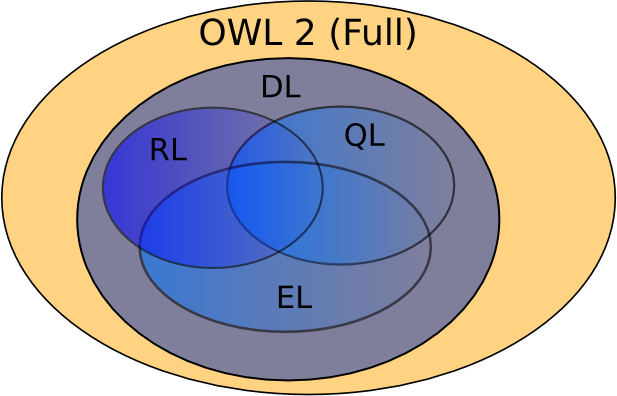
\includegraphics[clip,width=1\columnwidth,bb = 0 0 200 100, draft, type=eps]{/home/john/Desktop/Dissertation/figures/owl2-profiles.png}
\par\end{centering}
\caption{Componentes de um SAD \citet{junior2006sistemas}.\label{fig:Componentes-SAD}}
\end{figure}

A Figura \ref{fig:Componentes-SAD} mostra os componentes genéricos
de um SAD. Eles podem ser divididos em dados, banco de modelos, base
de conhecimento e interface de usuário; o banco de dados armazena
os dados não tratados, é importante que dito banco seja mantido atualizado
para um resultado confiável, o banco de modelos armazena vários modelos
que auxiliam a criação de cenários para a tomada de decisões, o banco
de conhecimento é produzido a partir do entendimento profundo do domínio
de conhecimento no qual são abstraídas as regras do sistema e a interface
de usuário representa cada camada do SADs para que o usuário interaja
com ele.

\section{Arquitetura para Sistemas de Apoio à Decisão}

A arquitetura de um software define a organização em termos de seus
componentes, suas interconexões, suas interações e também suas principais
propriedades \citet{de1997software}. Ela fornece as informações de
como os elementos envolvidos nela se relacionam. Arquiteturas trabalham
a parte externa das ligações entre seus elementos, implementações
internas desses elementos não são considerados arquiteturais \citet{sei2006architecture}.

SADs são criados por especialistas nas áreas de domínio nas quais
eles serão aplicados e implementados por programadores. Esse pode
ser um processo lento e custoso, já que os dois grupos de profissionais
têm \foreignlanguage{english}{\emph{backgrounds}} diferentes e vão
ter problemas de comunicação durante o processo de criação e testes
de um SAD. Esses profissionais podem ser até de organizações diferentes,
o que dificulta ainda mais o processo. Devido ao fato de que os elementos
básicos de todo o SAD (Figura \ref{fig:Componentes-SAD}) serem muito
parecidos, é possível criar uma arquitetura que possa ser re\nobreakdash-usada
em diferentes SADs (ou classes de SADs). Esta arquitetura pode ser
baseada em componentes de software re\nobreakdash-usáveis. Programadores
podem usar essa arquitetura e re\nobreakdash-usar os componentes
de software, já desenvolvidos para ela, para implementar SADs mais
rapidamente.

Para encontrar e configurar componentes de software de uma arquitetura,
uma opção é descrever esses componentes, usando uma ontologia, e usar
os termos dessa ontologia para encontrar os componentes corretos para
uma aplicação \citet{Linhalis2010}. Essas ontologias podem ser criadas
utilizando linguagens padrões da Web Semântica, como a Web Ontology
Language (OWL\nomenclature{OWL}{Web Ontology Language}), para melhor
portabilidade \citet{Pahl2007}. Ontologias e padrões da Web Semântica
serão abordados com mais profundidade no próximo capítulo.

Ontologias, que descrevam componentes de software para serem usados
num SAD de um determinado domínio, terão uma grande quantidade de
termos derivados desse domínio. Especialistas desse domínio terão
familiaridade com esses termos e poderão especificar grande parte
do fluxo de trabalho do SAD usando esses termos. Idealmente, essa
especificação deve ser detalhada o suficiente para que programadores
possam desenvolver a parte computacional do SAD sem necessidade de
mais feedback dos especialistas.

Como especialistas de domínio não têm um conhecimento muito detalhado
sobre linguagens de especificação de sistemas, é necessário o desenvolvimento
de uma \foreignlanguage{english}{Domain Specific Languag}e (DSL) adequada
ao nível de conhecimento de computação dos especialistas. Essa linguagem
também deve conter termos familiares ao domínio desses especialistas. 

\section{Considerações Finais}

Este capítulo apresentou os conceitos principais de SADs, incluindo
a definição geral e a arquitetura de software. Ele também apontou
para a necessidade da geração automática (ou semi\nobreakdash-automática)
de interfaces gráficas de usuários SADs. Uma abordagem para conseguir
a geração automática (ou semi\nobreakdash-automática) de GUIs consiste
na integração com DSLs, onde sejam definidas as características gerais
do sistema e integrado com os conceitos do domínio de conhecimento
a través das ontologias usadas nesses sistemas.


\chapter{Contexto: Ontologias e DSL\label{chap:Context}}

A partir do problema identificado e da revisão da literatura foi encontrado
que o desenvolvimento de ontologias é um área de pesquisa abrangida
pela Web Semântica que permite desenvolver sistemas web baseados em
conhecimento, satisfazendo os requisitos de desenvolvimento do SAD
SustenAgro explicados no capitulo \ref{chap:SAD}.

A web foi criada para possibilitar o acesso, intercâmbio e recuperação
de informações de maneira rápida e simples, seu crescimento exponencial
e caótico fez com que a mesma se tornasse hoje um gigantesco repositório
de documentos, o que dificulta a recuperação de informações. Até o
momento, não existe nenhuma estratégia abrangente e satisfatória para
a indexação de documentos por meio de “motores de busca” que seja
coerente com uma estrutura linguística. \citet{Souza:2004}.

Um exemplo da deficiência da web atual, pode ser identificada na busca
realizada pelos sistemas de recuperação de informação, que usam palavras-chave
nas buscas, onde apenas a similaridade e o número de ocorrências de
certas palavras no conteúdo de documentos são levados em consideração
e não a semântica presente naquela informação. \citep{Souza:2004}.

Neste capítulo, vamos apresentar e discutir os conceitos usados da
web semântica, exatamente: fundamentos da Web Semântica, Ontologias,
o \foreignlanguage{english}{Resource Description Framework (RDF)}
\nomenclature{RDF}{Resource Description Framework}, a \foreignlanguage{english}{Web
Ontology Language} (\foreignlanguage{english}{OWL})\nomenclature{OWL}{Web Ontology Language}
e finalmente as \foreignlanguage{english}{DSLs}\nomenclature{DSL}{Domain Specific Language}
que são linguagens de proposito especifico que permitem definir um
meio de comunicação entre os especialistas e o sistema desenvolvido.

\section{Web Semântica.}

A interpretação do significado é uma habilidade inata dos seres humanos,
através da associação dos conceitos que estão no cérebro por meio
de estruturas neurais, nas maquinas não existe esta habilidade, devido
a que um dado ou informação é um conjunto de caracteres sem associação
a conceitos, a Web Semântica procura determinar métodos para que as
maquinas aproximem-se nesta capacidade, atualmente é possível inferir
e deduzir informações, porem não deve confundir-se com a compreensão
humana.

A Web Semântica tem como finalidade estruturar os dados e informações
disponíveis na Web para que tenham significado e que seja computável,
gerando assim um ambiente onde agentes software e usuários possam
trabalhar de maneira cooperativa, está formada por um conjunto de
padrões propostos pelo \foreignlanguage{english}{World Wide Web Consortium}
(W3C) \nomenclature{W3C}{World Wide Web Consortium}, na figura \ref{fig:Semantic_Web_History}
podem ser observados os padrões que constituem a Web Semântica e sua
relação com os padrões \foreignlanguage{english}{XML} \nomenclature{XML}{Extensible Markup Language}. 

\begin{figure}[H]
\begin{centering}
\includegraphics[width=1\columnwidth]{\string"figures/Semantic Web History\string".png}
\par\end{centering}
\caption{História da Web Semântica \label{fig:Semantic_Web_History}}
\end{figure}

\citet{bernerslee2001} propuseram a Web Semântica no 2001, como uma
extensão da Web atual na que é possível vincular conceitos de maneira
estruturada e padronizada com a finalidade de gerar uma web universal
dos conhecimentos da humanidade; permitindo assim fornecer conhecimento
estruturado para que seja computável pelas maquinas, e gerar um meio
comum de representação entre os humanos e maquinas.

A partir desta visão conceitual sobre a Web, \citet{bernerslee2001}
propôs uma arquitetura que organiza as representações do conhecimento
por meio de camadas, dita arquitetura é conhecida como \foreignlanguage{english}{Semantic
Web Cake} que é ilustrada na Figura \ref{fig:Web-Semantic-Architecture}

\begin{figure}
\centering{}\includegraphics[width=0.8\columnwidth]{\string"figures/Semantic Web Architecture\string".png}\caption{Arquitetura em camadas da Web Semântica\label{fig:Web-Semantic-Architecture}}
\end{figure}

A base da arquitetura é estabelecida pelos padrões \foreignlanguage{english}{Unicode}
e URI, que padronizam a representação dos dados por meio das seguintes
camadas: 
\selectlanguage{english}%
\begin{description}
\item [{Unicode}] \foreignlanguage{brazil}{é um padrão que codifica os
caracteres na maioria dos sistemas de escrita para representação de
texto com fines de processamento computacional.}
\item [{URI}] \foreignlanguage{brazil}{\nomenclature{URI}{Uniform Resource Identifier}
permite identificar unificadamente os recursos disponíveis na Web
por meio de uma }String.
\item [{XML}] \foreignlanguage{brazil}{representa os dados de maneira sintática,
através a definição de }markups\foreignlanguage{brazil}{ os quais
codificam os documentos dando formato preestabelecido e permitindo
que as informações sejam legíveis tanto por humanos como por computadores,
suportando as camadas superiores na arquitetura da Web Semântica.}
\item [{RDF}] \foreignlanguage{brazil}{A camada de descrição que permite
especificar o domínio de conhecimento, também é usada como um método
geral para descrição conceitual o modelagem de informação por meio
de recursos, usa notações sintáticas e formatos de serialização.}
\item [{Ontology}] \foreignlanguage{brazil}{estende a camada de descrição,
fornecendo mais expressividade na definição de conceitos, relações
semânticas dos conceitos.}
\item [{Logic}] \foreignlanguage{brazil}{permite definir regras logicas
para deduzir e inferir novas informações que conseguem mudar a estrutura
da ontologia de maneira dinâmica.}
\item [{Proof}] \foreignlanguage{brazil}{fornece mecanismos para avaliar
o nível de confiabilidade das fontes de recursos e informações.}
\item [{Trust}] \foreignlanguage{brazil}{representa o conhecimento validado
e confiável.}
\item [{Digital-Signature}] \foreignlanguage{brazil}{permite integrar métodos
de segurança que garantam a confiabilidade da informação.}
\end{description}
\selectlanguage{brazil}%
Uma das contribuições da Web Semântica foi a formalização das ontologias,
as quais são definidas a continuação, no desenvolvimento desta pesquisa
incluiu-se desde as camadas inferiores até o \foreignlanguage{english}{OWL},
permitindo definir ontologias que representem os domínios de conhecimento.

\section{Ontologias}

\citet{Smith2007} descreve a ontologia como uma área da filosofia,
que estuda a natureza, existência e realidade dos entes, assim como
as categorias do ser e das relações semânticas.

Na ciências da computação e informação, a palavra ``ontologia''
define-se como uma especificação formal e explicita de uma conceitualização
compartilhada de um domínio de conhecimento.

\citet{allemang2011semantic} define as ontologias no contexto da
Web Semântica como um esquema de representação que permite conceitualizar
e estruturar conhecimento, permitindo a interpretação dele através
das computadoras, cujo principal objetivo é compartilhar conhecimento
entre humanos e computadoras.

Uma ontologia é um sistema de organização e representação do conhecimento,
em inglês\emph{ }\foreignlanguage{english}{\emph{Knowledge Organization
System}} (\foreignlanguage{english}{\emph{KOS}}), que é uma estrutura
conceitual e computacional que permite representar o conhecimento,
de qualquer domínio, por meio de entidades, classificações, relações
semânticas, regras e axiomas.

Uma ontologia é especificada por meio de componentes básicos que são
as classes, relações, axiomas e instâncias. As \textbf{classes}, o
foco da maioria das ontologias, são utilizadas para descrever os conceitos
de um domínio, possibilitando a organização e classificação dos indivíduos
em um sistema lógico e hierárquico contendo subclasses que representam
conceitos específicos \citet{noy2001ontology}. As \textbf{relações}
representam o tipo de interação entre os conceitos de um domínio e
as propriedades presentes nas classes e indivíduos. Elas podem ter
características próprias, como serem transitivas, simétricas, ou terem
uma cardinalidade definida. Os \textbf{axiomas} são utilizados para
modelar regras assumidas como verdadeiras no domínio em questão, de
modo que seja possível associar o relacionamento entre os indivíduos,
além de fornecer características descritivas e lógicas para os conceitos.
Por fim, os \textbf{indivíduos}, ou instâncias das classes, são utilizados
para representar elementos específicos, ou seja, os próprios dados,
que juntamente com a definição de uma ontologia, constituem a base
de conhecimento \citep{noy2001ontology}, os indivíduos representam
objetos do domínio de interesse \citet{horridge2011owl}.

Segundo \citet{Patel-schneider05buildingthe} a representação de ontologia
é realizada por meio de lógica de predicados e lógica descritiva,
usando padrões adotados pela comunidade como \foreignlanguage{english}{RDF}
e \foreignlanguage{english}{OWL}.

A Figura \ref{fig:Smart-data-continuum} mostra os níveis de representação
de dados na forma de conhecimento processável por máquinas.

\begin{figure}[H]
\centering{}\includegraphics[width=0.8\columnwidth]{\string"figures/smart data\string".png}\caption{\foreignlanguage{english}{Smart data continuum\foreignlanguage{brazil}{: níveis de representação
de dados na forma de conhecimento processável por máquinas.\label{fig:Smart-data-continuum}}}}
\end{figure}

O nível mais baixo de representação começa com os dados sem nenhum
significado semântico, dependentes do contexto da aplicação. O segundo
nível envolve a definição de esquemas \foreignlanguage{english}{XML}
para conseguir independência dos dados da aplicação, os dados fluem
entre aplicações em um único domínio mas não podem ser compartilhados
fora do domínio. No terceiro nível, os dados podem ser combinados
a partir de diferentes domínios, sendo suficientemente independentes
para serem recuperados e combinados com outras fontes de dados, finalmente
no quarto nível, é possível inferir novos dados a partir dos existentes
e compartilha-os entre aplicações sem requerer interferência humana
\citep{sugumaran2011}, cada uma destas caraterísticas compõem as
ontologias.
\selectlanguage{english}%

\section{Resource Description Framework\foreignlanguage{brazil}{ (}RDF\foreignlanguage{brazil}{)}}

\selectlanguage{brazil}%
O \foreignlanguage{english}{Resource Description Framework (RDF)}
é uma família de especificações da W3C, que foi disponibilizada em
1999 como parte do W3C's \foreignlanguage{english}{Semantic Web Effort},
que fornece um \foreignlanguage{english}{Framework} comum que permite
aos dados ser compartilhados e reusados através das fronteiras das
aplicações, empresas e comunidades \footnote{http://www.w3.org/2001/sw/}.
Ele foi originalmente projetado como um modelo de metadados e também
chegou a ser usado como um método de descrições conceituais, principalmente
para descrever recursos web. 

O \foreignlanguage{english}{RDF} é usado em várias áreas de aplicação,
como \foreignlanguage{english}{\emph{resource discovery}} para melhorar
as capacidades dos motores de busca, \foreignlanguage{english}{\emph{cataloging}}
para descrever o conteúdo e as relações de conteúdo disponibilizados
em um sistema web particular e descrição de \foreignlanguage{english}{\emph{intellectual
property rights}} de páginas web.

O modelo básico de dados consiste em um padrão de três tipos de objetos:
\begin{itemize}
\item Sujeito: representa os recursos e são identificados por meio de \foreignlanguage{english}{URIs},
sem importar o tamanho deles, por exemplo, uma pagina web ou um elemento
\nomenclature{HTML}{HyperText Markup Language} podem ser recursos.
\item Predicado: são aspectos, características, atributos ou relações especificas
que descrevem o sujeito, cada predicado têm um significado especifico
e relaciona um sujeito com um objeto.
\item Objeto: um recurso especifico ou valor da propriedade que representa
uma características do objeto \footnote{http://www.w3.org/TR/PR-rdf-syntax/}
\end{itemize}
Com \foreignlanguage{english}{RDF} é possível explicitar relações
entre dois objetos (usando-se uma Tripla \foreignlanguage{english}{RDF}),
mas não consegue fazer modelagens especificas nem integrar inferência.
Para descrever detalhadamente o que um objeto representa e suas relações
com outros objetos, são necessárias ontologias descritas no padrão
\foreignlanguage{english}{OWL} que será apresentado a continuação. 
\selectlanguage{english}%

\section{Web Ontology Language\foreignlanguage{brazil}{ (}OWL\foreignlanguage{brazil}{)}}

\selectlanguage{brazil}%
A \foreignlanguage{english}{Web Ontology Language} (\foreignlanguage{english}{OWL})
foi recomendada pelo W3C em 2004 para representar e compartilhar ontologias
na Web. Essa linguagem foi projetada para aplicações que necessitam
processar o conteúdo da informação em vez de apenas organizar informações
em nós \citet{mcguinness2004owl}. \foreignlanguage{english}{OWL}
é uma linguagem que permite que a semântica seja explicitamente associada
ao conteúdo dos dados na web e formalmente especificada através de
ontologias, compartilhadas na Internet. 

A versão \foreignlanguage{english}{OWL} 2 é a versão mais recente
da linguagem \foreignlanguage{english}{OWL}. De acordo com as especificações
do W3C\footnote{http://www.w3.org/TR/owl2-overview/}, a \foreignlanguage{english}{OWL
2} adicionou três novos perfis (\foreignlanguage{english}{sub-linguagens})
aos perfis DL e \foreignlanguage{english}{Full} já existentes: \foreignlanguage{english}{OWL
2} EL,\foreignlanguage{english}{ OWL 2 QL} e \foreignlanguage{english}{OWL
RL} (Figura \ref{fig:OWL2-Profiles}). Cada um desses perfis fornece
características de expressividade diferente para diversos cenários
de aplicação:

\begin{figure}[H]
\begin{centering}
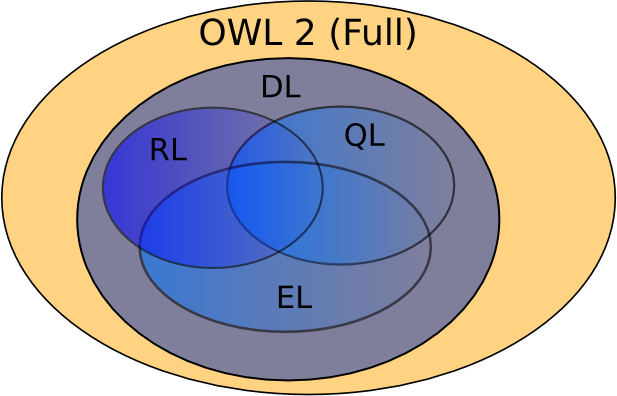
\includegraphics[width=0.8\columnwidth]{figures/owl2Profiles}
\par\end{centering}
\caption{OWL2 Profiles.\label{fig:OWL2-Profiles}}
\end{figure}

\selectlanguage{english}%
\begin{description}
\item [{Full}] \foreignlanguage{brazil}{O perfil }OWL Full\foreignlanguage{brazil}{
é direcionado para usuários que querem a máxima expressividade e a
liberdade sintática do }OWL\foreignlanguage{brazil}{ sem garantia
computacional. É improvável que qualquer motor de raciocínio seja
capaz de suportar completamente cada recurso da }OWL Full\foreignlanguage{brazil}{
\citep{mcguinness2004owl}.}
\selectlanguage{brazil}%
\item [{DL}] O perfil \foreignlanguage{english}{OWL DL} (\foreignlanguage{english}{Description
Logic}) é para aplicações que necessitam de máxima expressividade,
enquanto mantém a computabilidade (todas as conclusões são garantidos
para ser computáveis) e decidibilidade (todas as computações terminarão
em tempo finito) \citep{mcguinness2004owl}. \foreignlanguage{english}{OWL
DL} inclui as construções da linguagem \foreignlanguage{english}{OWL},
mas elas podem ser usadas somente sob certas restrições. 
\item [{EL}] O perfil \foreignlanguage{english}{OWL} 2 EL é baseado na
família EL++ de lógica descritiva (\foreignlanguage{english}{Description}
\foreignlanguage{english}{Logic}), esse perfil é particularmente útil
em aplicações utilizando ontologias que contêm um grande número de
propriedades e/ou classes. Além disso, o \foreignlanguage{english}{OWL}
2 EL utiliza um padrão comum utilizado em ontologias para conceitos
e planejamento, ou seja, a combinação de conjunção e qualidades existenciais.
\selectlanguage{english}%
\item [{QL}] \foreignlanguage{brazil}{O perfil }OWL 2 QL\foreignlanguage{brazil}{
é baseado na família }DL-Lite\foreignlanguage{brazil}{ de lógica descritiva,
esse perfil foi criado para permitir o raciocínio (}reasoning\foreignlanguage{brazil}{)
eficiente com grandes quantidades de dados estruturados de acordo
com esquemas relativamente simples, ele fornece a maioria dos recursos
necessários para capturar modelos conceituais, tais como diagramas
de classe UML, diagramas de entidade/relacionamento, e esquemas de
banco de dados. }
\selectlanguage{brazil}%
\item [{RL}] O perfil \foreignlanguage{english}{OWL 2 RL} é voltado para
aplicações que exigem raciocínio escalável em troca de alguma restrição
de poder expressivo. Ele define um subconjunto sintático de \foreignlanguage{english}{OWL
2} que favorece a implementação utilizando tecnologias baseadas em
regras, esse perfil pode ser utilizado na maioria das construções
\foreignlanguage{english}{OWL 2}, porém, para permitir implementações
baseadas em regras de raciocínio, a forma como essas construções podem
ser usadas em axiomas foi restringida. 
\end{description}
\selectlanguage{brazil}%
A ferramenta para definir ontologias da web semântica recomendada
pela comunidade e usada na presente pesquisa foi Protégé\footnote{Ferramenta e framework Protégé \url{http://protege.stanford.edu/}},
que permite um amplo suporte no processo de definição de ontologias.
\selectlanguage{english}%

\section{Domain Specific Language (DSL)\foreignlanguage{brazil}{ }}

\selectlanguage{brazil}%
Em desenvolvimento de software e engenharia de domínio uma linguagem
de domínio específico, em inglês \foreignlanguage{english}{\emph{Domain-Specific
Language}}\emph{ (DSL)}, é um tipo de linguagem de programação ou
linguagem de especificação, dedicada a um domínio particular de problema
com expressões propiás dos especialistas de aquele domínio.

Um usuário, relacionado com um domínio específico, pode usar uma DSL
sem ter experiência em desenvolvimento de software pois a DSL está
relacionada com seu domínio de trabalho, o autor \citet{fowler2010domain}
diz que programadores instruem o computador no que ele deve fazer,
pois já entendem a maneira dele trabalhar, mas com \foreignlanguage{english}{DSLs}
é feito o inverso: o computador começa a entender o que o programador
(usuário) escreve.

Segundo \citet{Mernik:2005:DDL:1118890.1118892} as vantagens das
DSL em comparação com as linguagens de proposito geral são a expressividade,
facilidade de uso e a integração com o domínio da aplicação. O conceito
não é novo, linguagens de programação de propósito especifico existiram
desde o começo das linguagens de programação, mas o termo tornou-se
padrão devido à ascensão da modelagem de domínio específico, elas
são classificadas em:
\selectlanguage{english}%
\begin{itemize}
\item Domain-Specific Markup Languages\foreignlanguage{brazil}{: são linguagens
de um domínio particular com a particularidade de anotar os dados
para que eles sejam sintaticamente distinguíveis, um exemplo deles
é o }Hypertext Markup Language ((HTML \nomenclature{HTML}{HyperText Markup Language})\foreignlanguage{brazil}{
que permite anotar dados no domínio das paginas web.}
\item Domain-specific modeling languages:\foreignlanguage{brazil}{ são linguagens
que permitem expressar informação, conhecimento o sistemas em uma
estrutura consistente com um conjunto de regras que permitem interpretar
o significado dos componentes modelados, um deste tipo de linguagens
é }Unified Modeling Language\foreignlanguage{brazil}{ (}UML\nomenclature{UML}{Unified Modeling Language }\foreignlanguage{brazil}{)
que permite especificar sistemas software.}
\item Domain-specific programming languages:\foreignlanguage{brazil}{ são
linguagens permitem a programação em alto nível aplicado a um domínio
especifico de conhecimento, um exemplo dele é a linguagem R que permite
a programação de conceitos estatísticos e geração de gráficos }
\end{itemize}
\selectlanguage{brazil}%
No caso do SAD SustenAgro, foi analisado que as ontologias permitem
uma definição detalhada do conhecimento do domínio, más o formato
das ontologias requer que os especialistas em sustentabilidade aprendam
os padrões da Web Semântica descrita neste capitulo, o qual não é
trivial, devido a que precisa um conhecimento profundo de modelagem
em formatos semânticos.

Pelo qual a definição de uma DSL particular para os especialistas
do domínio, permitiria fornecer uma solução compatível com os termos
específicos deles, com o qual seria possível a especialistas especificar
o SAD com um grau de detalhamento suficiente para definir o conhecimento
deles sem intervenção dos desenvolvedores de software, os especialistas
poderiam se tornar, na prática, programadores de seus próprios SADs.

A DSL fará uso e gerenciara a ontologia para organizar o conhecimento
do domínio em um formato compatível com as tecnologias web semântica
e assim definir o SAD SustenAgro, a DSL será uma interface entre o
especialista e a ontologia permitindo fornecer que os especialistas
definam ontologias da web semântica.

\begin{figure}
\begin{centering}
\includegraphics[width=0.8\columnwidth]{\string"figures/DSL Diagram\string".png}
\par\end{centering}
\caption{Camada da DSL \label{fig:Camada-da-DSL}}
\end{figure}


\section{Considerações finais}

Os conceitos apresentados anteriormente foram necessários para o desenvolvimento
da presente pesquisa, demostrando que a web semântica fornece o suporte
tecnológico e teórico suficiente para abordar o desenvolvimento de
sistemas baseados em conhecimento, particularmente as ontologias suportaram
vários aspectos cruciais no desenvolvimento deste projeto, pelo qual
elas foram o foco central da presente pesquisa. 

As DSL auxiliam a definição da ontologia, fornecendo uma linguagem
especifica para o especialista, conseguindo de esta maneira que os
especialistas definam o conhecimento deles no sistema SAD.


\chapter{Decisioner\label{chap:Decisioner}}

A partir da descrição das características do SAD SustenAgro (seção
\ref{sec:SAD-SustenAgro}), do requisito de modelar o conhecimento
através de ontologias (usando tecnologias da Web Semântica) e de definir
uma DSL para facilitar a definição de comportamentos por parte dos
especialistas, foi modelado e desenvolvido um protótipo de um framework,
intitulado Decisioner, que permite definir e gerar SADs do tipo do
SustenAgro. O framework Decisioner é basicamente formado por ontologias,
que representam conhecimento do domínio, e por uma DSL que permite
definir comportamentos e estabelecer configurações gerais de um SAD.

Satisfazer os requisitos requeridos pelos pesquisadores da Embrapa
Meio Ambiente foi uma das forças que dirigiram o desenvolvimento desta
pesquisa. Para chegar a arquitetura, aqui apresentada, houve um trabalho
interativo para chegar aos requisitos que eram gerais, que deveriam
estar no framework, e os que eram específicos, que deveriam estar
definidos na ontologia ou na DSL do SustenAgro. 

Neste capítulo será apresentado a arquitetura do protótipo Decisioner,
cada uns dos seus componentes e funcionalidades e as contribuições
para esta pesquisa.

\section{Arquitetura do Decisioner}

Os SADs, segundo a descrição feita no capítulo \ref{chap:SAD}, são
compostos por banco de dados, base de conhecimento, módulo de processamento
da informação e módulo gerador de resultados. Em cada um desses módulos,
está implícito o conhecimento dos especialistas, pelo qual a primeira
característica definida do Decisioner foi a integração de ontologias. 

As ontologias permitem a definição do conhecimento dos especialistas
em um componente independente. Ele é complementado pela DSL, que permite
definir comportamento e características do SAD. O diagrama para a
arquitetura desenvolvida para essa solução é apresentado na figura
\ref{fig:Componente-DSL}. Com base nesse diagrama, os componentes
dos SADs foram generalizados e, por meio do desenvolvimento de experimentos,
foi definida uma arquitetura que pode ser reusada em diferentes SADs
(do mesmo tipo do SustenAgro).

O Decisioner pode ser classificado como um framework. Já que é uma
plataforma de software com design reutilizável e implementações reutilizáveis
pelos clientes, que o especializam em um domínio particular \citep{RiehlePhdthesis}.

A arquitetura do framework Decisioner é composta pelos componentes
gerais para a definição de SADs, apresentados na Figura \ref{fig:Interfaces}.
Usuários especialistas podem interagir com o framework através dos
editores de ontologias e DSL. Usuários finais interagem através da
sua interface Web.

\begin{figure}[H]
\centering{}\includegraphics[width=0.9\columnwidth]{\string"figures/Decisioner Architecture\string".eps}\caption{Arquitetura do Decisioner\label{fig:Interfaces}}
\end{figure}

Os componentes dessa arquitetura são:
\selectlanguage{english}%
\begin{enumerate}
\item \textbf{Domain ontology}\foreignlanguage{brazil}{: representa os conceitos
específicos dos especialistas que serão utilizados no SAD.}
\item \textbf{Decisioner ontology}\foreignlanguage{brazil}{: faz uma ligação
entre os tipos de dados e as interfaces gráficas capazes de mostrar
ou editar esses dados, fazendo um mapeamento entre os dois.}
\item \textbf{Ontology Editor}\foreignlanguage{brazil}{: componente que
permite editar as ontologias em um formato mais fácil para o uso pelos
especialistas.}
\item \textbf{Triplestore}\foreignlanguage{brazil}{: sistema de armazenamento
e recuperação da informação em formato de triplas }RDF\foreignlanguage{brazil}{,
(explicado em detalhe na seção \ref{subsec:Triplestore}). Ele permite
o gerenciamento de dados e ontologias em formato }RDF.\foreignlanguage{brazil}{
A traves da linguagem padrão }SPARQL Protocol and RDF Query Language
(Sparql)\foreignlanguage{brazil}{ \citep{prud2006sparql}. }
\item \textbf{DSL code}\foreignlanguage{brazil}{: representa uma instancia
da DSL com as definições particulares para um SAD específico.}
\selectlanguage{brazil}%
\item \textbf{DSL Editor}: Editor visual web da DSL com recursos como \foreignlanguage{english}{code
completion} e \foreignlanguage{english}{syntax coloring}. Permite
a edição da \foreignlanguage{english}{DSL} por parte dos especialistas
do domínio.
\selectlanguage{english}%
\item \textbf{Web components}:\foreignlanguage{brazil}{ conjunto de elementos
visuais que podem ser reusados nos SADs com a finalidade de modularizar
e simplificar a geração de }Web User Interfaces\foreignlanguage{brazil}{
(UI\nomenclature{UI}{User Interface}).}
\item \textbf{DSL Interpreter}\foreignlanguage{brazil}{: Interpretador
da DSL para processar as definições do SAD e criar um SAD específico.
Ele usa a DSL, ontologias e componentes web para gerar automaticamente
a interface e comportamento de um SAD específico.}
\item \textbf{Web UI}\foreignlanguage{brazil}{: Interfaces visuais geradas
pelo }DSL Interpreter.\foreignlanguage{brazil}{ Utilizam os }Web Components\foreignlanguage{brazil}{
e fornecer a interface gráfica, usadas pelos usuários finais, na interação
com o SAD na Web.}
\end{enumerate}
\selectlanguage{brazil}%
Essa arquitetura foi implementada em um protótipo Decisioner. Sempre
que possível, na implementação do Decisioner, foram reutilizados componentes
ou bibliotecas disponíveis publicamente na internet.

\section{Metodologia}

Com a finalidade de desenvolver o protótipo do framework Decisioner,
escolheu-se o SAD SustenAgro como um caso de uso e exemplo de instanciação.
Ele permitiu a definição de uma metodologia de desenvolvimento para
os componentes. Teria sido interessante instanciar o framework para
um segundo SAD, para demonstrar melhor sua generalidade. Contudo,
dada as limitações de tempo impostas a um trabalho de mestrado e ao
tempo necessário ao desenvolvimento do framework, isso não foi possível.
No decorrer deste texto, foram feitas algumas considerações sobre
a generalidade do framework. A metodologia abordada durante este processo,
incluiu as seguintes etapas:
\begin{enumerate}
\item Seleção da \foreignlanguage{english}{Triplestore}: foram avaliadas
as \foreignlanguage{english}{triplestores} existentes com a finalidade
de definir uma que se adaptasse aos requisitos do framework.
\item Seleção da linguagem de programação e framework web: foi realizada
uma verificação das tecnologias de desenvolvimento de sistemas web
compatíveis com as tecnologias da web semântica e com a \foreignlanguage{english}{DSL}.
\item Design da DSL: Durante o processo de desenvolvimento do SAD SustenAgro,
foram generalizados seus componentes, permitindo definir cada uma
das características da DSL. O processo foi iterativo, permitindo refinar
a expressividade da linguagem com a ajuda de especialistas da Embrapa.
\item Desenvolvimento do \foreignlanguage{english}{DSL editor}: implementação
de uma \foreignlanguage{english}{web UI} que permite editar a DSL
em formato textual, fornecendo aos especialistas um editor moderno.
Modificações na DSL podem ser vistas no SAD imediatamente.
\item Desenvolvimento do \foreignlanguage{english}{Ontology Editor}: implementação
de uma \foreignlanguage{english}{web UI} com componentes específicos
para suportar a edição das ontologias, por parte dos especialistas,
em um formato textual.
\item Desenvolvimento do \foreignlanguage{english}{DSL Interpreter}: o interprete
da Decisioner DSL. Esse componente tinha que ser atualizado a medida
que o design da DSL mudava.
\item Integração com \foreignlanguage{english}{web components} e \foreignlanguage{english}{web
UI}s: \foreignlanguage{english}{Widgets} gráficas, na forma de \foreignlanguage{english}{Web
components} suportam a geração das \foreignlanguage{english}{Web UIs}
que compõem os SADs. \foreignlanguage{english}{Widgets} foram adicionadas
para atender as necessidades do SustenAgro.
\end{enumerate}
A metodologia de desenvolvimento foi guiada pelo desenvolvimento do
SAD SustenAgro. Primeiramente foram desenvolvidas as ontologias, continuando
com o desenvolvimento do \foreignlanguage{english}{DSL Interpreter}
e depois com a integração dos \foreignlanguage{english}{web components}
e \foreignlanguage{english}{UI}s. Foram realizados vários ciclos de
desenvolvimento para refinar as funcionalidades. A Figura \ref{fig:Metodologia-do-Decisioner}
representa a metodologia realizada.

\begin{figure}
\begin{centering}
\includegraphics[width=0.9\columnwidth]{\string"figures/Decisioner Methodology\string".eps}
\par\end{centering}
\caption{Metodologia de desenvolvimento do Decisioner\label{fig:Metodologia-do-Decisioner}}

\end{figure}

A seguir, cada componente da arquitetura do Decisioner é discutido,
começando pela ontologia Decisioner.

\section{Ontologia Decisioner\label{sec:Ontologia-Decisioner}}

Para desenvolver um protótipo de uma ontologia geral, que abstraísse
os conceitos dos SADs, foram analisados os sistemas SAD desenvolvidos
pela Embrapa Meio Ambiente, descritos na seção \ref{sec:SAD-SustenAgro}.

A versão inicial da ontologia foi modelada na ferramenta Protégé,
no formato \foreignlanguage{english}{OWL}. Depois foi criado um novo
formato, usando o \foreignlanguage{english}{YAML Ain't Markup Language
(YAML \nomenclature{YAML}{YAML Ain't Markup Language\\})}, mais simples
que \foreignlanguage{english}{OWL}, para ser usado pelos especialistas
no \foreignlanguage{english}{Ontology Editor}, explicado na seção
\ref{sec:Ontology-Editor}.

A ontologia Decisioner contém os elementos comuns identificados e
abstraídos dos SADs da Embrapa, e tem o proposito de fornecer uma
ontologia geral que dê suporte a SADs diferentes. 

\begin{figure}[H]
\centering{}\includegraphics[scale=0.7]{\string"figures/DSS ontology\string".eps}\caption{Modelagem abstrata do SAD\label{fig:Modelagem-do-SAD}}
\end{figure}

Na Figura \ref{fig:Modelagem-do-SAD}, é apresentada a hierarquia
de classes resultante. Ela contém as classes:
\selectlanguage{english}%
\begin{description}
\item [{Evaluation\ Object\foreignlanguage{brazil}{:}}] \foreignlanguage{brazil}{classe
que representa os objetos que serão analisados em cada processo de
avaliação. Eles serão indivíduos dessa classe ou de alguma subclasse
dela.}
\item [{Feature\foreignlanguage{brazil}{:}}] \foreignlanguage{brazil}{classe
que representa as caraterísticas a avaliar em um }Evaluation Object.\foreignlanguage{brazil}{
Elas serão quantificadas, analisadas e usadas no processo de geração
de relatórios no processo de avaliação. As }Features\foreignlanguage{brazil}{
têm associado um }Value\foreignlanguage{brazil}{ que as quantifica.
Existe a subclasse }\textit{Weighted}\foreignlanguage{brazil}{ que
representa uma }Feature\foreignlanguage{brazil}{ vinculada a um peso.
Esse peso pode ser usado nas fórmulas para o cálculo dos modelos codificados
pelos especialistas.}
\item [{Place\foreignlanguage{brazil}{:}}] \foreignlanguage{brazil}{classe
que representa a localização física dos objetos modelados, permitindo
referenciar geograficamente um }Evaluation Object.
\item [{Analysis\foreignlanguage{brazil}{:}}] \foreignlanguage{brazil}{classe
que representa uma avaliação associada a um }Evaluation Object\foreignlanguage{brazil}{.
Suas instâncias têm propriedades, como nome e data da avaliação, e
correspondem a uma avaliação cadastrada.}
\item [{Value\foreignlanguage{brazil}{:}}] \foreignlanguage{brazil}{classe
que representa os valores que são atribuídos a cada instância de }Feature.\foreignlanguage{brazil}{
As subclasses }Real\foreignlanguage{brazil}{ e }Categorical\foreignlanguage{brazil}{
representam tipos de valores.}
\item [{User\foreignlanguage{brazil}{:}}] \foreignlanguage{brazil}{classe
que representa os usuários do sistema.}
\item [{Role\foreignlanguage{brazil}{:}}] \foreignlanguage{brazil}{classe
que representa os papéis de usuário do sistema e suas permissões.
Por padrão, estão instanciados os perfis }User\foreignlanguage{brazil}{
e }Admin.
\end{description}
\selectlanguage{brazil}%
A partir dessas classes é possível organizar os conceitos específicos
de cada SAD como subclasses delas. Um aspecto importante das ontologias
é que suportam a inferência de novos conhecimentos, permitindo classificar
e relacionar dados novos do sistema, ajudando desta maneira na automatização
da geração dos SADs. Isso permite ao \foreignlanguage{english}{DSL
Interpreter} mapear qualquer conceito novo, específico de um SAD em
particular, a um desses conceitos conhecidos e saber o que deve ser
feito com ele. 
\selectlanguage{english}%

\section{Ontology Editor\label{sec:Ontology-Editor}}

\selectlanguage{brazil}%
Para suportar a edição das ontologias do domínio, por parte dos especialistas,
foi implementado um editor web. Ele permite editar a ontologia específica
do SAD em um formato baseado em \foreignlanguage{english}{YAML,} a
descrição da ontologia neste formato passa a um conversor para ficar
no formato \foreignlanguage{english}{OWL} que é processado pela \foreignlanguage{english}{API}
de protégé para instanciar a ontologia com as restrições definidas
e finalmente exportado como \foreignlanguage{english}{RDF} para ser
substituído na \foreignlanguage{english}{triplestore} \foreignlanguage{english}{Blazegraph,}
este processo é realizado a cada vez que o usuário salva a ontologia.

A Figura \ref{fig:Editor-de-ontologia} mostra uma imagem do editor.
Ela mostra o código da ontologia em formato \foreignlanguage{english}{YAML},
um \foreignlanguage{english}{side panel,} que apresenta as classes,
propriedades e indivíduos hierarquicamente (permitindo a referenciação
dos elementos no código), um \foreignlanguage{english}{button restore}
para restituir a ultima versão da ontologia e um \foreignlanguage{english}{button
save} para salvar e carregar no Decisioner a ontologia em edição.

Idealmente, especialistas de domínio deveriam poder criar a ontologia
usando um editor gráfico. Mas devido as restrições de escopo de um
projeto de mestrado, não haveria tempo para criar um. A criação de
uma ferramenta, como um editor gráfico, teria o escopo de um novo
mestrado. 

Usar um editor para \foreignlanguage{english}{OWL}, como o Protégé,
exigiria que os especialistas de domínio aprendessem \foreignlanguage{english}{OWL}
e lógica descritiva, o que não é uma opção viável. Este editor de
ontologias é uma solução intermediária. Ele adota um formato em \foreignlanguage{english}{YAML},
menos complexo que \foreignlanguage{english}{OWL}, mas expressivo
o suficiente para as necessidades das ontologias. Ele ajuda os usuários
a encontrar os elementos da ontologia (\foreignlanguage{english}{side
panel}) e permite a inserção da ontologia no Decisioner. Apesar de
ser possível aos especialistas desenvolver uma ontologia totalmente
nova, usando o editor, seu objetivo é permitir que eles possam fazer
modificações localizadas nas ontologias. 
\begin{flushleft}
\begin{figure}[H]
\begin{centering}
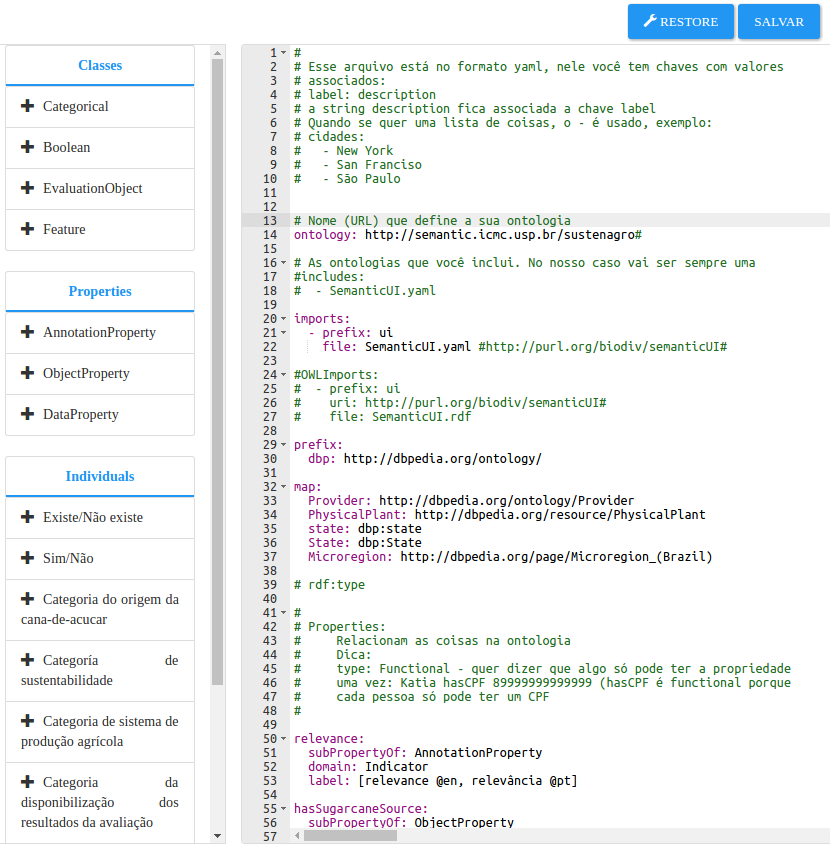
\includegraphics[width=1\columnwidth]{figures/SustenAgro-ontology-editor}
\par\end{centering}
\caption{Editor de ontologia\label{fig:Editor-de-ontologia} }
\end{figure}
\par\end{flushleft}

A ontologia definida em este editor será usada para definir a estrutura
dos SADs, as funcionalidades dos SADs são descritas na DSL apresentada
a continuação. 

\section{Decisioner DSL}

Para permitir que os especialistas definam o comportamento do framework
Decisioner, foi definida uma DSL que permite definir as principais
características de um SAD. Tal DSL foi baseada na modelagem geral
da arquitetura do \foreignlanguage{english}{Decisioner} e permite
relacionar conceitos específicos dos especialistas, criar equações
para os modelos usados, gerar a interface web para o usuário final,
servindo de interface entre a ontologia do Decisioner e a ontologia
do domínio.

A DSL foi baseada na linguagem \foreignlanguage{english}{Groovy},
porque ela suporta o desenvolvimento de \foreignlanguage{english}{DSLs}
que se comportam como extensões da linguagem \foreignlanguage{english}{Groovy}.

O uso da DSL, por parte especialistas, diminui o esforço necessário
no desenvolvimento de um SAD. Ela permite que os próprios especialistas
sejam capazes de fazer parte do desenvolvimento e validação do SAD.
Especialmente na parte de refinamento e atualização do SAD, especialistas
podem fazer modificações no sistema sem a ajuda de programadores e
ver o resultado dessas mudanças imediatamente.

As instruções definidas na DSL são:
\selectlanguage{english}%

\subsection*{Evaluation Object}

\selectlanguage{brazil}%
Nos SAD focados na avaliação, existe um objeto de avaliação que representa
as entidades a serem avaliadas. Esse objeto é constituído por propriedades
que especificam o que está sendo avaliado. A instrução \foreignlanguage{english}{\textit{evaluationObject}}\textit{
}permite definir as propriedades desse objeto. Por exemplo, caso uma
fazenda esteja sendo avaliada, é possível criar propriedades como
nome, tipo de produção, localização, etc.

A instrução tem como argumentos a URI (ou label) da classe da ontologia
do domínio, que será objeto de avaliação, e cada uma das propriedades
relacionadas. O algoritmo \ref{alg:Defini=0000E7=0000E3o-do-Evaluation}
apresenta um exemplo que usa a classe \textit{ProductionUnit}, como
classe dos objetos a serem avaliados e define as propriedades \textit{hasName},
para nome, e \textit{hasAgriculturalProductionSystem}, para tipo de
produção. Podem ser usados os labels das propriedades, ao invés de
suas URIs\textit{.}

\begin{algorithm}[H]
\inputencoding{latin9}\begin{lstlisting}
evaluationObject ":ProductionUnit", {     
 instance "ui:hasName', label: ["en": "Name", "pt": "Nome"]
 instance ":hasAgriculturalProductionSystem"
 type label: ["en": "Type", "pt": "Tipo"]
}
\end{lstlisting}
\inputencoding{utf8}
\caption{Definição do Evaluation Object\label{alg:Defini=0000E7=0000E3o-do-Evaluation}}
\end{algorithm}

O comando \foreignlanguage{english}{\textit{instance}} vincula uma
propriedade definida na ontologia, através da URI. Ela pode ser complementada
por parâmetros que customizam a representação visual da propriedade.
O comando \foreignlanguage{english}{\textit{type}} faz com que os
\foreignlanguage{english}{EvaluationObject} tenham que ser de subclasses
da classe principal. Por exemplo, uma unidade produtiva pode ser uma
plantação greenfield (mecanizada e uniforme), fazenda familiar, etc.
Os parâmetros que podem complementar as instruções anteriores são:
\selectlanguage{english}%
\begin{enumerate}
\item \textit{required}\foreignlanguage{brazil}{: define uma propriedade
obrigatória}
\item \textit{label}\foreignlanguage{brazil}{: define um texto associado}
\item \textit{placeholder}\foreignlanguage{brazil}{\textit{:} define um
texto de ajuda}
\item \textit{widget}\foreignlanguage{brazil}{: define um controle gráfico
de usuário}
\end{enumerate}

\subsection*{Feature}

\selectlanguage{brazil}%
A instrução \foreignlanguage{english}{\textit{Feature}} define as
características, do Evaluation Object, que serão usadas na sua avaliação.
O DSL Interpreter vai gerar uma interface gráfica, onde o usuário
final terá que preencher os dados sobre cada característica. Cada
característica tem um tipo associado a ela (na ontologia de domínio).
A partir dele, é possível associar uma widget específica para edição.
Por exemplo, a Figura \ref{fig:Widgets-geradas-da-DSL} mostra a
widget para uma característica que tem um tipo categórico com 3 possíveis
valores. Os textos mostrados vêm da ontologia e fazem parte da descrição
de cada elemento. É possível criar descrições em mais de uma língua.

\begin{figure}[H]
\begin{centering}
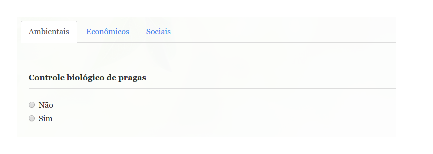
\includegraphics[width=0.8\columnwidth]{figures/IndicatorSelection}
\par\end{centering}
\caption{Widget geradas a partir da definição da DSL\label{fig:Widgets-geradas-da-DSL}}
\end{figure}

Quando o usuário final usa a widget, o valor escolhido é anotado,
no Evaluation Object, usando a propriedade \foreignlanguage{english}{\textit{has
value}}. Nas fórmulas, usadas para os cálculos do modelo usado, é
possível acessar esses valores. Os usuários não precisam preencher
a todas as características.

\begin{algorithm}[H]
\inputencoding{latin9}\begin{lstlisting}
feature ':EnvironmentalIndicator', 'extraFeatures': true
\end{lstlisting}
\inputencoding{utf8}
\caption{Definição de Features\label{alg:Defini=0000E7=0000E3o-de-Features}}
\end{algorithm}

O comando tem como argumento uma URI (ou label) (Algoritmo \ref{alg:Defini=0000E7=0000E3o-de-Features})
que vincula todas as subclasses da classe referenciada. O parâmetro
opcional \foreignlanguage{english}{\textit{extraFeatures}} permite
ativar a inserção de novas\foreignlanguage{english}{\textit{ features}},
por parte do usuário do SAD. 
\selectlanguage{english}%

\subsection*{Report}

\selectlanguage{brazil}%
O comando \foreignlanguage{english}{\textit{Report}} permite definir
as fórmulas e procedimentos matemáticas necessários para o cálculo
do modelo usado pelos especialistas de domínio, e como os resultados
serão apresentados (Algoritmo \ref{alg:Defini=0000E7=0000E3o-da-l=0000F3gica}).
Fórmulas e procedimentos para modelagem matemática são de responsabilidade
dos especialistas de domínio. A DSL permite desde fórmulas simples,
de uma linha, até o uso de bibliotecas complexas, chamadas usando
a JVM. Como a DSL é uma extensão da linguagem Groovy, qualquer comando
da linguagem pode ser usado nela, incluindo operações lógicas e aritméticas.
Para facilitar o trabalho dos especialistas de domínio, recomenda-se
encapsular qualquer algoritmo ou chamada de função mais complicados
num comando simples.

As fórmulas usadas têm acesso a todos os dados associados às \foreignlanguage{english}{\textit{Features}},
pelos usuários finais. Esses dados são usados no modelo adotado e
podem gerar múltiplos resultados de avaliação. No algoritmo \ref{alg:Defini=0000E7=0000E3o-da-l=0000F3gica},
o comando \textit{weightedSum(data.':EnvironmentalIndicator')} calcula
a média ponderada de todos os indicadores ambientais fornecidos pelo
usuário final. Esse comando foi criado para simplificar o trabalho
dos especialistas. Biblioteca de comandos, como essa, podem ser adicionadas
ao framework ou criados a pedido dos especialistas.

\begin{algorithm}[H]
\inputencoding{latin9}\begin{lstlisting}
report {     
 environment = weightedSum(data.':EnvironmentalIndicator')
 economic = weightedSum(data.':EconomicIndicator')
 social = weightedSum(data.':SocialIndicator')
 sustainability = (environment + social + economic)/3
 ...
}
\end{lstlisting}
\inputencoding{utf8}
\caption{Definição da lógica de avaliação.\label{alg:Defini=0000E7=0000E3o-da-l=0000F3gica}}
\end{algorithm}

Os resultados do processo de avaliação podem ser apresentados por
meio de várias \foreignlanguage{english}{\textit{widgets}} que facilitam
a representação e compreensão dos resultados da avaliação. No algoritmo
\ref{alg:Defini=0000E7=0000E3o-dos-componentes} o comando \textit{sustainabilityMatrix
x: sustainability, y: efficiency} apresenta os valores das variáveis
\textit{sustainability} e \textit{efficiency} num gráfico de matriz
de sustentabilidade (Figura \ref{fig:Matriz-de-sustentabilidade-widget}).
Para executar esse comando, o DSL Interpreter simplesmente coloca
a widget \textit{suatainabilityMatrix} na UI e passa os valores das
variáveis, como atributos. A widget vai ser responsável por criar
o gráfico. Essas widgets gráficas podem ser criadas como Web Components
 padrão (HTML 5) ou componentes do framework Grails (Seção \ref{sec:Web-components}
). O framework vem com um conjunto de widgets predefinidos, mas novas
podem ser adicionadas. 

\begin{algorithm}[H]
\inputencoding{latin9}\begin{lstlisting}
report {
 ...
 sustainabilityMatrix x: sustainability, y: efficiency
 text 'en': 'Microregion map', 'pt': 'Mapa da microregi�o'
 map data.'Microregion'
}
\end{lstlisting}
\inputencoding{utf8}
\caption{Definição dos componentes visuais do relatório.\label{alg:Defini=0000E7=0000E3o-dos-componentes}}

\end{algorithm}

Por meio dos comandos da DSL, é possível definir o comportamento e
as características gerais dos SAD. 

Os elementos gráficos (widgets), seja os que representam as Features
ou os usados nos relatórios, são implementados como \foreignlanguage{english}{Web
Components} HTML 5 ou Grails. Isso dá muita flexibilidade ao framework
Decisioner. A qualquer tempo é possível se acrescentar novas widgets,
para novos tipos de dados (Features) ou gráficos de relatórios. 
\selectlanguage{english}%

\section{DSL Editor}

\selectlanguage{brazil}%
Para suportar a edição da Decisioner DSL, foi implementado um editor
textual web que permite aos especialistas editar e rodar o código
da DSL. Ele é composto por um editor de código para a DSL, um \foreignlanguage{english}{button
restore} para carregar novamente a última versão válida da DSL e um
\foreignlanguage{english}{button save} para salvar e carregar a DSL
no DSL Interpreter. 

O Editor de código foi baseado no \foreignlanguage{english}{Ace Editor}\footnote{\url{ttps://ace.c9.io/}},
que fornece \foreignlanguage{english}{Syntax highlighting} para varias
linguagens de programação, entre elas Groovy, e como a DSL foi baseada
em Groovy, foi configurada para reconhecer dita sintaxe, também foi
ativado o suporte de \foreignlanguage{english}{code completion} para
fornecer uma experiência de uso amigável. A principal vantagem é a
funcionalidade de salvar a ontologia e reconfigurar o SAD imediatamente,
permitindo uma experiência em tempo real de redefinição do SAD, se
o usuário errar, ele vai poder restaurar as configurações por \foreignlanguage{english}{default}.

A Figura \ref{fig:Editor-DSL} mostra o editor em ação.

\begin{figure}[H]
\begin{centering}
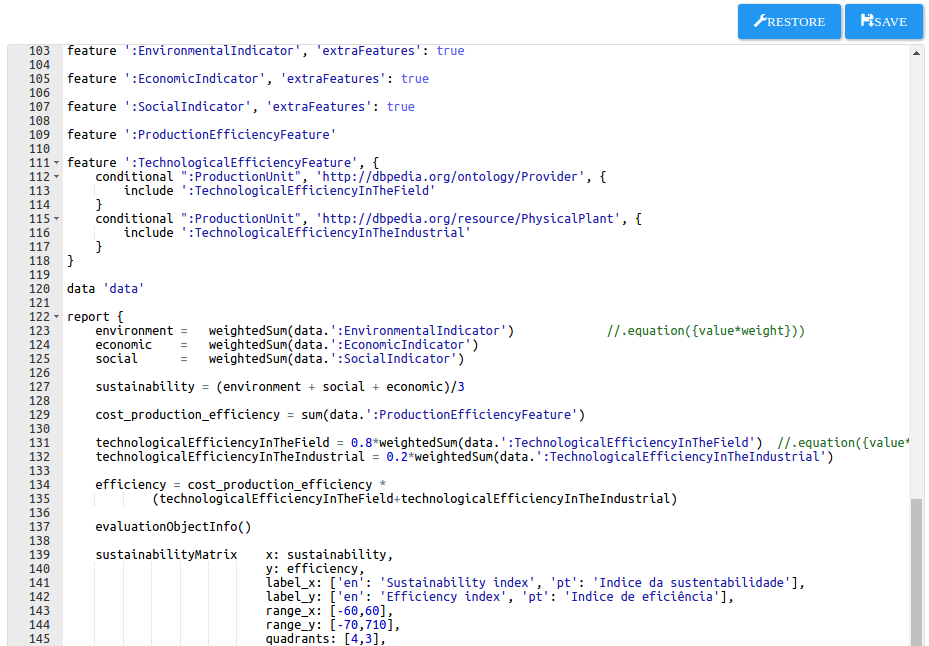
\includegraphics[width=1\columnwidth]{figures/SustenAgro-dsl-editor-2}
\par\end{centering}
\caption{Editor DSL\label{fig:Editor-DSL}}
\end{figure}

O editor da DSL tem compatibilidade com \foreignlanguage{english}{web
components}, tanto os fornecidos pelas bibliotecas integradas no Framework
Decisioner, como com os \foreignlanguage{english}{web components}
do Framework \foreignlanguage{english}{Grails} e adicionalmente podem
ser definidos \foreignlanguage{english}{web components }especializados.
\selectlanguage{english}%

\section{Web components\label{sec:Web-components}}

Web Component\foreignlanguage{brazil}{s }\footnote{\selectlanguage{brazil}%
Site oficial de \foreignlanguage{english}{web components} \url{https://www.webcomponents.org/introduction}\selectlanguage{brazil}%
}\foreignlanguage{brazil}{ é um conjunto de APIs padrão para definir
novas tags }HTML\foreignlanguage{brazil}{ personalizadas, reutilizáveis
e encapsuladas para o uso em páginas ou aplicações web. O framework
Grails também disponibiliza o uso de layout templates para implementar
partes reusáveis de uma view (página HTML). Com essas duas tecnologias,
é possível a criação de componentes (ou widgets) reusáveis da UI. }

\selectlanguage{brazil}%
Para suportar a geração de diferentes tipos de SADs, foi necessário
disponibilizar vários tipos de widgets que permitissem visualizar
e editar diferentes tipos de dados. Para relacionar os \foreignlanguage{english}{web
components} com o conhecimento dos especialistas, modelou-se, na ontologia
Decisioner, os \foreignlanguage{english}{data-types} que permitem
relacionar os tipos de dados com widgets específicas (capazes de edita-los),
usadas nas \foreignlanguage{english}{web UIs} dos SADs gerados. Os
dados das Features dos SADs podem ser de vários tipos e, para cada
tipo, existe uma widget apropriada para visualiza-o. Por exemplo,
para representar uma propriedade de tipo numérico discreto é possível
usar uma widget visual tipo \foreignlanguage{english}{spinner}.

Nos relatórios, os especialistas devem contar com widgets para apresentar
seus resultados em vários formatos, como tabelas, mapas, matriz de
sustentabilidade, etc. Essas widgets podem ser específicas para um
tipo de SAD em particular. Por isso, além do framework contar com
uma biblioteca de widgets prontas, deve ser possível adicionar novas
widgets facilmente. Ao usar padrões, como para Web Components, o framework
permite a fácil inclusão de widgets novas. Não se espera que os especialistas
de domínio criem essas widgets, mas sim que seja fácil para eles consegui-las
de desenvolvedores independentes (que só precisam conhecer o padrão
para Web Components e os requisitos da widget). 

O framework Decisioner tem uma biblioteca de \foreignlanguage{english}{web
components} (widget) construída usando o\foreignlanguage{english}{
web framework Bootstrap }\footnote{\url{http://getbootstrap.com/}},
que conta com diversos componentes básicos para a geração das Web
UI. A maioria deles foi definida usando as \foreignlanguage{english}{layout
templates} do framework \foreignlanguage{english}{Grails}, por ser
mais fácil de programar. Atualmente, apenas dois componentes usam
Web Components.
\selectlanguage{english}%

\section{Web UI}

\selectlanguage{brazil}%
A \foreignlanguage{english}{Web UI} é uma interface web de usuário
responsável por toda a interação com o usuário final. Ela permite
apresentar e editar as informações do SAD, gerar as análises e visualizar
os resultados na web ou em relatórios impressos. O mais importante
é que ela é gerada automaticamente pelo DSL Interpreter, usando a
DSL e ontologias particulares a cada SAD. 

Parte da Web UI é igual para todos os SADs, como formulários de login.
O resto dela é gerado com a ajuda dos \foreignlanguage{english}{Web
Components.} Eles são relacionadas aos tipos de dados existentes no
sistema, por meio da ontologia Decisioner. Por exemplo, dados podem
ser dos tipos numérico contínuo, numérico discreto, percentagem, booleano,
categóricos ou alfanumérico. Dada essa diversidade, os tipos de dados
foram modelados em ontologias com a finalidade de permitir a adaptação
automática (ou semiautomática) da interface às mudanças dos conceitos
do domínio.

Mudanças no layout geral podem ser feitas também através da edição
das \foreignlanguage{english}{Cascading Style Sheets (CSS \nomenclature{CSS}{Cascading Style Sheets})}
do Decisioner. É esperado que, quando da instalação do sistema, técnicos
de informática façam uma customização do sistema para adequá-lo aos
padrões de apresentação da instituição. Eles também devem incluir
qualquer Web Component (widget) necessário mas não disponível por
default no Decisioner. 

A figura \ref{fig:Web-UI} apresenta uma Web UI que foi gerada automaticamente,
a partir da ontologia e das definições na DSL do SAD SustenAgro. Nela
são apresentados vários tipos de \foreignlanguage{english}{Web Components}
que demostram o suporte a diferentes tipos de dados.

\begin{figure}[H]
\begin{centering}
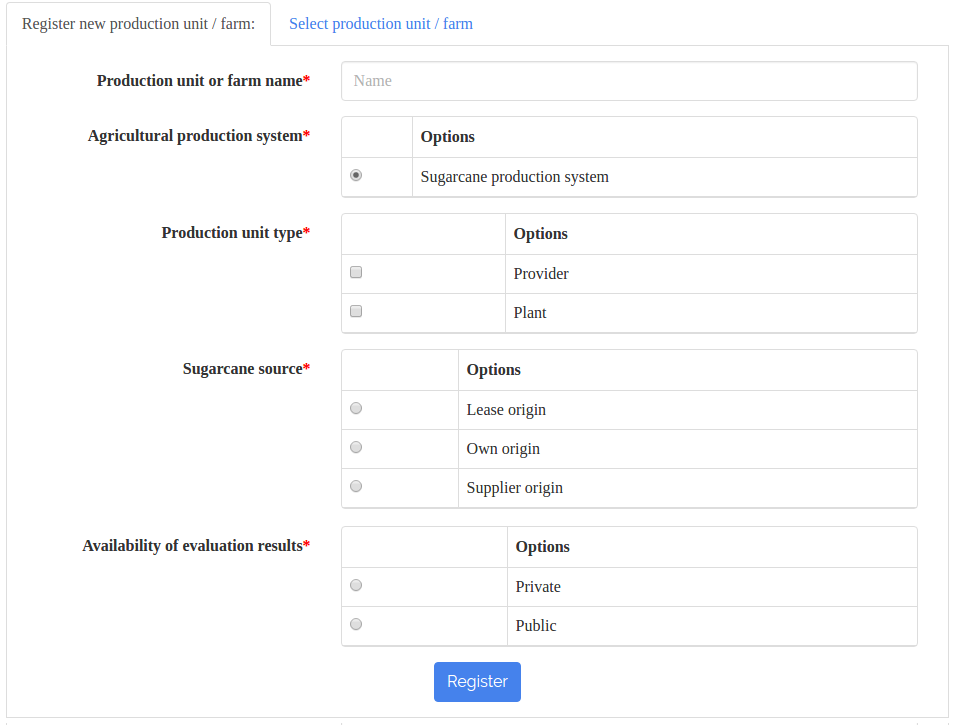
\includegraphics[width=1\columnwidth]{figures/SustenAgro-tool}
\par\end{centering}
\caption{\foreignlanguage{english}{Web UI \foreignlanguage{brazil}{com} web components\label{fig:Web-UI}}}
\end{figure}

\selectlanguage{english}%

\section{DSL Interpreter}

\selectlanguage{brazil}%
O DSL Interpreter é o principal modulo do framework Decisioner. A
sua principal funcionalidade é a interpretação das \foreignlanguage{english}{DSLs}.
Ele executa cada uma das instruções da DSL, vinculando dados e informação,
das ontologias ou fornecidos pelos usuários finais, aos \foreignlanguage{english}{web
components} com a finalidade de gerar as Web \foreignlanguage{english}{UIs}.

Para interagir com os dados da ontologia e apresenta-los na linguagem
dos especialistas, foi necessário criar, no DSL Interpreter, uma camada
de consulta de dados na \foreignlanguage{english}{triplestore} para
simplificar as consultas SPARQL (Figura \ref{fig:Arquitetura-do-Decisioner-Core}).
Esta camada, Sparql Simplifier, foi desenvolvida como uma solução
eficiente para a recuperação de informações semânticas de um domínio
de conhecimento usando um formato simplificado. 

O componente \foreignlanguage{english}{DSL Interpreter} processa
as instruções dos especialistas na linguagem Decisioner DSL. Foram
utilizadas técnicas padrões para a criação de DSLs usando a linguagem
\foreignlanguage{english}{Groovy\citep{dearle2015groovy},} o que
facilitou a definição das \foreignlanguage{english}{DSLs}.

Finalmente, o DSL \foreignlanguage{english}{Interpreter} usa o \foreignlanguage{english}{UI
Renderer} para renderizar dinamicamente as Web \foreignlanguage{english}{UIs}
usando os Web \foreignlanguage{english}{Components.} Esse processo
é repetido toda vez que usuários solicitam uma \foreignlanguage{english}{View}
de um SAD. A figura \ref{fig:Arquitetura-do-Decisioner-Core} apresenta
o DSL Interpreter e os outros módulos com os quais ele se conecta.

\begin{figure}[H]
\begin{centering}
\includegraphics[width=0.7\columnwidth]{\string"figures/Decisioner Core Architecture\string".eps}
\par\end{centering}
\caption{Arquitetura do DSL Interpreter.\label{fig:Arquitetura-do-Decisioner-Core}}
\end{figure}

A figura \ref{fig:Arquitetura-do-Decisioner-Core} também representa
a parte computacional do método proposto nesta pesquisa para definir
SADs. O método consiste em representar o conhecimento dos especialistas
em ontologias da web semântica e complementar com uma DSL que descreve
os conceitos de \foreignlanguage{english}{evaluation object} com \foreignlanguage{english}{features},
método de avaliação e relatório de resultados, permitindo desta maneira
definir o SAD por parte dos especialistas.

\section{Considerações finais}

Neste capítulo foram apresentados os principais componentes do Framework
Decisioner, existem características dele como o gerenciamento de usuários
e segurança que foram desenvolvidos, mas não se especificaram porque
não contribuíram de maneria relevante ao desenvolvimento da pesquisa.

O desenvolvimento do Framework Decisioner foi realizado simultaneamente
com o SAD SustenAgro, devido a que era necessário uma instancia para
validar se as funcionalidades foram implementadas corretamente. O
processo teve dificuldades para separar os dois desenvolvimentos pois
tinha componentes em comum, que a partir de um processo iterativo,
foram organizando-se e permitindo separar os dois sistemas.

Não foi possível instanciar outro sistema no Decisioner durante o
desenvolvimento do mestrado, mas atualmente encontra-se em andamento
a implementação do SAD Nano-Tec como segunda instancia do Framework
Decisioner. O que permitirá generalizar ainda mais e servir como um
caso de uso adicional para validar as hipóteses em outros domínios.
Esta arquitetura foi validada por meio da instanciação do SAD SustenAgro,
o que permite validar se realmente funcionam cada uma das características
aqui descritas.

No capítulo seguinte será apresentado o SAD SustenAgro, gerado como
primeiro caso de uso deste Framework, e depois será apresentado o
processo de avaliação que formaliza a avaliação deste sistema.




\chapter{Sustenagro\label{chap:SustenAgro}}

O Framework Decisioner organiza e generencia os componentes gerais
dos SADs de avaliação. Cada SAD tem particularidades que precisam
ser definidas e ajustadas para configurar suas funcionalidades. As
ontologias específicas do domínio e as DSL, explicadas nos capítulos
anteriores fornecem o meio de definição dessas particularidades. 

O SAD SustenAgro foi usado como a primeira instanciação do Framework
Decisioner. Ele é composto por uma ontologia de domínio, DSL e elementos
gráficos de design (ícones, imgens de fundo, etc.) que permitem instanciá-lo
no Decisioner. Sendo seu principal componente a ontologia do domínio
de avaliação da sustentabilidade da produção de cana-de-açucar na
região centro-sul do Brasil..

Nest capítulo, serão explicadas a arquitetura, a metodologia e os
componentes mais importantes do SAD SustenAgro. Serão feitas também
algumas considerações sobre o processo de definição do SAD.

\section{Arquitetura do SustenAgro}

O SAD SustenAgro serviu de base para modelar e desenvolver os componentes
que fazem parte do Decisioner. Por isso, o processo real de desenvolvimento
dele foi muito mais complicado que uma simples instanciação de um
framework. Ele envolveu diversas iterações para determinar o que deveria
ser implementado como parte do framework e como parte da aplicação.
Para simplificar o texto e facilitar o entendimento de como o framework
Decisioner é usado para instanciar um SAD, as diversas versões do
framework não serão discutidas.

Um SAD implementado usando o Decisioner tem os seguintes componentes:
\begin{enumerate}
\item Ontologia do domínio: ontologia que representa os conceitos do domínio.
No caso do SustenAgro, o domínio é a avaliação da sustentabilidade
do sistema produtivo de cana-de-açúcar, na região centro-sul. Essa
ontologia é a base para o SAD pois permite estabelecer os conceitos
fundamentais, que são utilizados pelo sistema. No caso do SustenAgro,
eles são: indicadores, componentes de indicadores, índices, dimensões
da sustentabilidade, recomendações e o método de avaliação.
\item DSL: programa descrevendo a configuração e comportamento do SAD. Ele
especifica as features do domínio a serem usadas, as fórmulas do modelo
e o aspecto e estrutura do relatório a ser gerado. No caso do SustenAgro,
as features são os indicadores, as formulas calculam os índices de
sustentabilidade e produtividade, e o relatório usa a Matriz e o Semáforo
de Sustentabilidade.
\selectlanguage{english}%
\item Web components\foreignlanguage{brazil}{: o SustenAgro usa duas widgets
específicas (além das oferecidas pelo Decisioner): a Matriz de Sustentabilidade
e o Semáforo de Sustentabilidade. Ambas são implementadas como Web
Components usando a biblioteca Polymer da Google.}
\selectlanguage{brazil}%
\item Imagens e layout: Um conjunto de imagens e arquivos de layout (css)
compõem o look-and-feel específico do SAD, incluindo seu logo.
\end{enumerate}

\section{Metodologia.\label{sec:Metodologia}}

O conhecimento do domínio abrangido no sistema SustenAgro está em
contínua evolução. Por isso, foi necessário usar uma metodologia que
suporte mudanças na estrutura e nos dados do sistema, durante cada
uma das fases do desenvolvimento. O desenvolvimento da ontologia de
domínio SustenAgro foi realizada de forma ágil e modular, por meio
de técnicas de prototipação rápida, abrangendo grupos de conceitos
relacionados entre si.

O desenvolvimento da ontologia depende essencialmente da comunicação
entre os especialistas de domínio e os modeladores. Dessa forma, foram
definidos meios de comunicação (reuniões presenciais e virtuais) e
de representação do conhecimento (modelos conceituais), que permitiram
explorar o domínio. 

Um dos meios, que permitiu uma melhor comunicação, foi o desenvolvimento
de um mapa conceitual, por meio da ferramenta Cmap Tools\footnote{http://cmap.ihmc.us/},
com a participação de um grupo de especialistas em modelagem de conhecimento.
Esse processo começou em uma reunião da equipe na Embrapa Informática
Agropecuária (situada situada na Universidade Estadual de Campinas,
UNICAMP). Nessa reunião, um especialista em desenvolvimento de ontologias
da Embrapa forneceu treinamento sobre a metodologia para definir ontologias,
desenvolvimento de mapas conceituais, com os principais conceitos,
e desenvolvimento de modelos em \foreignlanguage{english}{OWL,} para
tornar esse conehcimento computável.

Após realizada a modelagem, o especialista do domínio definiu perguntas
de interesse, com as quais os modeladores, eu e outro colega de mestrado,
definiram consultas que o sistema deveria responder segundo os resultados
esperados, conseguindo validar e ajustar o modelo até ter um protótipo
confiável.

Na Figura \ref{fig:Methodology} é apresentada a metodologia para
desenvolver a ontologia SustenAgro, a qual teve vários ciclos de desenvolvimento
nos quais foram integradas novas caraterísticas.

\begin{figure}[H]
\noindent \begin{centering}
\includegraphics[width=0.8\columnwidth]{\string"figures/Ontology Methodology\string".eps}
\par\end{centering}
\caption{Metodologia de definição da ontologia SustenAgro.\label{fig:Methodology}}
\end{figure}

Um aspecto importante das ontologias é que elas fornecem um formato
que adapta-se às mudanças do domínio e permite separar o conhecimento
dos outros componentes do sistema.

A metodologia, que direcionou o desenvolvimento do SAD SustenAgro,
foi \foreignlanguage{english}{a SCRUM} \citet{schwaber2002gile},
que permitu integrar práticas ágeis no desenvolvimento do sistema.
Nesse contexto, o termo ágil refere-se ao desenvolvimento em tempos
curtos e geração de protótipos facilmente adaptáveis às mudanças.
Cada uma das etapas da metodologia foi realizada várias vezes e, por
isso, foi necessário redesenhar os componentes. As metodologias ágeis
são cíclicas e os protótipos mudam em cada ciclo para cumprir os novos
requisitos.

\label{A-metodologia-de-UI}A metodologia de desenvolvimento dos \foreignlanguage{english}{Web
Components} e das \foreignlanguage{english}{Web UI} foi teve um enfoque
baseado em \foreignlanguage{english}{User Centered Design,} que permitiu
integrar esses dois elementos para avaliar se as interfaces satisfazem
os requisitos identificados. 

O processo de design das \foreignlanguage{english}{web UI} incluiu
as seguintes etapas de levantamento de requisitos:
\begin{enumerate}
\item Descrição de \foreignlanguage{english}{User Stories:} técnica de desenvolvimento
ágil que permite descrever características do software desde a perspectiva
do usuário. Ela fornece uma identificação dos usuários, das funcionalidades
e explica o porque uma dita funcionalidade é necessária. 
\item Descrição de \foreignlanguage{english}{Scenarios:} técnica de desenvolvimento
ágil que permite descrever detalhadamente as características das \foreignlanguage{english}{user
stories}.
\item Descrição de \foreignlanguage{english}{Storyboard\emph{s:}} descreve
cada uma das interações do usuário com o sistema em uma determinada
tarefa, visualizando a interação como uma história em quadrinhos.
\item Descrição de \foreignlanguage{english}{\emph{Mockups:}} design do
esboço da interface gráfica do sistema. Eles foram analisados pelos
especialistas da Embrapa, para avaliar se atendiam às funcionalidades
básicas descritas no levantamento dos requisitos.
\item Desenvolvimento de protótipo visual: A partir da validação dos \foreignlanguage{english}{Mockups,}
foi desenvolvido um protótipo da interface gráfica, com a finalidade
de que os especialistas do domínio avaliassem se as interfaces cumpriam
com os requisitos.
\end{enumerate}
Cada uma dessas etapas de desenvolvimento, foram realizadas sempre
em parceria com os especialistas do domínio. Isso foi importante para
realizar o levantamento correto de requisitos tanto das web UI como
das funcionalidades do SAD, identificadas a partir destas técnicas.
Todo esse processo foi necessário pois não existia uma definição especifica
do que os especialistas precisavam.

\section{Ontologia de domínio: SustenAgro\label{sec:Ontologia-do-dom=0000EDnio}}

A ontologia SustenAgro representa o conhecimento necessário para suportar
avaliação de sustentabilidade no sistema produtivo de cana-de-açúcar
na região centro-sul do Brasil. Ela representa conceitos por meio
de entidades, classes, relações semânticas e axiomas. Esses elementos
organizam e representam a realidade modelada. 

Para definir a ontologia SustenAgro, realizou-se uma pesquisa das
fontes de dados relacionadas com ontologias do domínio de avaliação
de sustentabilidade em sistemas produtivos de cana-de-açúcar. Concluiu-se
que não existem ontologias que suportassem esse domínio. Por isso,
propôs-se desenvolver uma ontologia que utilizasse conceitos sobre
avaliação de sustentabilidade e sistemas agrícolas. Essa ontologia
representa conceitos gerais de conceitos identificados na literatura
e conceitos particulares ao SustenAgro, identificados por \citet{oliveira:2013}.
Deve-se destacar que a ontologia SustenAgro abrange um domínio bem
específico: sustentabilidade de sistemas produtivos de cana-de-açucar
na região centro-sul do Brasil. Acreditamos que essa é uma característica
deste tipo de SAD. Modelamentos desse tipo tendem a ser específicos.
No caso do Sustenagro, ele abrange apenas um só sistema produtivo
em uma região específica.

A figura \ref{fig:ontology-conceptual-map} representa um mapa conceitual
com os principais conceitos modelados no SustenAgro e como eles estão
relacionados entre si. As etiquetas, em cada relação dos conceitos,
permitem identificar a relação entre os dois conceitos.

\begin{figure}[H]
\begin{centering}
\includegraphics[width=0.7\columnwidth]{\string"figures/SustenAgro conceptual map\string".eps}
\par\end{centering}
\caption{Mapa conceitual da ontologia SustenAgro.\label{fig:ontology-conceptual-map}}
\end{figure}

As ontologias da web semântica satisfazem o requisito de separar o
conhecimento do domínio da lógica da computação. Essa separação permite
que o desenvolvimento de cada parte seja feito de maneira independente
e suportando conceitos importantes como a inferência, que são de
grande importância no desenvolvimento de SAD.

Uma caraterística importante da ontologia SustenAgro é a recuperação
da informação com significado semântico, permitindo que o sistema
dê respostas às consultas complexas de interesse para os especialistas,
além da integração com conhecimento externo existente em formatos
da web semântica, como são os padrões \foreignlanguage{english}{RDF},
\foreignlanguage{english}{OWL} e vários sistemas de representação
do conhecimento como dicionários, \foreignlanguage{english}{thesaurus}
e redes semânticas, o que permite aumentar as possibilidades de integração
com diversas tecnologias e fornecer novas funcionalidades. 

Para conseguir que a ontologia SustenAgro fosse computável, foi necessário
defini-la na linguagem \foreignlanguage{english}{OW}L (fornecendo
uma representação compreensível por humanos e computadores). O editor
de ontologias Protégé\footnote{\url{http://protege.stanford.edu/}}
foi usado. O arquivo final foi exportado no formato \foreignlanguage{english}{RDF},
para melhor compatibilidade com sistemas \foreignlanguage{english}{triple-stores}
(seção \ref{subsec:Triplestore}) \citep{allemang2011semantic}. Triplestores
suportam a realização de consultas complexas para permitir a resposta
a perguntas de interesse aos usuários do sistema.

A ontologia do SustenAgro modela o conhecimento dos especialistas
baseando-se na ontologia do Decisioner (Figura \ref{fig:Modelagem-do-SAD}).
Ela inclui a ontologia Decisioner e define seus conceitoa a partir
de conceitos gerais da Decisioner. Isso é obrigatório, pois o código
do framework Decisioner entende os conceitos da ontologia SustenAgro
apenas porque eles também são conceitos válidos derivados da ontologia
Decisioner. Exemplos de conceitos/classes modelados são: \foreignlanguage{english}{\textit{Production
Unit}}\textit{, }\foreignlanguage{english}{\textit{Microregion, Indicator}}\textit{,}
\foreignlanguage{english}{\textit{Categorical}}. A partir dessas classes
foi possível desenvolver o modelo de dados em \foreignlanguage{english}{OWL}, 

As classes da ontologia SustenAgro são relacionados por meio de \foreignlanguage{english}{\textit{Object
Properties}} e \foreignlanguage{english}{\textit{Data Properties}}
que permitem vincular semanticamente as instâncias das classes. A
principal contribuição da ontologia do domínio é ser uma representação
semântica do conhecimento de domínio, tanto para os usuários como
para o sistema computacional, tornando-se um meio de comunicação entre
os especialistas de domínio e os programadores.

Nas próximas seçõe, serão apresentadas as principais classes modeladas
na ontologia do domínio de avaliação da sustentabilidade (SustenAgro).
\selectlanguage{english}%

\subsection*{Production Unit}

\selectlanguage{brazil}%
Representa as organizações que podem ser avaliadas pelo sistema SustenAgro.
Atualmente elas podem ser \textit{Fornecedores de cana-de-açúcar}
e / ou \textit{Usinas processadoras de cana-de-açúcar}. Cada processo
de avaliação requer dados que identifiquem as unidades produtivas
através de propriedades que as definam. Existem propriedades obrigatórias
como:
\selectlanguage{english}%
\begin{itemize}
\item hasAgriculturalProductionSystem\foreignlanguage{brazil}{: relaciona
o sistema de produção agrícola em avaliação.}
\selectlanguage{brazil}%
\item hasAvailabilityOfEvaluationResults: relaciona o tipo de disponibilização
dos resultados.
\item hasSugarcaneSource: relaciona a origem da cana.
\item harvestYear: define o ano da safra.
\item canavialLongevity: define a longevidade do canavial.
\end{itemize}
\selectlanguage{brazil}%
A Figura \ref{fig:Modelagem-unidade-produtiva} apresenta a modelagem
da classe \foreignlanguage{english}{Production Unit}, feita na ferramenta
Protégé.

\begin{figure}[H]
\noindent \begin{centering}
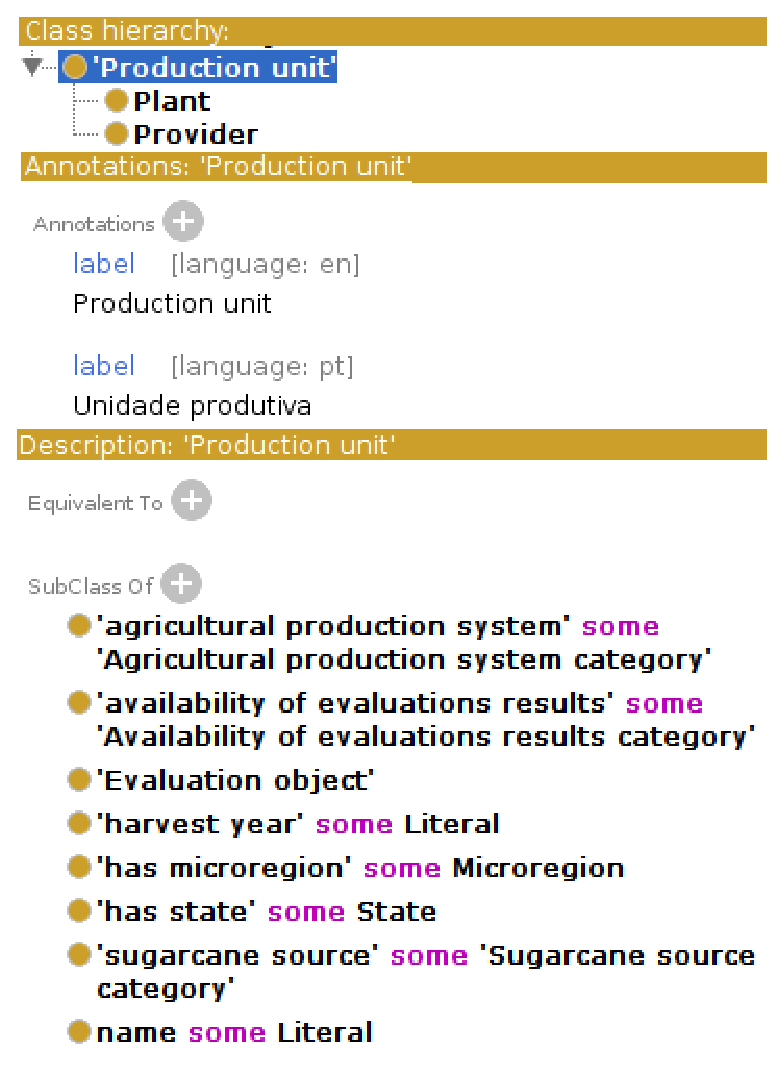
\includegraphics[width=0.6\columnwidth]{figures/ProductionUnit}
\par\end{centering}
\caption{Modelagem da classe de unidade produtiva (ProductionUnity). \label{fig:Modelagem-unidade-produtiva}}
\end{figure}

\selectlanguage{english}%

\subsection*{\textit{Microregion}\foreignlanguage{brazil}{\textit{ }}}

\selectlanguage{brazil}%
Representam os locais onde são localizadas as unidades produtivas.
É permitido definir a microrregião onde as fazendas e usinas do sistema
produtivo de cana-de-açúcar se localizam. Atualmente, a ontologia
tem os 7 estados pertencentes ao centro-sul do Brasil e as 243 microrregiões
dentro desses estados. Esses dados foram originalmente obtidos por
consulta SPARQL à DB-pedia e integrados à ontologia.

A Figura \ref{fig:Modelagem-de-Microrregi=0000E3o} mostra a modelagem
das localizações geográficas usadas no sistema SustenAgro, com algumas
instâncias de \foreignlanguage{english}{\textit{Microregion}}.

\begin{figure}[H]
\noindent \begin{centering}
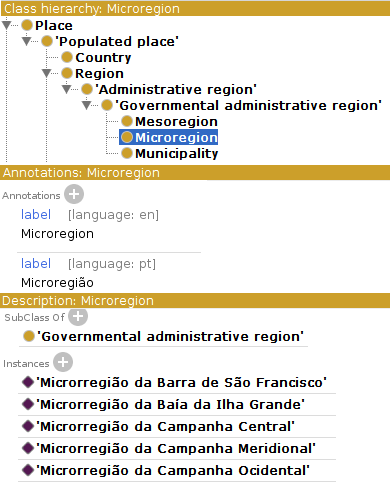
\includegraphics[width=0.6\columnwidth]{figures/Microregion}
\par\end{centering}
\caption{Modelagem de microrregiões.\label{fig:Modelagem-de-Microrregi=0000E3o}}
\end{figure}

\selectlanguage{english}%

\subsection*{\textit{Indicator}}

\selectlanguage{brazil}%
Os indicadores são o principal componente da ontologia. Eles foram
propostos por um grupo de especialistas de diversas áreas da produção
agrícola e sustentabilidade \citep{oliveira:2013}. 

Eles representam as características das unidades produtivas que serão
identificadas e quantificadas em cada processo de avaliação. Eles
tem uma propriedade \foreignlanguage{english}{\textit{Value}}\textit{
}que quantifica a sustentabilidade do indicador.

Também permite a integração de conceitos, inclusive quando pertencem
a domínios sem relação aparente. Um exemplo disso é a inter-relação
do conhecimento de sustentabilidade com conhecimento de interfaces
gráficas de usuário, que suporta a geração de SAD para avaliação da
sustentabilidade. O conhecimento foi dividido em duas ontologias,
avaliação de sustentabilidade e outra dos componentes gerais de um
SAD.

A Figura \ref{fig:Modelagem-de-Indicador} apresenta a hierarquia
dos indicadores, que está subdividida em \foreignlanguage{english}{Efficiency
Indicator} e \foreignlanguage{english}{Sustainability Indicator}.
Os \foreignlanguage{english}{Indicators} têm a propriedade \foreignlanguage{english}{\textit{has
value}}\textit{ }que estabelece um valor\textit{ .} Existe outra
propriedade, \foreignlanguage{english}{has weight,} que é opcional
e estabelece um peso para o indicador\foreignlanguage{english}{\textit{.}}

A Figura \ref{fig:Modelagem-de-Indicador} mostra o indicador intitulado
\foreignlanguage{english}{\textit{Adequacy of boilers}}. Na propriedade
\foreignlanguage{english}{\textit{has value}} ele tem uma restrição
que limita os valores dessa propriedade a valores de uma lista de
valores categóricos. A propriedade \foreignlanguage{english}{\textit{has
weight}} também tem uma restrição que limita seus valores a instâncias
da classe \foreignlanguage{english}{\textit{Sugarcane process Optimization}}.

\begin{figure}[H]
\noindent \begin{centering}
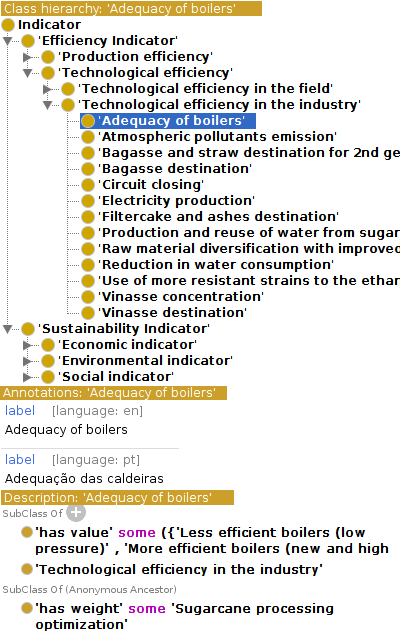
\includegraphics[width=0.6\columnwidth]{figures/Indicador}
\par\end{centering}
\caption{Modelagem de indicador \label{fig:Modelagem-de-Indicador}}
\end{figure}

Segundo a descrição do método de avaliação (Capítulo \ref{chap:Sustainability_Assessment}),
os indicadores de sustentabilidade são classificados em três dimensões
de sustentabilidade: dimensão ambiental, dimensão social e dimensão
econômica. Tendo as três uma participação equitativa no método de
avaliação \citep{kraines2011system}. 

A Figura \ref{fig:environment} representa a dimensão de indicadores
ambientais, de onde foram definidos os seguintes conceitos:

\begin{figure}[H]
\begin{centering}
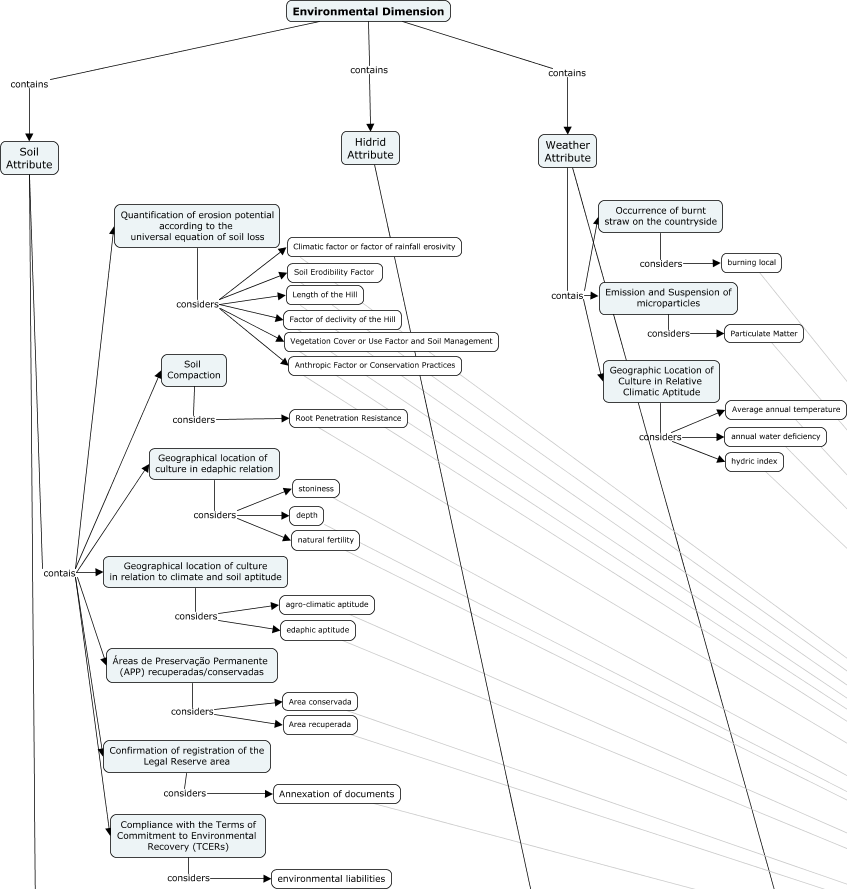
\includegraphics[width=1\textwidth]{figures/ambiental}
\par\end{centering}
\caption{Mapa conceitual - Dimensão Ambiental.\label{fig:environment}}
\end{figure}

\begin{itemize}
\item Atributo solo (\foreignlanguage{english}{Soil Attribute}): indicadores
que avaliam os aspectos referentes às características do solo.
\item Atributo hídrico (\foreignlanguage{english}{Hydric Attribute}): indicadores
que avaliam os aspectos referentes à disponibilidade e qualidade das
fontes hídricas.
\item Atributo clima (\foreignlanguage{english}{Weather Attribute}): indicadores
que avaliam os aspectos climáticos.
\end{itemize}
Nessa dimensão (ambiental), não foi possível identificar indicadores
de tipo hídrico. Não existe consenso entre os especialistas consultados
sobre quais são os aspectos mais relevantes deles para a avaliação
da sustentabilidade, porém, é um aspecto fundamental para trabalhar
nas futuras etapas de pesquisa.

A Figura \ref{fig:social} mostra a dimensão social, onde são definidos
os seguintes conceitos:

\begin{figure}[H]
\centering{}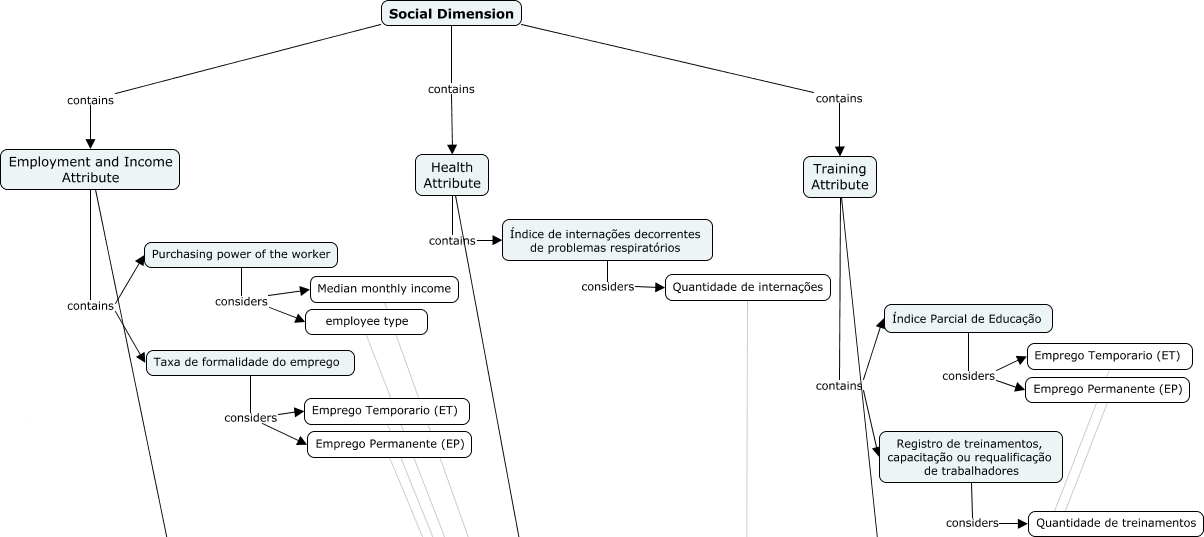
\includegraphics[width=1\textwidth]{figures/social}\caption{Mapa conceitual - Dimensão Social.\label{fig:social}}
\end{figure}

\begin{itemize}
\item Atributo emprego e renda (\foreignlanguage{english}{Employment and
Income Attribute}): indicadores que avaliam os aspectos referentes
à mão de obra.
\item Atributo saúde (\foreignlanguage{english}{Health Attribute}): indicadores
que avaliam os aspectos de segurança dos trabalhadores.
\item Atributo treinamento (\foreignlanguage{english}{Training Attribute}):
indicadores que avaliam os aspectos da capacitação dos trabalhadores.
\end{itemize}
Nessa dimensão (Social), é importante reconhecer que as unidades produtivas,
sejam do tipo fazendas ou usinas, têm vínculos com pessoas tanto internamente
como externamente. Por isso, é importante refinar os indicadores para
incluir a população externa à unidade produtiva que é afetada pelas
práticas produtivas.

A Agência Paulista de Tecnologia dos Agronegócios (APTA\nomenclature{APTA}{Agência Paulista de Tecnologia dos Agronegócios})
forneceu dados econômicos das principais usinas do estado de São Paulo,
que permitiram definir a dimensão econômica das unidades produtivas
na ontologia de domínio.

As Figuras \ref{fig:Economic-1} e \ref{fig:Economic-2} apresentam
a dimensão econômica, onde foram definidos os seguintes conceitos:

\begin{figure}[H]
\begin{centering}
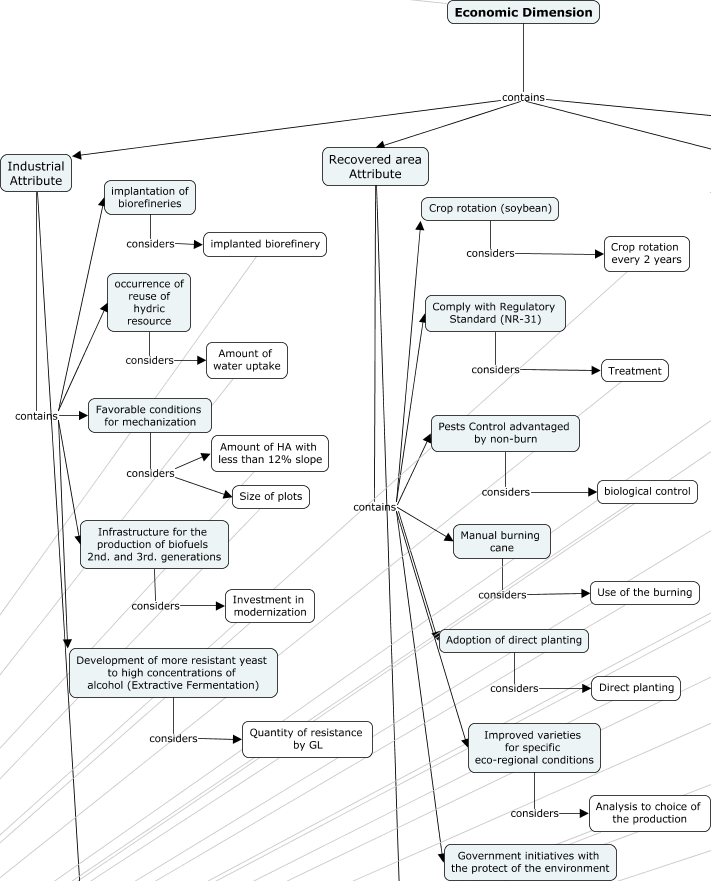
\includegraphics[width=1\textwidth]{figures/economica_1}
\par\end{centering}
\caption{Mapa conceitual - Dimensão Econômica (primeira parte).\label{fig:Economic-1}}
\end{figure}

\begin{figure}[H]
\begin{centering}
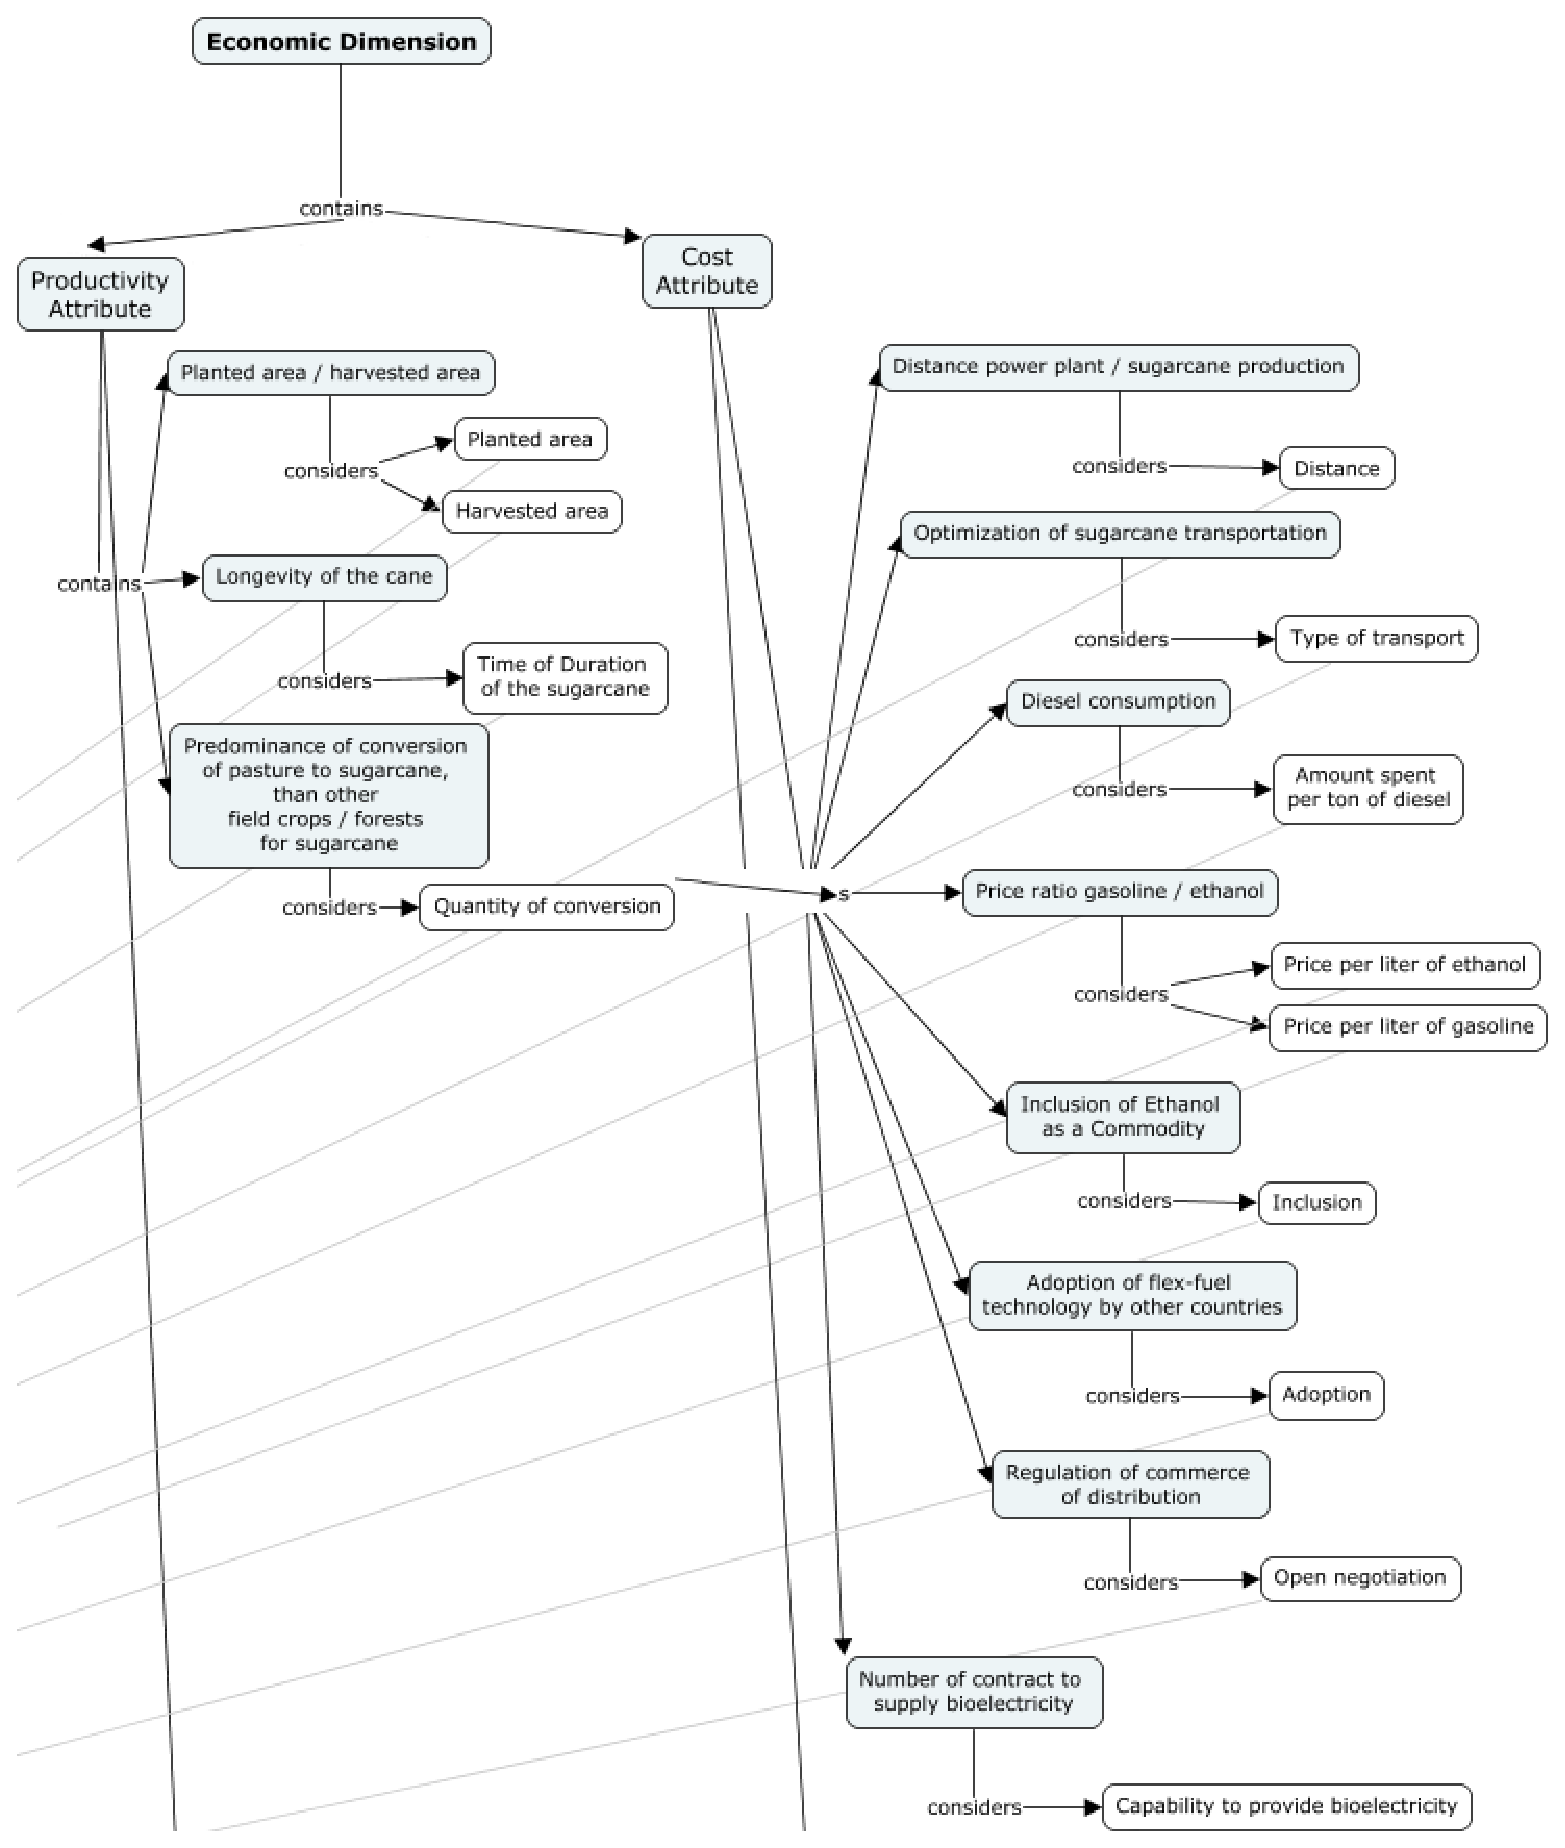
\includegraphics[width=1\textwidth]{figures/economica_2}
\par\end{centering}
\caption{Mapa conceitual - Dimensão Econômica (segunda parte).\label{fig:Economic-2}}
\end{figure}

\begin{itemize}
\item Atributo industrial (Industrial Atribute): indicadores que avaliam
os aspectos industriais. 
\item Atributo área recuperada (Recovered Area Atribute): indicadores que
avaliam os aspectos da área produtiva e das técnicas produtivas.
\item Atributo produtividade (Porductivity Atribute): indicadores que avaliam
os aspectos dos produtos e dos processos produtivos.
\item Atributo custo (Cost Atribute): indicadores que avaliam os aspectos
dos custos da produção. 
\end{itemize}
Cada uma das três dimensões deve ser avaliada equitativamente para
gerar um resultado coerente com a teoria da sustentabilidade agrícola\citep{tilman2002agricultural}.
A Figura \ref{fig:Method} mostra os conceitos envolvidos na avaliação
da sustentabilidade, fazendo uma integração entre os indicadores e
o método de avaliação. Cada um dos indicadores tem componentes de
indicadores que serão processados pelo método de avaliação, permitindo
quantificar a sustentabilidade.

\begin{figure}[H]
\begin{centering}
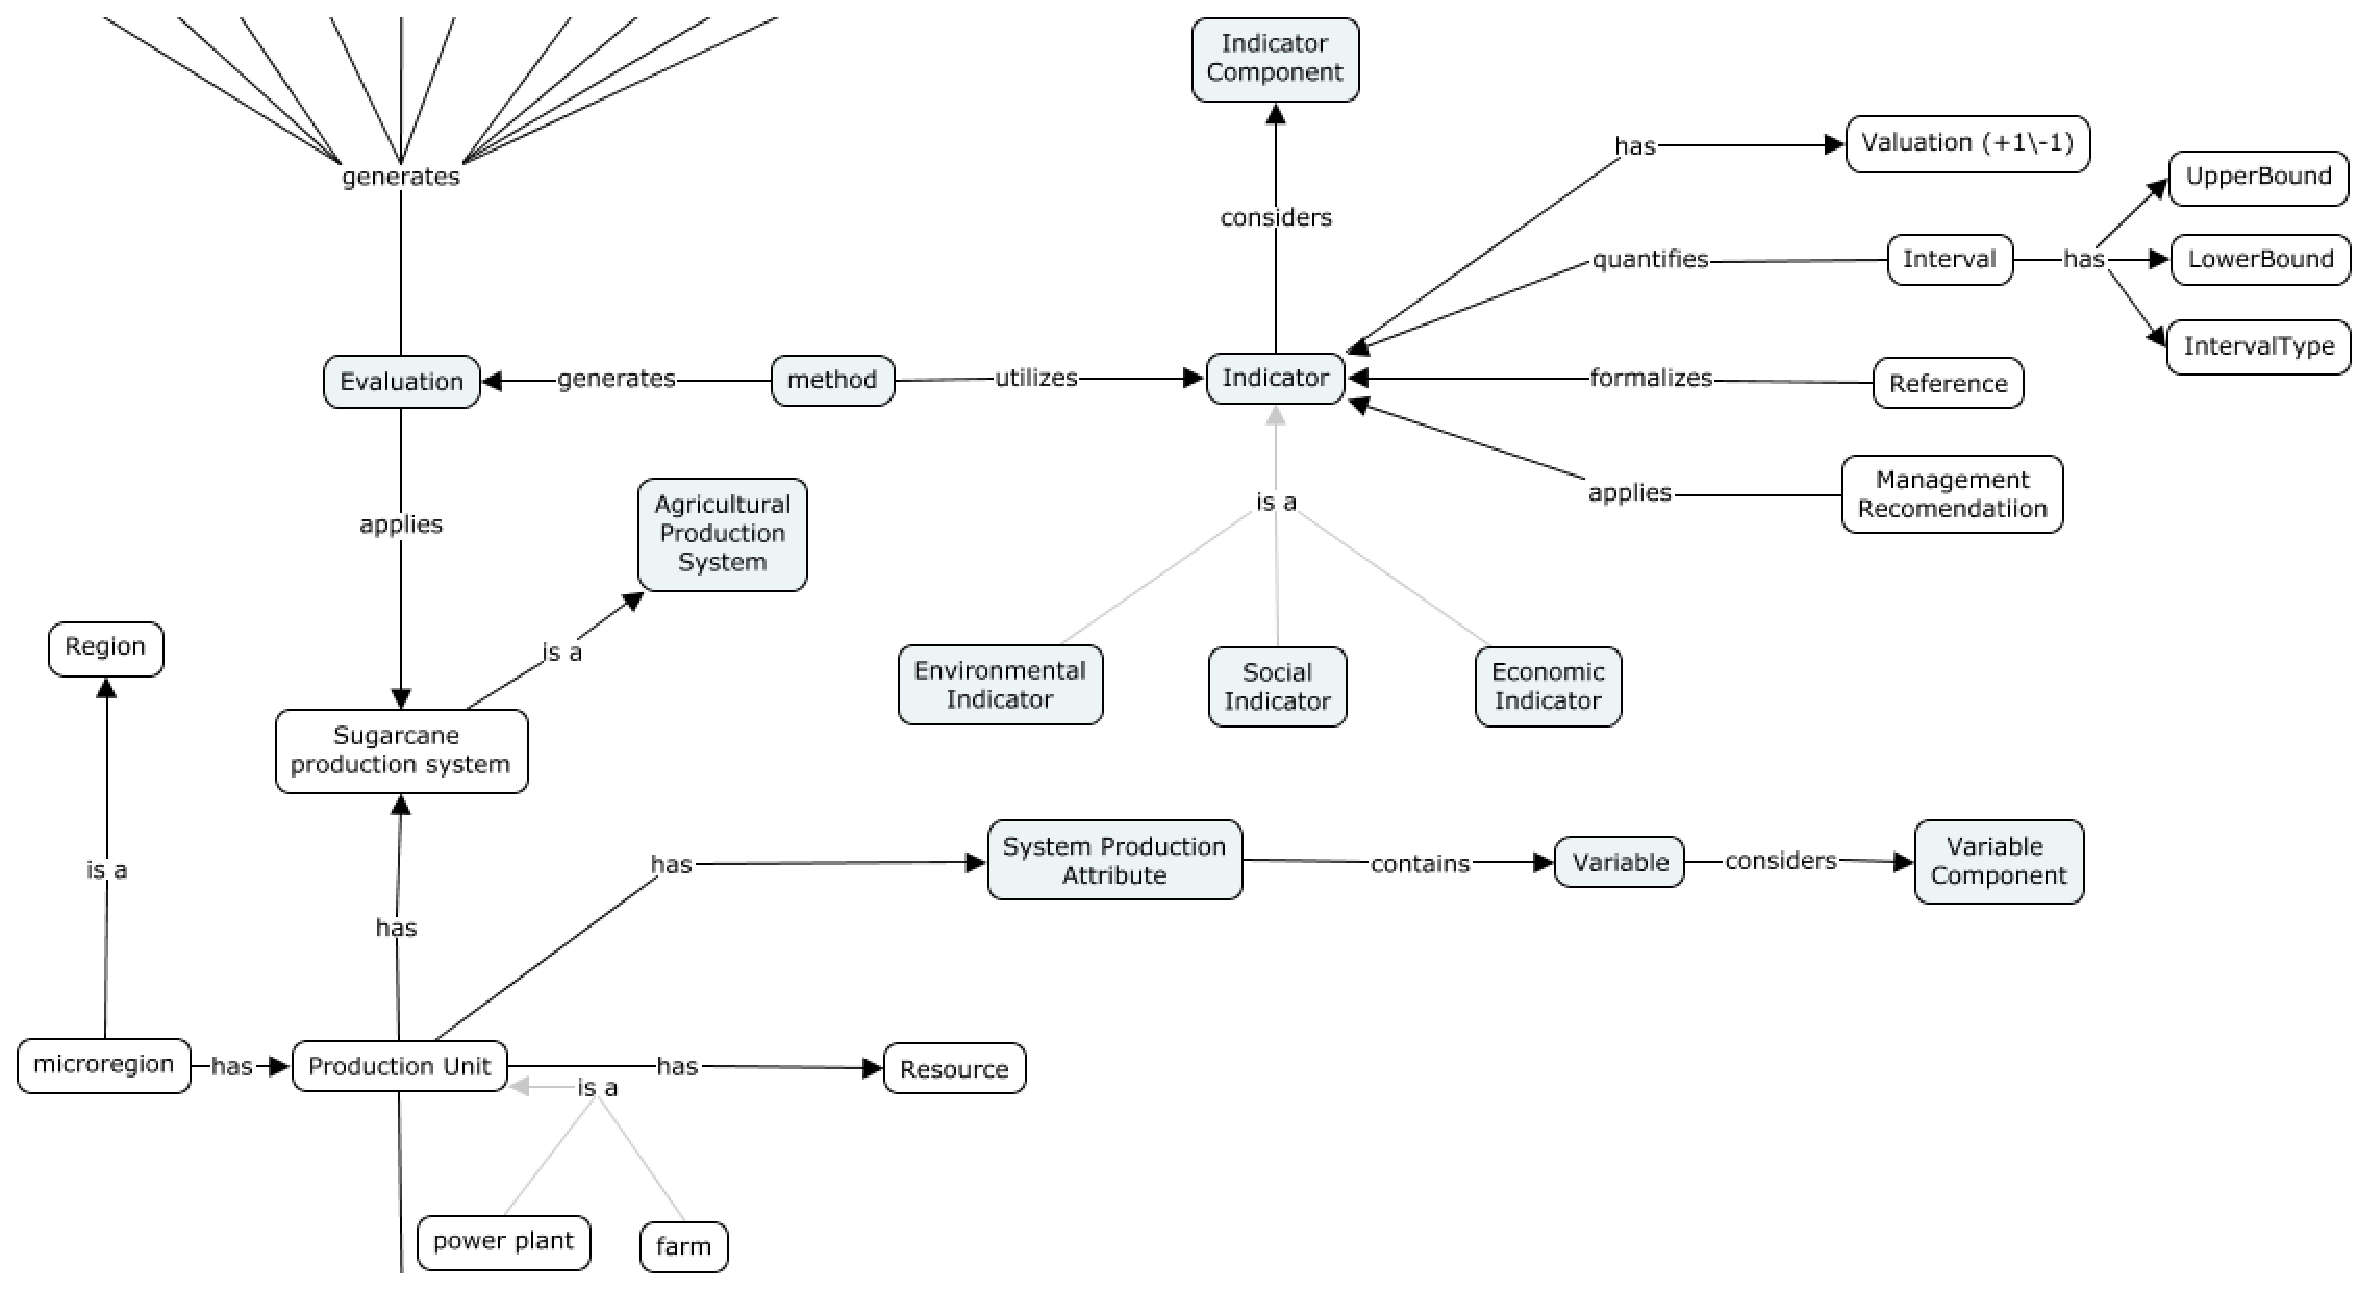
\includegraphics[width=1\textwidth]{figures/metodo}
\par\end{centering}
\caption{Mapa conceitual - Método de Avaliação.\label{fig:Method}}
\end{figure}

As dimensões da sustentabilidade permitiram organizar os indicadores,
levando essa organização desde os modelos de mapas conceituais, às
ontologias, método de avaliação e, finalmente, até a representação
dos resultados nas web UI dos SADs.
\selectlanguage{english}%

\subsection*{Categorical}

\selectlanguage{brazil}%
O conceito \foreignlanguage{english}{Categorical} representa os possíveis
\foreignlanguage{english}{Value} que um \foreignlanguage{english}{\textit{Indicator}}
ou \foreignlanguage{english}{\textit{Variable}} pode ter na forma
de categorias (por exemplo, Existe e Não Existe). Um Value também
pode ser Real ou Inteiro. Na verdade, a classe Categorical é definida
na ontologia Decisioner, mas a SustenAgro cria diversas classes filhas
para definir uma série de valores categóricos.

Cada subclasse de Categorical é composta por um conjunto finito de
elementos ou valores. Cada valor é modelado como indivíduo da classe,
permitindo assim, restringir as opções de instanciação de cada indicador.

Na Figura \ref{fig:Modelagem-de-Value}, é apresentada a classe \foreignlanguage{english}{\textit{Value}}
e suas subclasses, tanto \foreignlanguage{english}{\textit{Categorical}}
para conjunto finito de valores e \foreignlanguage{english}{\textit{Real}}
para valores numéricos. Um exemplo de classe categórica seria a \foreignlanguage{english}{\textit{Yes/No}}
que representa os valores de sim e não e é composta pela lista de
indivíduos Yes e No.

Cada individuo da classe \foreignlanguage{english}{\textit{Value}}
tem a propriedade \foreignlanguage{english}{\textit{as number}}\textit{
}que relaciona a ele um valor numérico. Esse valor define um critério
de comparação entre os indivíduos da mesma classe. Ele é usado nas
fórmulas do método de avaliação.

\begin{figure}[H]
\begin{centering}
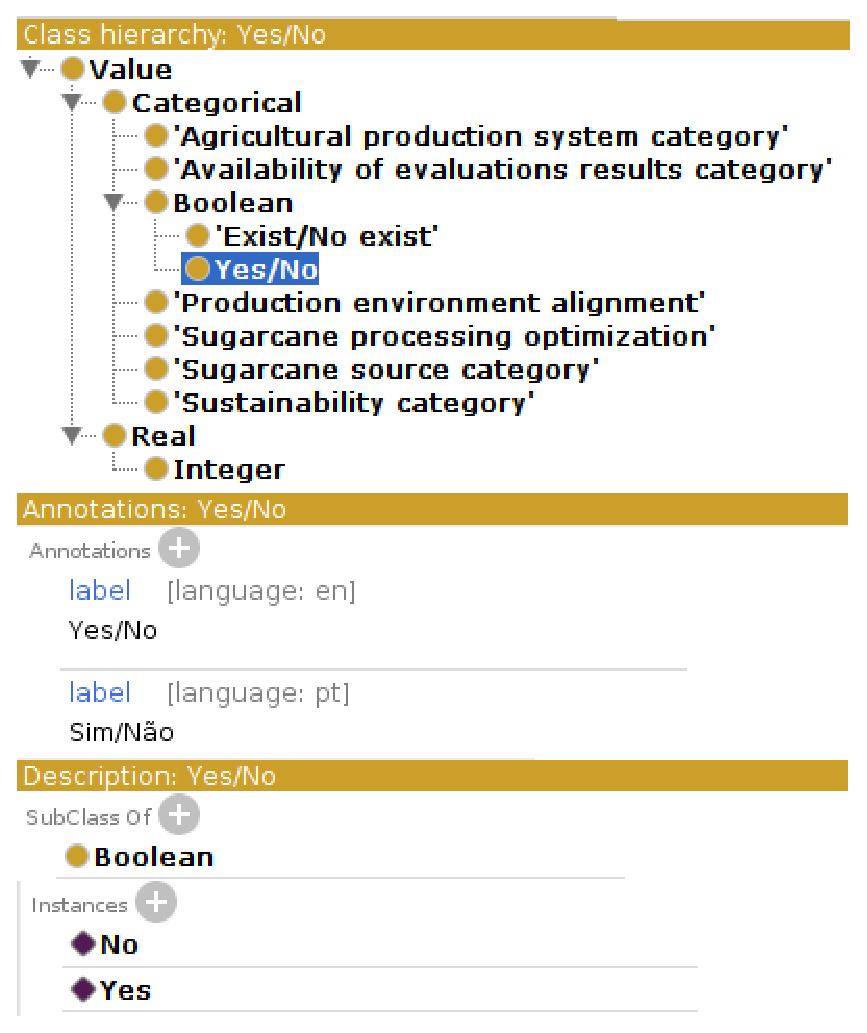
\includegraphics[scale=0.6]{figures/Value}
\par\end{centering}
\caption{Modelagem de \foreignlanguage{english}{Value}\label{fig:Modelagem-de-Value}}
\end{figure}

\selectlanguage{english}%

\section{SustenAgro Web UI\label{sec:Web-UI}}

\selectlanguage{brazil}%
O design das interfaces gráficas e desenvolvimento dos web componentes
foram realizados por meio da várias técnicas de levantamento de requerimentos
para especificar as funcionalidades que os especialistas precisavam
do sistema SustenAgro. Foram usadas as seguintes técnicas: \foreignlanguage{english}{User
Stories}, \foreignlanguage{english}{Scenarios}, \foreignlanguage{english}{Storyboard},
\foreignlanguage{english}{Mockups} e protótipo de interface gráfica.

Na fase inicial, foram definidos os perfis de usuários do SAD SustenAgro,
inicialmente definiram-se os perfis descritos a seguir: 
\begin{itemize}
\item Administrador: usuário com permissões para editar Ontologias, DSL
e web UI. Ele é o responsável pela administração do SAD e tem todas
as permissões do sistema.
\item Especialista de domínio: especialista em sustentabilidade ou afins,
com permissões para recuperar e gerenciar informações das avaliações,
gerar reportes e mudar os conceitos relacionados com os indicadores
e método de avaliação.
\item Usuário final: usuário padrão do sistema que tem permissões para realizar
avaliações de sustentabilidade em cana-de-açúcar e de gerenciar os
dados cadastrados por ele. 
\end{itemize}
No SAD SustenAgro v1.0, foi removido o perfil especialista, ficando
apenas os perfis administrador e usuário final. As funções desse perfil
foram incluídas no perfil administrador.

As técnicas realizadas para desenvolver as web UI, são descritas a
seguir.
\selectlanguage{english}%

\subsection*{User Stories}

\selectlanguage{brazil}%
Histórias de usuário são uma técnica para descrever, de uma forma
curta e simples, as características do sistema a partir da perspectiva
do usuário ou cliente do sistema, gerando uma definição de alto nível
de um requisito. O padrão é: como um “tipo de usuário”, eu quero atingir
“algum objetivo” para “alguma finalidade”.

Na aplicação dessa técnica foram obtidas as seguintes histórias:
\begin{enumerate}
\item O usuário poderá identificar e cadastrar a localização geográfica
e a área da sua lavoura (definir região geográfica do IBGE, latitude
e longitude - a partir do \foreignlanguage{english}{Google Maps}). 
\item O usuário poderá identificar e cadastrar a microrregião a que pertence
a sua lavoura. O sistema fará uma sugestão de cadastro a partir dos
dados da localização geográfica.
\item O usuário deverá preencher o estado de cada indicador específico nas
dimensões ambiental, econômica e social, devendo adaptar-se às condições
das regiões e microrregiões do Brasil.
\item O usuário poderá obter o resultado dos índices, segundo a informação
preenchida e a fórmula de agregação dos indicadores.
\item O usuário poderá armazenar a informação dos indicadores para futuras
consultas.
\item O usuário poderá acrescentar indicadores que considere importantes
para a análise. Deve-se estabelecer regras para essa funcionalidade
de tal modo que os novos indicadores (criados pelos usuários) sejam
recuperáveis de um modo separado dos indicadores cadastrados no sistema. 
\item O sistema deve fornecer um cronograma de avaliação, sendo recomendado
realizar a avaliação depois de cada safra.
\end{enumerate}
O usuário pode empregar a metodologia de avaliação caso a caso: possibilitando
que o usuário selecione quais indicadores vai utilizar, podendo recomendar
limiares mais adequados para a realidade dele e também inserir novos
indicadores/limiares. Finalmente, o usuário deverá ser informado da
importância dos processos de avaliação, exemplo: 
\begin{itemize}
\item “A crescente demanda de países desenvolvidos por produtos com garantia
de origem tem induzido aumento das certificações nas usinas no Brasil
(ALVES et al., 2008).” 
\item A certificação tem sido uma importante forma de diferenciação de commodities
agrícolas, facilitando seu acesso aos mercados protegidos dos países
desenvolvidos. 
\item A caracterização climática, aliada aos detalhes de fertilidade e manejo
do solo (quantificação edafoclimática), são essenciais para a determinação
das regiões aptas ao cultivo de culturas de interesse comercial (CIIAGRO,
2009). 
\end{itemize}
Depois do ingresso da informação sobre os indicadores, o usuário receberá
recomendações classificadas sobre práticas de sustentabilidade recomendadas
com sua argumentação, exemplo: 
\begin{itemize}
\item (Ambiental) “O sistema de plantio direto da cana-de-açúcar sobre leguminosas
proporciona maiores teores foliares de N e K na cana do que o plantio
convencional (JÚNIOR; COELHO, 2008)”.
\item (Ambiental) Segundo Leme (2005), haveria redução de 36\% na emissão
de gases do efeito estufa (GEE) se a palha fosse queimada nas caldeiras
das usinas e destilarias, ao invés de ser queimada no campo.
\item (Ambiental) A queima da cana aumenta a erosão do solo e a poluição
do ar e reduz a qualidade da matéria-prima (LINS; SAAVEDR, 2007). 
\item (Ambiental) Quando a cana não é queimada, proliferam, nos canaviais,
roedores silvestres originários de fragmentos florestais. Esses roedores
podem transmitir o Hantavírus através da urina e contaminar cortadores
de cana, causando uma síndrome respiratória e cardíaca, a pneumocitose,
podendo levar à morte. 
\item (Ambiental) Quando não há queima da cana é comum, também, o aumento
do ataque de cigarrinhas, com perdas significativas de produção (ANDRADE;
DINIZ, 2007). 
\item (Econômico) A utilização das colheitadeiras reverte-se em aumento
da produtividade e da qualidade da matéria-prima, bem como em diminuição
dos custos da produção agrícola, que representam entre 50\% e 60\%
em relação ao custo total (SCOPINHO, 1995).
\item (Econômico e Social) A utilização das colheitadeiras em cooperativa
possibilita a soma das áreas de produtores próximos possibilitando
a mecanização em propriedades com restrição para mecanização.
\item (Econômico) Restrições físicas da propriedade (menos de 500 ha de
área com declividade inferior a 12\% e talhões menores que 800 metros)
dificultam a mecanização. 
\end{itemize}
\selectlanguage{english}%

\subsection*{Scenarios}

\selectlanguage{brazil}%
É uma técnica que permite a descrição das funcionalidades do sistema
desde a perspectiva do usuário ou cliente, realizando uma descrição
detalhada de cada um dos passos dos usuários no sistema para completar
uma tarefa. A seguir serão apresentadas as 8 histórias de usuários
do SAD SustenAgro com os cenários associados:

\textbf{História de usuário \#1:} “O usuário poderá identificar e
cadastrar a localização geográfica e a área da sua lavoura (definir
região geográfica do IBGE, latitude e longitude - a partir do \foreignlanguage{english}{Google
Maps}).”
\begin{enumerate}
\item O usuário ingressa na conta dele, através do sistema web SustenAgro
em \url{http://sustenagro.embrapa.br}, e o sistema apresenta a tela
“\foreignlanguage{english}{Home}” 
\item O usuário seleciona a aba “unidades produtivas” e dá um \foreignlanguage{english}{click}
em ``cadastrar unidade produtiva'', o sistema apresenta a tela de
cadastro de unidades produtivas, onde tem um mapa do \foreignlanguage{english}{Google
Maps} 
\item O usuário seleciona no mapa um ponto que identificará a localização
da unidade produtiva, se ele quiser, também é possível marcar a área
da lavoura para que o sistema possa ter dados mais específicos para
o processo de avaliação de sustentabilidade. Uma vez terminado, o
usuário dá um \foreignlanguage{english}{click} no botão “próximo”
e o sistema cadastra a informação preenchida. 
\end{enumerate}
\textbf{História de usuário \#2}: “O usuário poderá identificar e
cadastrar a microrregião a que pertence a unidade produtiva dele,
por meio de uma sugestão que o sistema faz com os dados da localização
geográfica.”
\begin{enumerate}
\item O usuário poderá fazer a “Historia de usuário \#1” ou entrar no sistema
e continuar com o cadastro da unidade produtiva de onde ele tenha
parado. O sistema apresentará uma tela com sugestões de microrregiões. 
\item O usuário poderá escolher a microrregião, onde esteja localizada a
unidade produtiva, e salvá-la no sistema por meio do botão ``próximo''. 
\end{enumerate}
\textbf{História de usuário \#3:} “O usuário deverá preencher o estado
de cada indicador específico nas dimensões ambiental, econômica e
social. Esses indicadores devem adaptar-se às condições das regiões
e microrregiões do Brasil, da mesma forma as faixas de limiares de
sustentabilidade foram definidas.''
\begin{enumerate}
\item O usuário poderá fazer a “História de usuário \#2” ou entrar no sistema
e continuar com o cadastro dos indicadores de onde ele tenha parado.
O sistema apresentará uma tela com três abas que contém os controles
que permitirão fazer o cadastro dos indicadores nas dimensões ambiental,
econômica e social. 
\item O usuário dá um \foreignlanguage{english}{click} na primeira aba e
começa a preencher os dados dos indicadores ambientais, principalmente
os limiares que identificam o estado do indicador. A interface também
permite eliminar ou acrescentar indicadores específicos, por parte
dos usuários (funcionalidade que é explicada na “Hstória de usuário
\#4”). 
\item O usuário preenche os dados das outras duas dimensões e o sistema
salva as mudanças.
\end{enumerate}
\textbf{História de usuário \#4:} “Permitir o emprego da metodologia
para avaliação caso a caso: possibilitar que o usuário selecione quais
indicadores vai utilizar. Dentro dos indicadores, ele pode recomendar
limiares mais adequados para a sua realidade, também pode inserir
novos indicadores\slash{}limiares.”
\begin{enumerate}
\item O usuário poderá fazer a “Historia de usuário \#3” ou entrar no sistema
e continuar na tela de cadastro de indicadores e, quando aconteçer
que o usuário precise de um indicador que não seja oferecido pelo
sistema, o usuário poderá acrescentá-lo por meio do botão “acrescentar
indicador” 
\item O usuário dá um \foreignlanguage{english}{click} no botão “acrescentar
indicador” e lhe é apresentada uma interface de entrada, onde ele
deverá cadastrar o título, a descrição, os limiares, a medida do manejo
e a justificativa desse indicador. Em seguida preencher o estado do
indicador. O sistema salva esses dados nessa dimensão. 
\item O usuário também poderá eliminar alguns indicadores segundo seu critério.
\end{enumerate}
\textbf{História de usuário \#5:} \textquotedbl{}O usuário poderá
obter o resultado dos índices segundo a informação preenchida e a
formula de agregação dos indicadores.\textquotedbl{}
\begin{enumerate}
\item Depois de terminada a “História de usuário \#4”, o sistema fará a
avaliação, que foi definida no sistema pelos especialistas. 
\item O resultado da avaliação será cadastrado no sistema com informações
sobre a metodologia utilizada.
\item A metodologia de avaliação pode ser atualizada pelos administradores
para uso em avaliações futuras.
\end{enumerate}
\textbf{História de usuário \#6:} ``O usuário poderá armazenar a
informação dos indicadores para futuras consultas.''
\begin{enumerate}
\item O usuário preenche alguns indicadores nos formulários do SustenAgro. 
\item Esses dados serão salvos quando o usuário mudar de formulário ou quando
der um \foreignlanguage{english}{click} no botão ``próximo''.
\end{enumerate}
\textbf{História de usuário \#7:} ``O usuário poderá acrescentar
indicadores que considere importantes para sua análise, devem-se estabelecer
regras para essa funcionalidade de tal modo que os novos indicadores
(criados pelos usuários) sejam recuperáveis de um modo separado dos
indicadores cadastrados no sistema.''
\begin{enumerate}
\item Quando o usuário estiver preenchendo os indicadores gerados pelo sistema,
o sistema fornecerá um conjunto de controles que permitam a inclusão
de um novo indicador. Esse novo indicador será definido pelo próprio
usuário baseado na sua experiência na área. 
\item O sistema armazenará esse novo indicador com uma classificação especial
que permita sua identificação e separação dos outros indicadores. 
\item O usuário poderá preencher os dados do novo indicador, para que sejam
inclusos na avaliação de sustentabilidade.
\end{enumerate}
\textbf{História de usuário \#8:} ``Cronograma de avaliação, depois
de cada safra.''
\begin{enumerate}
\item Depois de fazer o cadastro da fazenda e das culturas que são plantadas
nela, o sistema poderá identificar quando termina cada safra, gerando
um alerta para que o usuário faça o processo de avaliação nessa data.
\item O usuário lerá o alerta e poderá fazer o processo de avaliação de
sustentabilidade. 
\end{enumerate}
\selectlanguage{english}%

\subsection*{Storyboard}

Storyboards\foreignlanguage{brazil}{ são similares aos cenários. Elas
ilustram a interação necessária para atingir um objetivo sem utilizar
uma lista de passos. A interação é visualizada por meio de uma história
em quadrinhos.}

\selectlanguage{brazil}%
Essa representação permite uma visão holística da interação do usuário,
com ênfase nos aspectos funcionais da interação e não nos aspectos
da interface de usuário. A seguir, são apresentados os textos das
\foreignlanguage{english}{storyboard} dos processos identificados:

A Figura \ref{fig:StoryBoard-1} apresenta o processo de cadastro
da localização da unidade produtiva, para conseguir vincular dados
a partir da localização geográfica.

\begin{figure}[H]
\begin{centering}
\includegraphics[width=1\columnwidth]{\string"figures/Stroyboard 1\string".eps}
\par\end{centering}
\centering{}\caption{\textit{\emph{\small{}StoryBoard definição da localização. \label{fig:StoryBoard-1}}}}
\end{figure}

A Figura \ref{fig:StoryBoard-2} apresenta o formulário de seleção
da microrregião que faz parte da localização descrita no \foreignlanguage{english}{storyboard}
anterior. Essa informação é importante para caracterizar a unidade
produtiva.

\begin{figure}[H]
\begin{centering}
\includegraphics[width=1\columnwidth]{\string"figures/Stroyboard 2\string".eps}
\par\end{centering}
\caption{\textit{\emph{\small{}StoryBoard seleção da unidade produtiva. \label{fig:StoryBoard-2}}}}

\end{figure}

A Figura \ref{fig:StoryBoard-3} apresenta o esquema do formulário
de preenchimento dos indicadores que permite cadastrar uma avaliação,
dito formulário é adaptável a vários tipos de dados dos indicadores,
permitindo construir interfaces amigáveis para os usuários.

\begin{figure}[H]

\includegraphics[width=1\columnwidth]{\string"figures/Stroyboard 3\string".eps}

\caption{\textit{\emph{\small{}StoryBoard mostrando o preenchimento dos indicadores.\label{fig:StoryBoard-3}}}}

\end{figure}
A Figura \ref{fig:StoryBoard-4} apresenta o processo de avaliação
para uma unidade produtiva, segundo o método Sustenagro. Ele vai processar
os indicadores preenchidos para gerar uma análise.

\begin{figure}[H]
\begin{centering}
\includegraphics[width=1\columnwidth]{\string"figures/Stroyboard 4\string".eps}
\par\end{centering}
\caption{\textit{\emph{\small{}StoryBoard}} sobre a avaliação de unidade produtiva\label{fig:StoryBoard-4}}
\end{figure}

A Figura \ref{fig:StoryBoard-5} apresenta o formulário de definição
de novos indicadores, por parte dos usuários do sistema. Eles permitem
a integração de novos conceitos ao sistema. 

\begin{figure}[H]
\begin{centering}
\includegraphics[width=1\columnwidth]{\string"figures/Stroyboard 6\string".eps}
\par\end{centering}
\centering{}\caption{\textit{\emph{\small{}StoryBoard}} para cadastro de novo indicador.\label{fig:StoryBoard-5}}
\end{figure}

A Figura \ref{fig:StoryBoard-6} apresenta o relatório resultante
do processo de avaliação. Ele é composto pelos índices, uma tabela
dos dados cadastrados , a matriz de sustentabilidade e as recomendações

\begin{figure}[H]
\begin{centering}
\includegraphics[width=1\columnwidth]{\string"figures/Stroyboard 5\string".eps}
\par\end{centering}
\caption{\textit{\emph{\small{}StoryBoard}} mostrando a apresentação de resultados\label{fig:StoryBoard-6}}
\end{figure}


\subsection*{Mockups das Interfaces do SustenAgro}

Estes Mockups permitiram criar uma representação visual das interfaces
do sistema, com suas \foreignlanguage{english}{widgets,} para ajudar
na sua avaliação por parte dos especialistas do domínio.  O desenvolvimento
dos \foreignlanguage{english}{mockups} foram feitos com a ferramenta
\foreignlanguage{english}{Moqups} \footnote{Moqups \url{https://moqups.com/} }.

A Figura \ref{fig:Mockup_home} mostra uma interface gráfica web do
\foreignlanguage{english}{Home}. A interface mostra uma descrição
do sistema, e as principais abas, entre elas a aba de Ferramenta que
permite iniciar o processo de avaliação de sustentabilidade.

\begin{figure}[H]
\centering{}\includegraphics[width=1\columnwidth]{\string"figures/Mockup Main\string".eps}\caption{Mockup da tela inicial do SustenAgro.\label{fig:Mockup_home}}
\end{figure}

A Figura \ref{fig:Mockup_indicators} apresenta os passos do processo
de avaliação, na ordem representada pela numeração das abas. realizando
o cadastro da localização, da cultura, das tecnologias usadas, da
caracterização do sistema produtivo, a tela dos indicadores e das
recomendações. A tela apresentada corresponde ao formulário de cadastro
dos indicadores, que permite cadastrar o valor correspondente a cada
indicador.

\begin{figure}[H]
\centering{}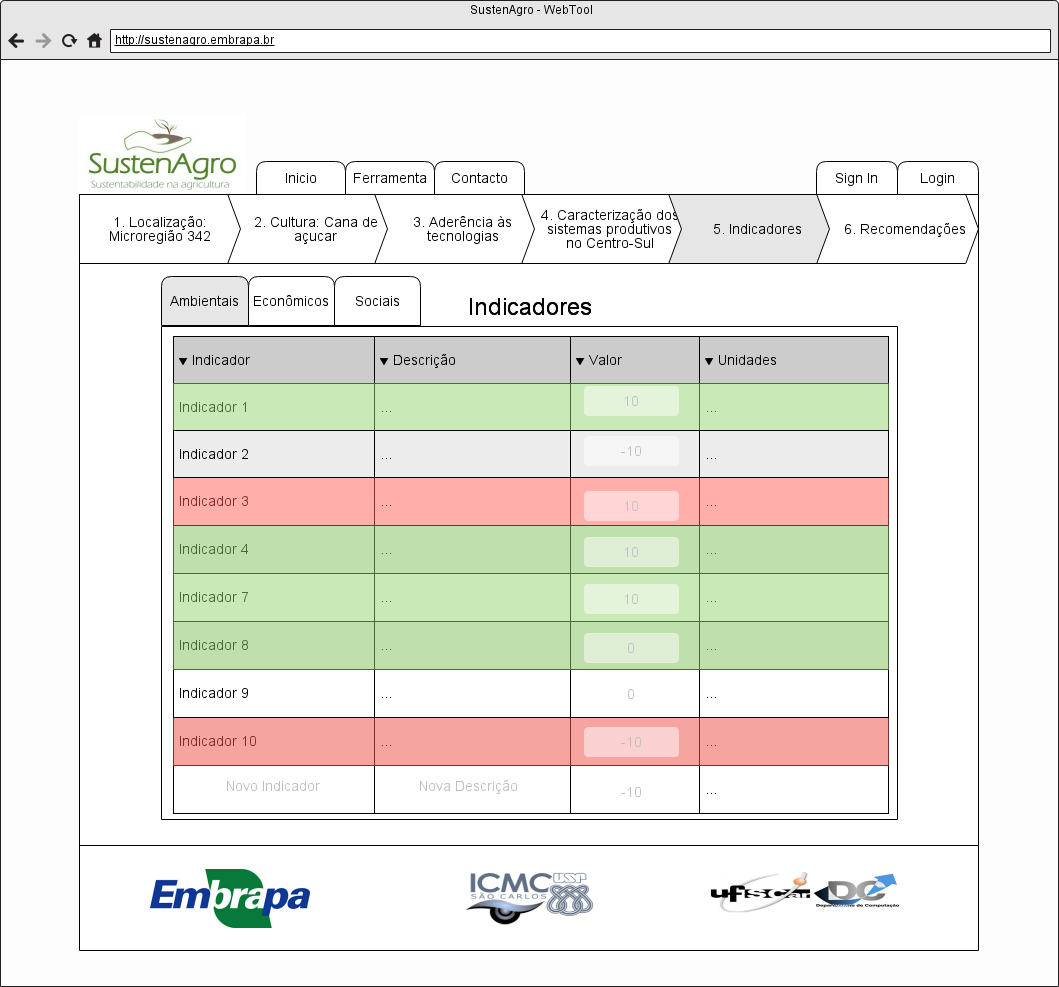
\includegraphics[width=1\columnwidth]{figures/Tool_environmental_indicators}\caption{Mockup da tela de indicadores do SustenAgro.\label{fig:Mockup_indicators}}
\end{figure}


\subsection*{Protótipo da Interface Gráfica do SustenAgro}

O protótipo funcional da interface gráfica do SustenAgro está disponível
nos servidores do laboratório Intermídia do ICMC\nobreakdash-USP
\footnote{http://biomac.icmc.usp.br:8080/sustenagro/}. Na Figura
\ref{fig:Home} é apresentada a página inicial do protótipo.

\begin{figure}[H]
\begin{centering}
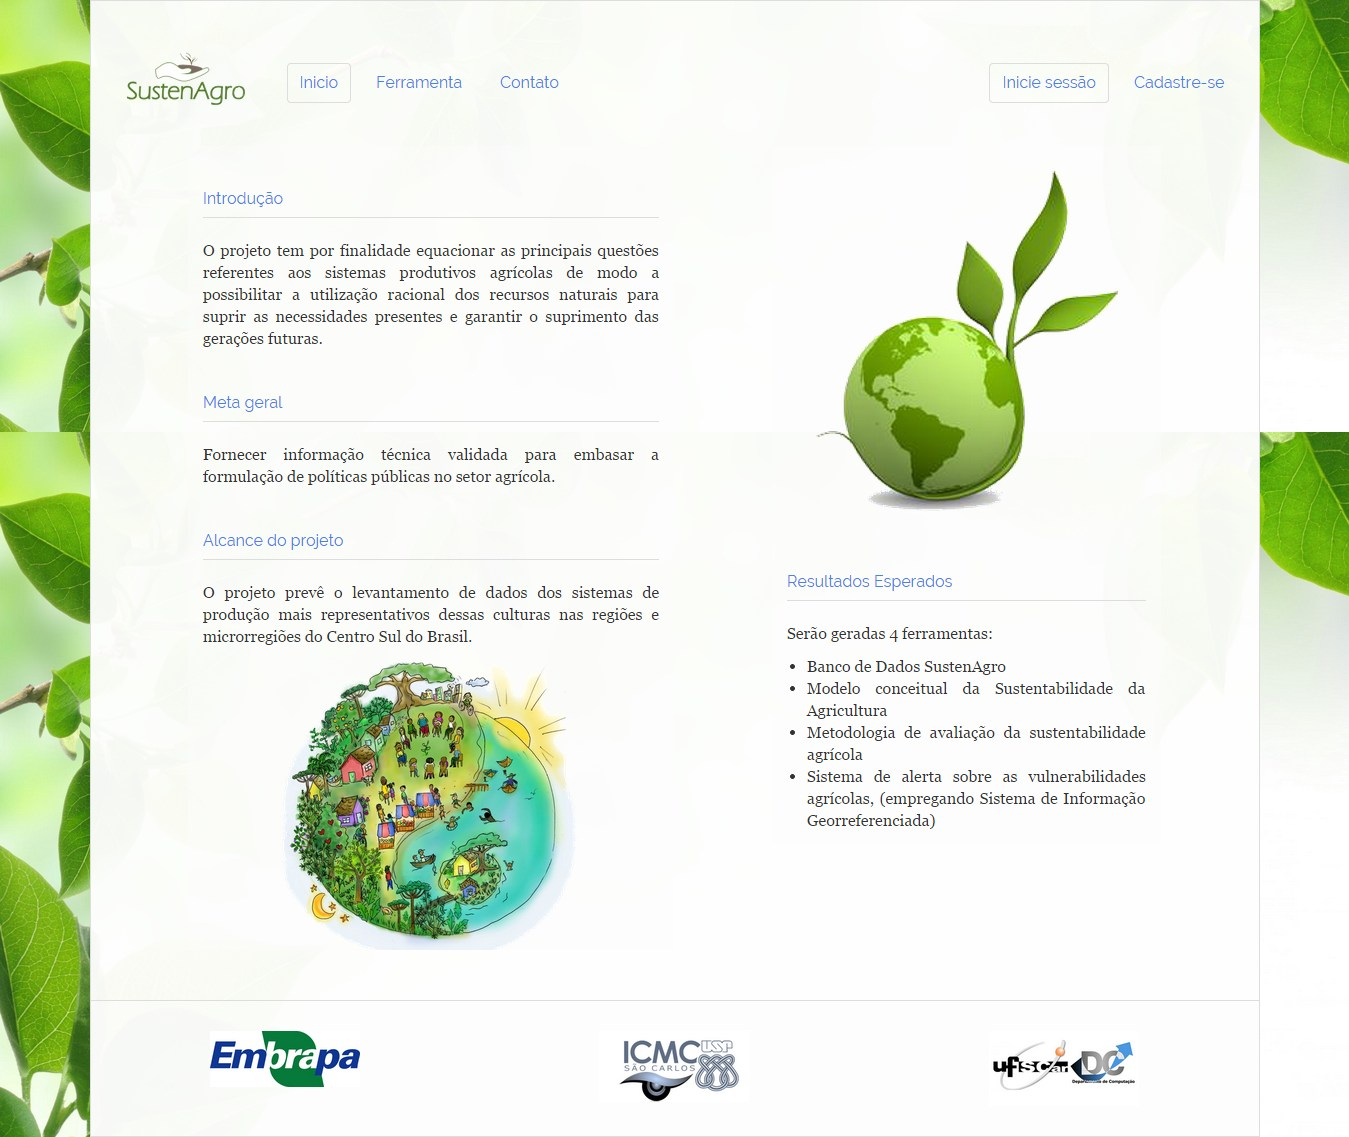
\includegraphics[width=1\textwidth]{figures/home}
\par\end{centering}
\caption{Protótipo do SustenAgro – Home Page.\label{fig:Home}}
\end{figure}

Nessa tela pode-se observar o texto explicativo da ferramenta e as
abas de ``Início'', ``Ferramenta'' e ``Contato''. A opção ``Ferramenta''
permite iniciar o processo de avaliação de sustentabilidade.

Uma vez cadastrada uma unidade produtiva, disponibiliza-se a opção
de criar nova avaliação. Essa, ação vai gerar a tela da Figura \ref{fig:Indicators},
que permite visualizar os indicadores para que os usuários preencham
cada um, segundo a realidade da unidade produtiva em avaliação. Cada
indicador tem várias opções de resposta que estão ligadas a valores
que quantificam a sustentabilidade. Esses valores estão definidos
na ontologia de sustentabilidade (a ontologia SustenAgro) e são usados
nas fórmulas para gerar os índices de sustentabilidade. 

Na Figura \ref{fig:Indicators}, é apresentado o formulário dos indicadores
de eficiência. Eles são subdivididos em eficiência de produção e tecnológica.
Na Figura \ref{fig:Indicators}, é mostrado o indicador Manejo, como
exemplo. Um tipo de manejo foi escolhido e o peso desse indicador
foi declarado como direto. Esses valores serão usados nas fórmulas
da avaliação da sustentabilidade.

\begin{figure}[H]
\noindent \begin{centering}
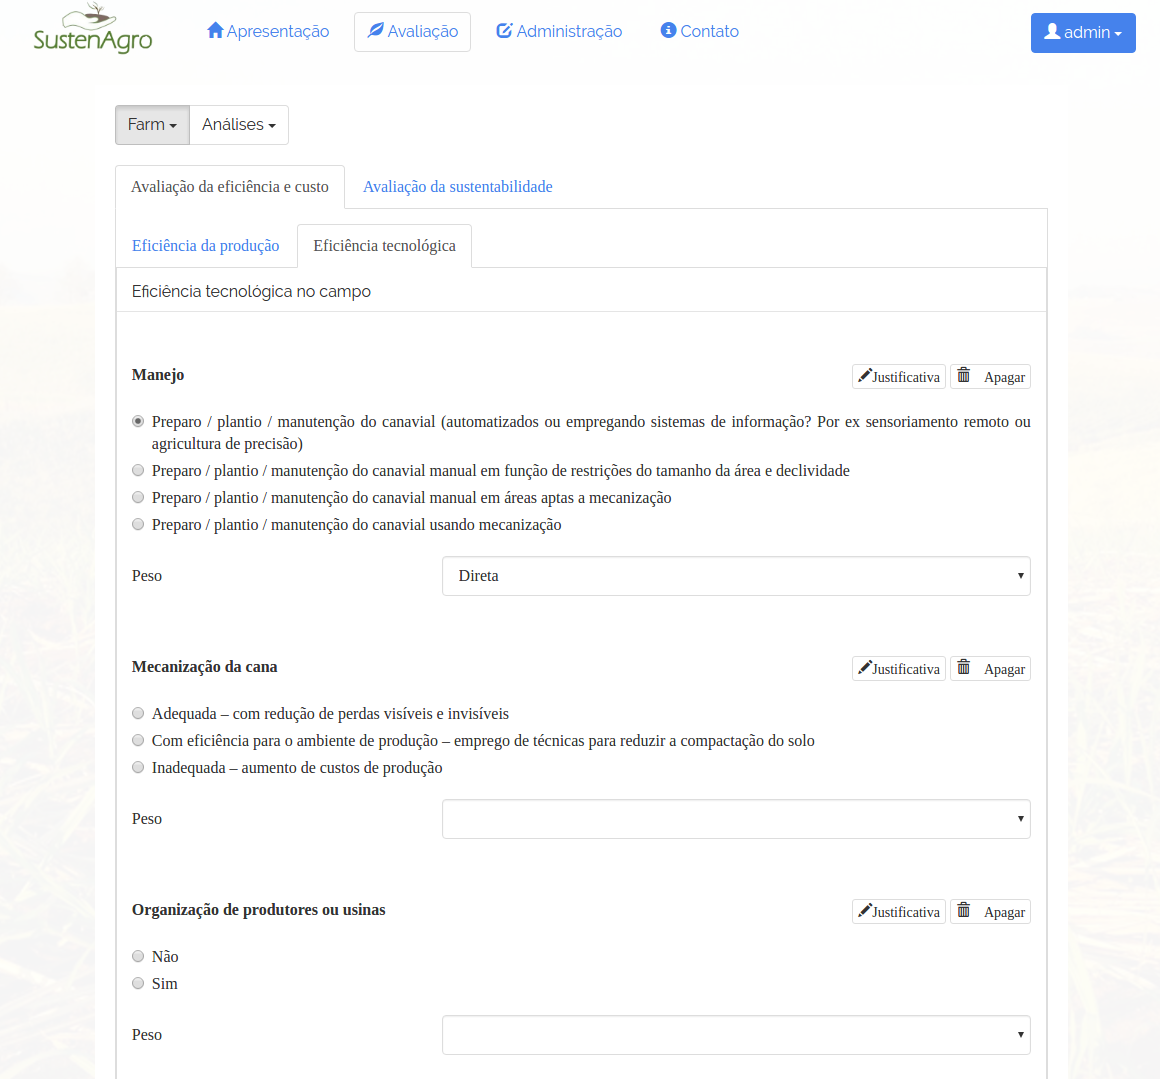
\includegraphics[width=1\columnwidth]{figures/SustenAgro-scenario}
\par\end{centering}
\caption{Cadastro de indicadores \label{fig:Indicators}}
\end{figure}

A partir dos dados cadastrados, são gerados os resultados do sistema.
Eles consistem na planilha de eficiência e custo, na planilha da sustentabilidade
e o relatório do sistema. As planilhas permitem visualizar os atributos
dos indicadores e a tela de relatório apresenta a matriz de sustentabilidade,
onde são relacionados os índices de eficiência e de sustentabilidade.
O relatório é apresentado na Figura \ref{fig:Planilhas-de-resultado}. 

\begin{figure}[H]
\noindent \begin{centering}
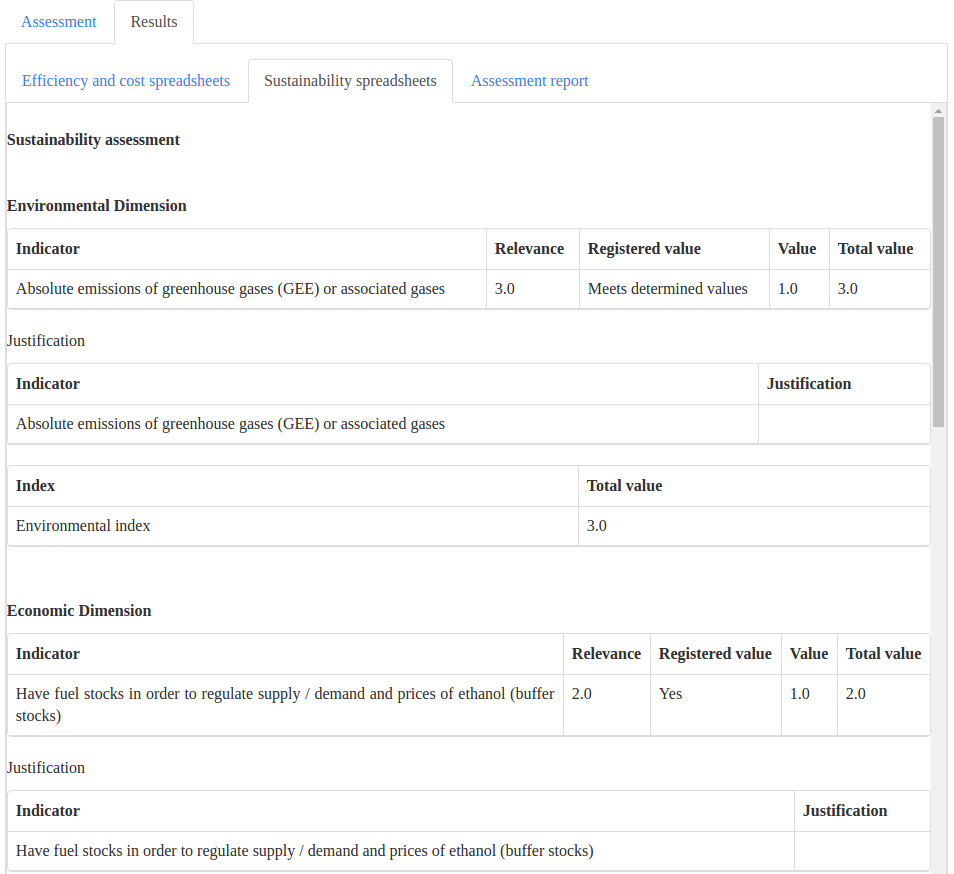
\includegraphics[width=1\columnwidth]{figures/SustenAgro-results}
\par\end{centering}
\caption{Planilhas do resultado da avaliação \label{fig:Planilhas-de-resultado}}
\end{figure}

\selectlanguage{english}%

\section{Web Components}

\selectlanguage{brazil}%
Foram desenvolvidos dois \foreignlanguage{english}{Web Components}
específicos para o SustenAgro. Eles geram gráficos específicos do
relatório solicitado pelos especialistas da Embrapa Meio Ambiente 

\subsection*{Matriz de Sustentabilidade}

Com a finalidade de suportar a geração de relatórios, no formato definido
pelos especialistas do domínio, foi necessário implementar dois \foreignlanguage{english}{Web
Component} especificos. Um deles foi a \foreignlanguage{english}{widget}
intitulada Matriz de Sustentabilidade. Ela é composta por dois eixos
que correspondem ao índice de eficiência, eixo Y, e ao índice de sustentabilidade,
eixo X. Os índices tem magnitudes que são dividas em segmentos que
permitem dividir a área em doze quadrantes da sustentabilidade. Cada
avaliação realizada com o método SustenAgro gerará dois índices que
são localizados em um quadrante da matriz de sustentabilidade. Cada
quadrante está relacionado com uma recomendação específica. A Figura
\ref{fig:Matriz-de-sustentabilidade} mostra a implementação desse
\foreignlanguage{english}{Web Component,} mostrando resultados reais
de uma avaliação.

\begin{figure}[H]
\noindent \begin{centering}
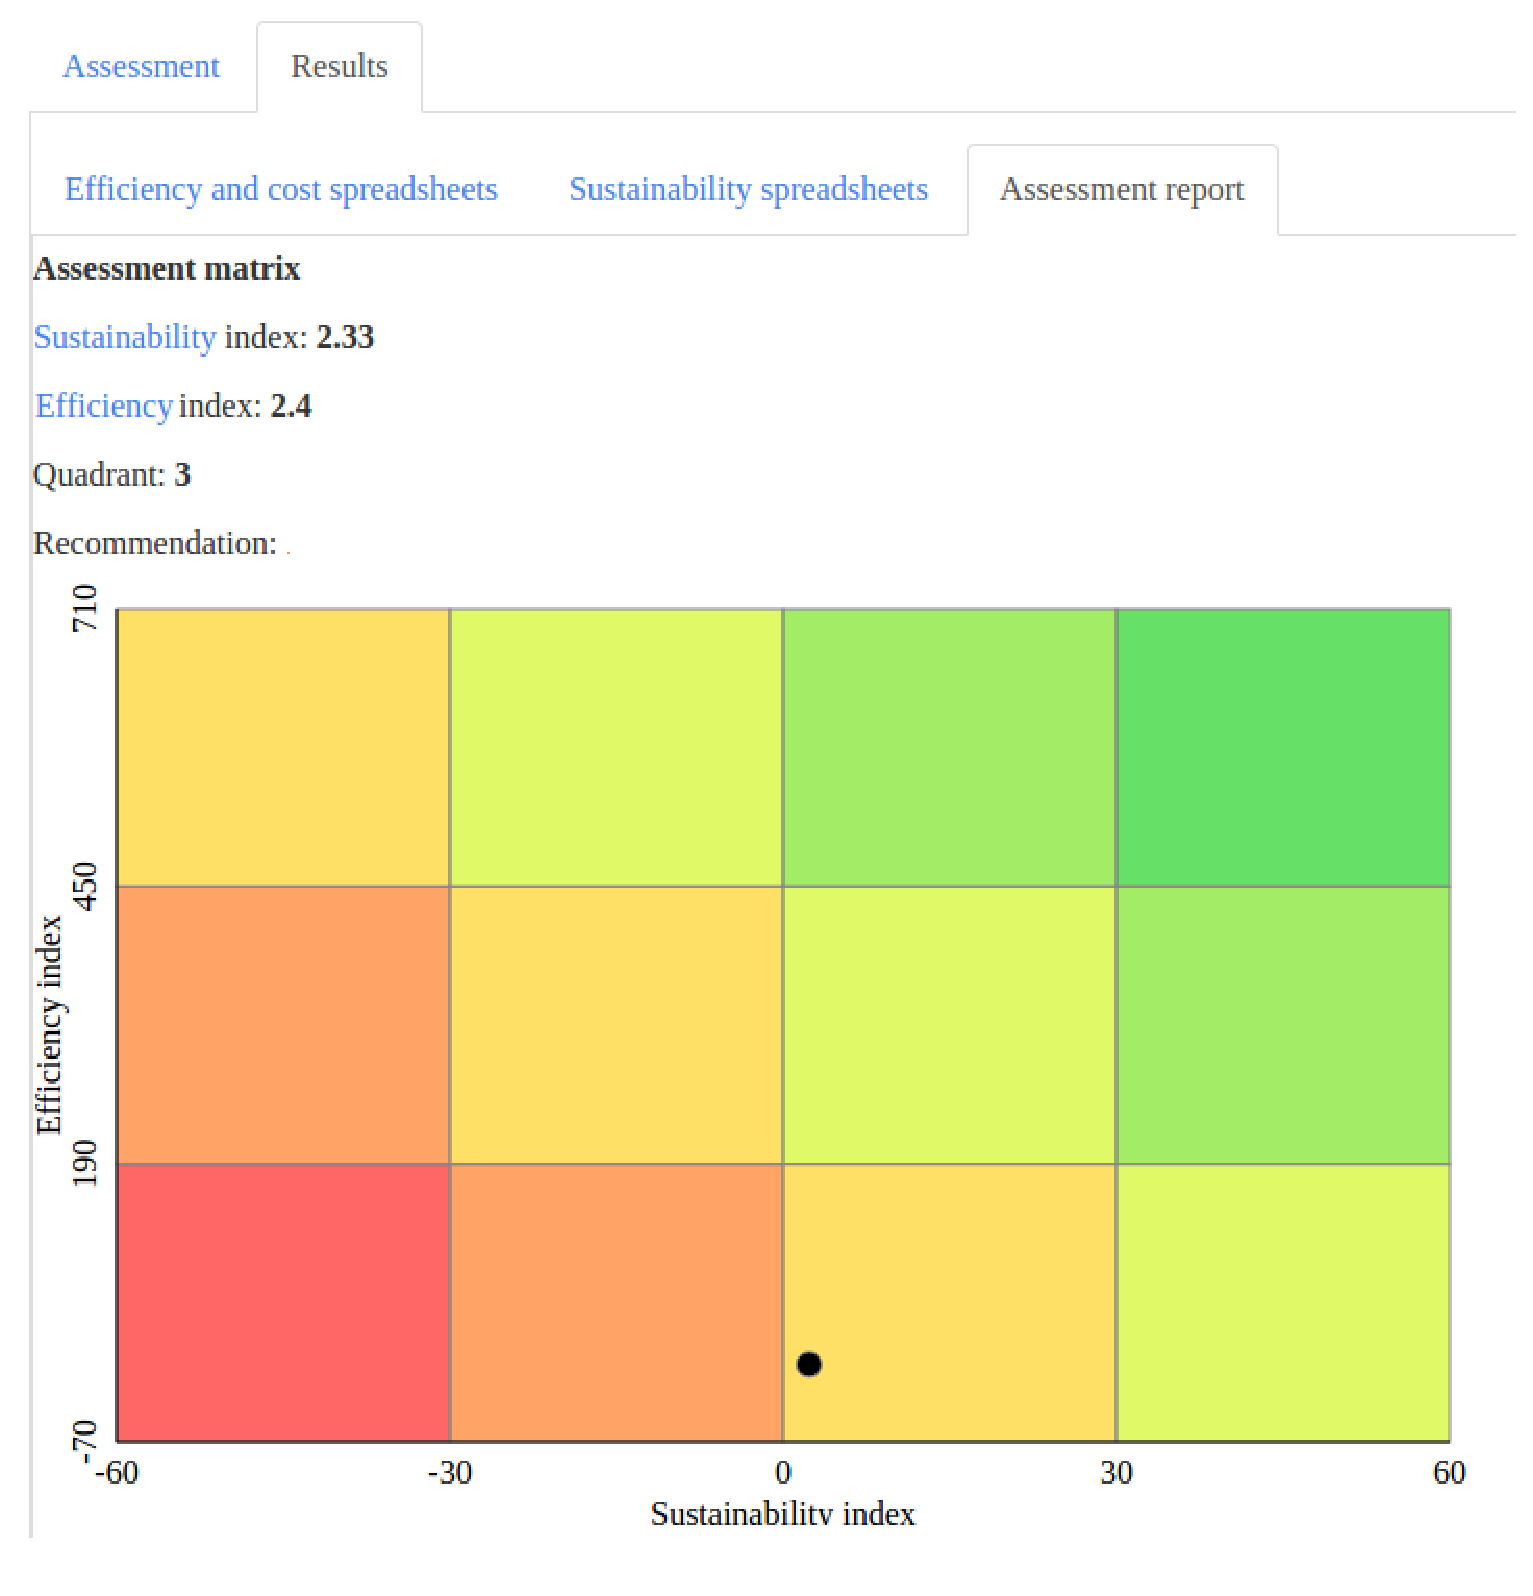
\includegraphics[width=1\columnwidth]{figures/SustenAgro-matrix}
\par\end{centering}
\caption{Matriz de sustentabilidade\label{fig:Matriz-de-sustentabilidade-widget}}
\end{figure}


\subsection*{Semáforo da Sustentabilidade}

O \foreignlanguage{english}{Web Component} do Semáforo da Sustentabilidade
foi o segundo componente para geração de relatórios, no formato definido
pelos especialistas do domínio, desenvolvido para o método SustenAgro.
Ele tem um eixo que quantifica o valor da sustentabilidade normalizado
entre -100 até +100, dividindo o intervalo em 5 segmentos que correspondem
às categorias de sustentabilidade. A Figura \ref{fig:Sem=0000E1foro-de-sustentabilidade}
mostra esse componente no sistema SustenAgro com os valores para uma
avaliação de sustentabilidade.

\begin{figure}[H]
\noindent \begin{centering}
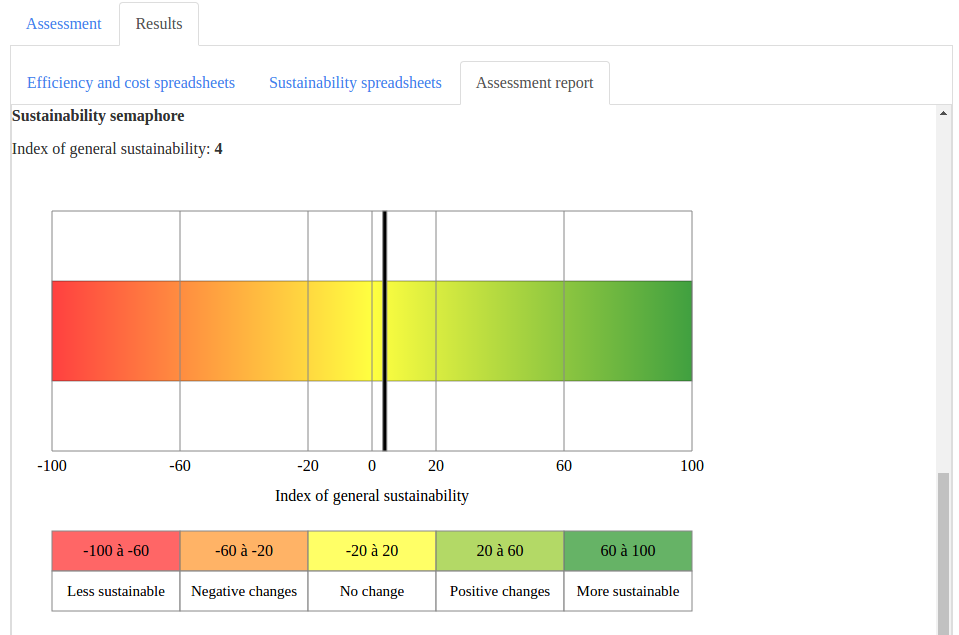
\includegraphics[width=1\columnwidth]{figures/SustenAgro-semaphore}
\par\end{centering}
\caption{Semáforo de sustentabilidade \label{fig:Sem=0000E1foro-de-sustentabilidade}}

\end{figure}

\selectlanguage{english}%

\section{DSL: code}

\selectlanguage{brazil}%
A implementação de uma DSL permite aos especialistas do domínio definir
como são usados e apresentados os conceitos da ontologia, por meio
de elementos da interface gráfica, como os índices de sustentabilidade
serão calculados e quais os elementos presentes no relatório final.
A DSL permite a criação de SADs facilmente adaptáveis às mudanças
do domínio. Os próprios especialistas podem modificá-la sem o auxílio
de programadores.

Para definir o comportamento do SustenAgro, especialistas tiveram
que:

\subsection{Definir o Objeto da Avaliação}

No comando, a seguir, o Objeto de Avaliação é definido como uma instância
da classe ProductionUnit. Essa classe foi definida pelos próprios
especialistas na ontologia e tem como filhos as classes . Também
são declaradas todas as propriedades que os usuários terão que preencher
quando criarem uma avaliação. Por exemplo, na propriedade \textit{hasName}
os usuários devem preencher o nome da unidade de produção.

\inputencoding{latin9}\begin{lstlisting}
evaluationObject ':ProductionUnit', {             
  instance 'ui:hasName', label: ['en': 'Production unit or farm name', 'pt': 'Nome da unidade produtiva ou fazenda'], placeholder: ['en': 'Name', 'pt': "Nome"]
  instance ':hasAgriculturalProductionSystem', label: ['en': 'Agricultural production system' , 'pt': "Sistema de produ��o agr�cola"], header: ['en': 'Options', 'pt': "Op��es"]     
  type label: ['en': "Production unit type", 'pt': "Tipo da unidade produtiva"], header: ['en': 'Options', 'pt': "Op��es"]
  instance  ':hasSugarcaneSource', label: ['en': 'Sugarcane source', 'pt': "Origem da cana"], header: ['en': 'Options', 'pt': "Op��es"], multipleSelection: true, required: true
  instance 'dbp:state', label: ['en': 'State', 'pt': 'Estado'], header: ['en': 'States', 'pt': 'Estados']
  instance 'ui:hasMicroregion', label: ['en': 'Production unit microregion', 'pt': "Microrregi�o da unidade produtiva"], header: ['en': "Options", 'pt': "Op��es"]
  instance ':hasAvailabilityOfEvaluationResults', label: ['en': "Availability of evaluation results", 'pt': "Disponibiliza��o dos resultados da avalia��o"], header: ['en': "Options", 'pt': "Op��es"]
}
\end{lstlisting}
\inputencoding{utf8}

\subsection{Definir as características a serem avaliadas}

Agora os especialistas têm que escolher quais características (Features)
dos Objetos de Avaliação serão usadas. No comando \textit{feature},
são indicadas as classes das \textit{Features} a serem usadas. Serão
mostradas todas as \textit{features} das classes indicadas e de suas
descendentes. Por exemplo, o comando \textit{feature ':ProductionEfficiencyFeature'}
vai mostrar todas as \textit{Features} relacionadas com eficiência
da produção. Na ontologia SustenAgro foram estabelecidas as famílias
de \foreignlanguage{english}{\textit{Features}}: EnvironmentalIndicator,
EconomicIndicator, SocialIndicator, ProductionEfficiencyFeature e
TechnologicalEfficiencyFeature.

O comando \textit{feature} também permite dizer se existirão novas
\textit{Features} criadas pelos usuários ('extraFeatures': true) e
a apresentação condicional de grupos de Features. No exemplo da Listagem
, são mostradas Features industriais apenas à usuários de usinas.

\inputencoding{latin9}\begin{lstlisting}
feature ':EnvironmentalIndicator', 'extraFeatures': true 
feature ':EconomicIndicator', 'extraFeatures': true 
feature ':SocialIndicator', 'extraFeatures': true 
feature ':ProductionEfficiencyFeature' 
feature ':TechnologicalEfficiencyFeature', {          
  conditional ":ProductionUnit", 'http://dbpedia.org/ontology/Provider', {
    include ':TechnologicalEfficiencyInTheField'          
  }
  conditional ":ProductionUnit", 'http://dbpedia.org/resource/PhysicalPlant', {
    include ':TechnologicalEfficiencyInTheField', ':TechnologicalEfficiencyInTheIndustrial'          
  }  
}
\end{lstlisting}
\inputencoding{utf8}

\subsection{Definir o modelamento e a forma de apresentação dos resultados}

Finalmente, no comando \textit{data}, os especialistas definem o nome
da variável que contém as respostas dos usuários e, no comando \textit{report},
fazem o cálculo do modelamento e definem o que vai ser apresentado.
Na listagem , é possível ver o cálculo dos índices de sustentabilidade
e eficiência através das formulas do modelo usado pelo SustenAgro.
É possível usar qualquer comando da linguagem Groovy ou biblioteca
externa. As variáveis guardam os valores de interesse que serão mostrados
no relatório de avaliação. No caso do SustenAgro, a variável \foreignlanguage{english}{\textit{sustainability}}
guarda o índice de sustentabilidade e a variável \textit{efficiency}
guarda o índice de eficiência do sistema.

No relatório aparecerão a Matriz de Sustentabilidade (SustainabilityMatrix),
o Semáforo de Sustentabilidade (SustainabilitySemaphore), o texto
\textquotedbl{}Mapa da Microregião\textquotedbl{} e o mapa da microregião
(onde a unidade produtiva se encontra). Cada uma dessas widget é instanciada
na DSL e os valores de interesse são passados para os Web Components
encarregados da apresentação. O framework Decisioner delega aos Web
Components a tarefa de apresentação.

Usuários podem pedir a geração de relatórios em pdf, uma ferramenta
de conversão de HTML para pdf é usada.

\inputencoding{latin9}\begin{lstlisting}[caption={SustenAgro DSL },label={lis:DSL-SustenAgro}]
data 'data'
report {       
  environment =   weightedSum(data.':EnvironmentalIndicator')

  economic    =   weightedSum(data.':EconomicIndicator')     
 
  social      =   weightedSum(data.':SocialIndicator')  

  sustainability = (environment + social + economic)/3

  cost_production_efficiency = sum(data.':ProductionEfficiencyFeature')

  technologicalEfficiencyInTheField = 0.8*weightedSum(data.':TechnologicalEfficiencyInTheField')

  technologicalEfficiencyInTheIndustrial = 0.2*weightedSum(data.':TechnologicalEfficiencyInTheIndustrial')

  efficiency = Math.abs(cost_production_efficiency) * (technologicalEfficiencyInTheField+technologicalEfficiencyInTheIndustrial)

  sustainabilityMatrix x: sustainability, y: efficiency,  
                       label_x: ['en': 'Sustainability Index', 'pt': '�ndice de Sustentabilidade'],                 
                       label_y: ['en': 'Efficiency index', 'pt': '�ndice de Efici�ncia'],
                       range_x: [-43,43],
                       range_y: [-160,800],
                       quadrants: [4,3]                       
   
  sustainabilitySemaphore value: sustainability,                  
                          label: ['en': 'Sustainability Level', 'pt': '�ndice da sustentabilidade geral'],
                          legend: [['en': 'Lower sustainability', 'pt': 'Menos sustent�vel'],
                                  ['en': 'Negative changes', 'pt': 'Altera��es negativas'],
                                  ['en': 'Irrelevant changes', 'pt': 'Sem altera��o'],
                                  ['en': 'Positive changes', 'pt': 'Altera��es positivas'],                                     
                                  ['en': 'Higher sustainability', 'pt': 'Mais sustent�vel']],
                          range: [-60,60]    

  text 'en': 'Microregion map', 'pt': '**Mapa da microregi�o**'    

  map data.'Microregion'   
}     
\end{lstlisting}
\inputencoding{utf8}

\section{Considerações Finais}

O desenvolvimento do sistema Sustenagro satisfez uma necessidade presente
na unidade da Embrapa Meio Ambiente: um sistema de avaliação de sustentabilidade
em cana-de-açúcar no centro-sul do Brasil. O SAD SustenAgro representa
e permite complementar informações e dados do estado atual de sustentabilidade
nas fazendas e usinas. Ele produz relatórios com a finalidade de embasar
e formalizar políticas para promover práticas produtivas mais sustentáveis,
de acordo com critérios ambientais, sociais e econômicos.

Além de satisfazer uma necessidade institucional, o SustenAgro é uma
proposta de SAD baseado em conhecimento e vinculado às tecnologias
da web semântica. O SustenAgro não foi apenas uma instanciação do
framework Decisioner, ele definiu o próprio framework. Através do
desenvolvimento do SustenAgro, foi possível determinar as características
gerais desse tipo de SAD, e implementá-las no framework, e as características
específicas do Sustenagro, que foram implementadas usando a ontologia
SustenAgro, os dois Web Components e a DSL.

Tendo o sistema SustenAgro instanciado e rodando, foi possível validar
suas funcionalidades através de alguns experimentos com integrantes
do projeto SustenAgro da Embrapa. Os resultados obtidos nas avaliações
dos experimentos serão detalhados no próximo capítulo.


\chapter{Avaliação\label{chap:Avalia=0000E7=0000E3o}}

O SAD SustenAgro (capítulo \ref{chap:SustenAgro}) foi instanciado
usando o Framework Decisioner (capítulo \ref{chap:Decisioner}) e
avaliado, durante diferentes estágios de desenvolvimento, através
de experimentos realizados com especialistas de domínio e usuários
da Embrapa. Esses dois sistemas foram desenvolvidos com metodologias
iterativas, onde foram realizadas varias inspeções e testes durante
a implementação. Uma avaliação final também foi realizada para analisar
se as funcionalidades foram implementadas corretamente.

A seguir, são apresentadas as avaliações realizadas no SAD SustenAgro
e ao Framework Decisioner. Elas foram independentes e geraram resultados
que levaram ao redesenho das arquiteturas de ambos sistemas em diferentes
etapas do seu desenvolvimento.

\section{Avaliação das Web UI.}

Na finalização do processo de design das Web UI, explicado na Seção
\ref{sec:Web-UI}, foi realizada uma avaliação da usabilidade das
mesmas no SAD SustenAgro. Os detalhes dessa avaliação foram:
\begin{description}
\item [{Data}] Junho de 2015
\item [{Participantes}] Usuários da ferramenta: especialista em sustentabilidade
e especialista em economia agrícola
\item [{Local}] Instituto de Ciências Matemáticas e de Computação (ICMC-USP)\nomenclature{ICMC}{ Instituto de Ciências Matemáticas e de Computação} 
\item [{Técnica}] Avaliação de usabilidade
\end{description}
Nesta avaliação foi apresentado, aos usuários especialistas em sustentabilidade,
o processo de design da UI e o protótipo da interface gráfica de usuário
do SAD SustenAgro sem dados reais. Nessas interfaces, eles interagiram
com as telas, através de um navegador web, fazendo uso das funcionalidades
do SAD que simulava os dados durante o processo.

Durante esta avaliação foram verificados, os três aspectos da usabilidade:
\begin{itemize}
\item Eficácia: as interfaces permitiram realizar as tarefas segundo as
funcionalidades definidas e permitiam interagir de maneira intuitiva
para realizar as tarefas.
\item Eficiência: o aceso à ferramenta foi realizado em tempos esperados
e foi possível realizar as tarefas com recursos típicos de um laptop
e um navegador web.
\item Satisfação: os usuários conseguiram realizar as tarefas sem problemas
e com uma experiência de fácil uso, onde a ferramenta fornecia informação
de ajuda para realizar as interações.
\end{itemize}
A avaliação foi positiva, cumprindo os três requisitos anteriores
de usabilidade. Esta avaliação gerou várias recomendações para melhorar
a interface gráfica de usuário, entre elas as mais relevantes foram: 
\begin{itemize}
\item Mudar a organização do processo de avaliação, agrupando varias tarefas
em uma seção denominada ``caracterização da unidade produtiva'',
que permite definir a localização, as principais características e
a disponibilização da informação em um processo unificado. 
\item Agrupar os resultados em uma seção ``Resultados'', integrando os
\foreignlanguage{english}{Web Components} específicos do SustenAgro
com os resultados da avaliação.
\item Organizar os indicadores em uma hierarquia simplificada que facilita
o preenchimento dos mesmos.
\end{itemize}
Depois de implementar as recomendações anteriores, foi continuado
o desenvolvimento com a integração da ontologia SustenAgro e da DSL.
Foi necessário realizar ajustes da interface ao integrar cada funcionalidade.
As principais mudanças foram realizadas devido a esta avaliação.

\section{Avaliação da ontologia de domínio de avaliação da sustentabilidade.}

A ontologia SustenAgro foi o resultado da modelagem do conhecimento
dos especialistas, que passou por várias etapas, desde ser definida
em texto, modelada em mapas conceituas e criada a ontologia em \foreignlanguage{english}{OWL}
(esse processo foi detalhado na Seção \ref{sec:Metodologia}). Cada
uma dessas etapas requereu inspeções por parte dos especialistas para
verificar a correta modelagem, uma avaliação formal foi realizada
e os detalhes são descritos a seguir.
\begin{description}
\item [{Data}] 14 de abril do 2016
\item [{Participantes}] Especialista em sustentabilidade e especialista
em modelagem de conhecimento
\item [{Local}] Embrapa Informática Agropecuária - Campinas
\item [{Técnica}] Visualização da ontologia e recuperação de conhecimento
\end{description}
O especialista em modelagem de conhecimento da Embrapa Informática
Agropecuária e o especialista em sustentabilidade reuniram-se para
realizar a revisão da ontologia SustenAgro por meio de ferramentas
de engenharia de conhecimento que permitiram visualizar as ontologias.

As ferramentas usadas na avaliação foram yWorks \footnote{\url{http://www.yworks.com/}}
e Gephi \footnote{\url{https://gephi.org/}}. Elas representaram aspectos
da ontologia usando diversas visualizações de grafos, permitindo avaliar
a coerência das conexões entre os nós daqueles grafos.

Também foi analisado o SAD SustenAgro, que tinha a ontologia integrada,
usando as funcionalidades que requeriam dados da ontologia, verificando
a informação recuperada e a coerência dela em relação à existente
na ontologia. 

A reunião de avaliação chegou no consenso: a ontologia \foreignlanguage{english}{OWL}
está representando a avaliação da sustentabilidade do sistema de produção
de cana no centro-sul do Brasil, destacando a especificidade dela
para suportar o SAD Sustenagro e que seu foco em conceitos concretos.

Foi recomendado integrar outros tipos de visualizações e editores
de ontologia no framework Decisioner. Entre eles foi recomendado fornecer
um editor visual de ontologias, basado na ferramenta \foreignlanguage{english}{WebVOWL,}
definida e desenvolvida por \citet{lohmann2014webvowl}. Devido a
limitações de tempo, não foi possível a implementação dessa sugestão
específica.

\section{Avaliação do protótipo funcional com dados}

Com a finalidade de avaliar a implementação do método SustenAgro,
foram realizados testes de vários tipos de avaliações, para comparar
com resultados de outras fontes, e assim validar a correta implementação.
Os detalhes da avaliação foram.
\begin{description}
\item [{Data}] 6 de junho do 2016
\item [{Participantes}] Especialista em sustentabilidade e especialista
em economia agrícola
\item [{Local}] Agência Paulista de Tecnologia dos Agronegócios (APTA)
\item [{Técnica}] Testes numéricos dos resultados do software
\end{description}
A revisão dos resultados numéricos foi realizada a partir de vários
cenários de indicadores, sendo realizada uma comparação dos resultados
processados manualmente com os resultados de avaliação do SAD SustenAgro.
Os resultados manuais foram iguais aos calculados pelo sistema, o
que permitiu validar a correta definição do método SustenAgro e sua
implementação no SAD SustenAgro. 

Os cenários avaliados foram casos extremos dos indicadores, processo
denominado teste de mínimos e máximos, gerando resultados em forma
de relatório para cada um dos cenários. 

A Figura \ref{fig:Matriz-de-sustentabilidade-Minimos} apresenta a
Matriz de Sustentabilidade com o cenário de mínimos, na qual o ponto
preto identifica o resultado da avaliação. Ele ficou no primeiro quadrante
tal como se esperava. Os resultados para testes de máximos também
se comportaram como esperado.

\begin{figure}[H]
\begin{centering}
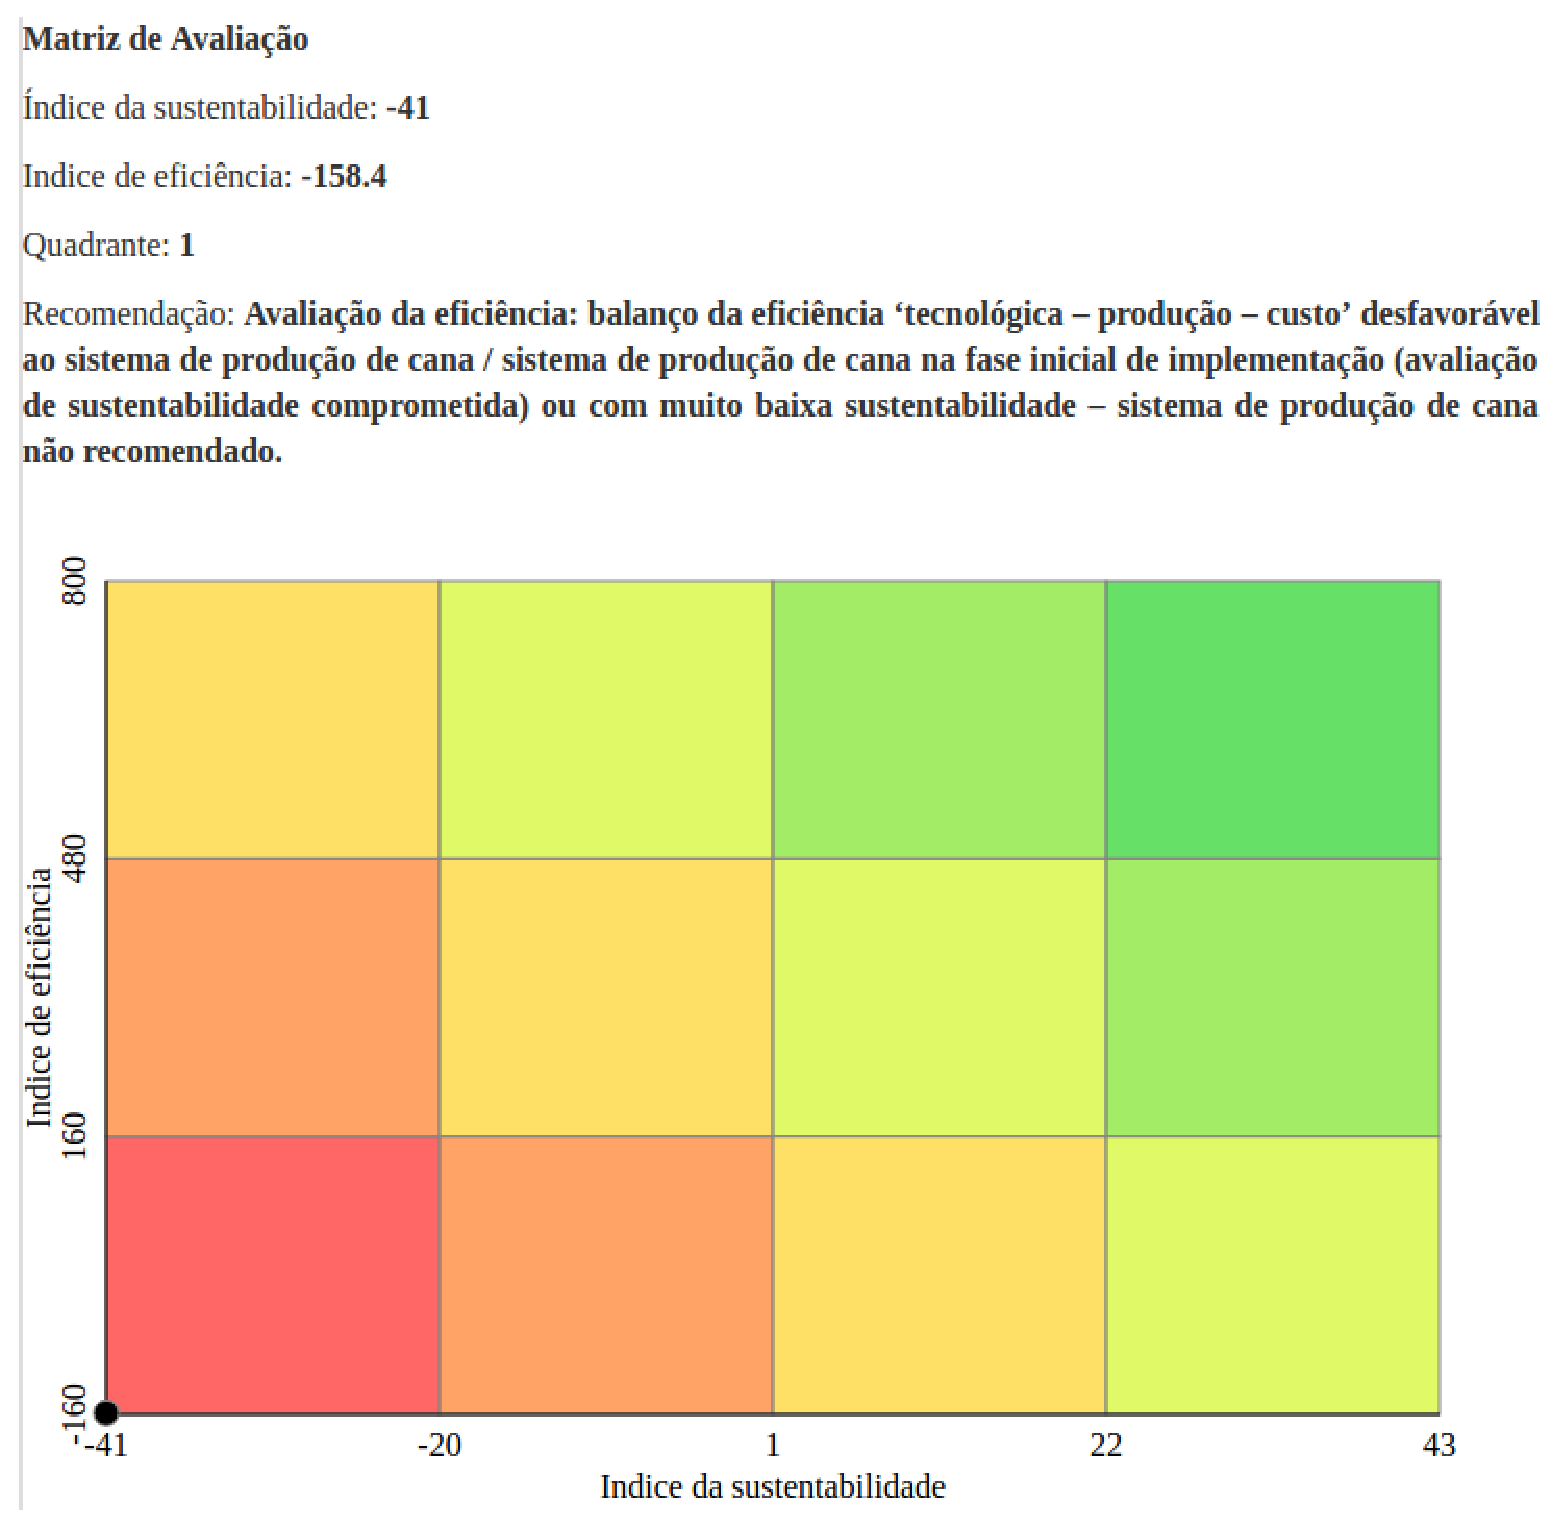
\includegraphics[width=1\columnwidth]{figures/Minimum}
\par\end{centering}
\caption{Matriz de Sustentabilidade com valores mínimos.\label{fig:Matriz-de-sustentabilidade-Minimos}}

\end{figure}

 Durante a realização dos testes foi descoberto um problema na formula
do método SustenAgro original, e a avaliação efetuada permitiu contribuir
na redefinição da formula de avaliação, por meio da integração de
uma operação de valor de um valor absoluto na fórmula. A possibilidade
da interação direta e fácil dos especialistas, em tempo real, com
o sistema permitiu demostrar agilmente possíveis cenários de resolução
do problema e aceitar rapidamente uma solução, proposta pelo autor.

\section{Avaliação do SAD SustenAgro e do Framework Decisioner: }

A partir da avaliação da ontologia, da implementação do método SustenAgro
e do desenvolvimento das Web UI realizou-se uma avaliação do SAD com
a finalidade de avaliar a integração desses componentes.
\begin{description}
\item [{Data}] 18 de maio do 2016 até o dia 22 de junho do 2016
\item [{Participantes}] Usuários especialistas e usuários finais.
\item [{Local}] Instituto de Ciências Matemáticas e de Computação (ICMC-USP)
\item [{Técnica}] Teste de usabilidade
\end{description}
Para realizar uma avaliação integral do SAD SustenAgro e do Framework
Decisioner, foi necessário fazer testes de usabilidade com usuários
de ambos os perfis do sistema (especialistas de domínio e usuários
finais). Essa avaliação foi realizada com a maioria dos membros da
equipe SustenAgro e com usuários finais, de maneira remota e independente,
totalizando 8 avaliações.

A avaliação consistiu em realizar um conjunto de tarefas com o SAD
SustenAgro v1.0 e responder se foi possível terminar a tarefa e as
sugestões. As tarefas e perguntas solicitadas aos usuários estão listadas
no Apêndice \ref{sec:Formul=0000E1rio-de-avalia=0000E7=0000E3o-SustenAgro}
e permitiram gerar os seguintes resultados das avaliações:

\begin{longtable}{|>{\centering}p{0.2\columnwidth}|>{\centering}p{0.2\columnwidth}|>{\centering}p{0.6\columnwidth}|}
\hline 
\textbf{\small{}Perfil de Usuário} & \textbf{\small{}Avaliação} & \textbf{\small{}Sugestões}\tabularnewline
\hline 
\hline 
{\small{}Usuário final 1} & {\small{}Positiva, realizou as 5 tarefas de usuário final com sucesso} & \begin{itemize}
\item {\small{}Aumentar a ajuda para cada funcionalidade}{\small \par}
\item {\small{}Barra de progresso durante a avaliação}{\small \par}
\item {\small{}Resultados de avaliação mais detalhados}
\end{itemize}
\tabularnewline
\hline 
\hline 
{\small{}Usuário final 2} & {\small{}Positiva, realizou as 5 tarefas de usuário final com sucesso} & \begin{itemize}
\item {\small{}Melhorar a explicação do processo de avaliação}{\small \par}
\item {\small{}Resultados numéricos com formatação }
\end{itemize}
\tabularnewline
\hline 
\hline 
{\small{}Usuário final 3} & {\small{}Positiva, realizou as 5 tarefas de usuário final com sucesso} & \begin{itemize}
\item {\small{}Segurança no cadastro da senha}{\small \par}
\item {\small{}Melhorar a localização do botão avaliar}{\small \par}
\item {\small{}Remover }\foreignlanguage{english}{{\small{}scroll}}{\small{}
externo}{\small \par}
\item {\small{}Salvar automaticamente os dados}
\end{itemize}
\tabularnewline
\hline 
\hline 
{\small{}Especialista em sustentabilidade} & {\small{}Positiva, realizou as 5 tarefas de usuário e as 5 tarefas
de especialista de domínio com sucesso} & \begin{itemize}
\item {\small{}Definir e acrescentar os termos de uso}{\small \par}
\item {\small{}Melhorar a sequencia de telas durante o cadastro de novo
usuário}{\small \par}
\item {\small{}Balão explicativo dos campos do formulário de nova unidade
produtiva, especificamente a propriedade de publicação dos dados}{\small \par}
\item {\small{}Definir o limite de caráteres para o campo de justificativa}{\small \par}
\item {\small{}Salvar avaliação ao mudar de aba}{\small \par}
\item {\small{}Justificativas sempre visíveis na tela de resultados.}{\small \par}
\item {\small{}Acrescentar bandeira em inglês e termos de uso}
\end{itemize}
\tabularnewline
\hline 
\hline 
{\small{}Especialista economia} & {\small{}Positiva, realizou as 5 tarefas de usuário e as 5 tarefas
de especialista de domínio com sucesso} & \begin{itemize}
\item {\small{}Salvar dados da seção automaticamente}{\small \par}
\item {\small{}Mudanças em alguns }\foreignlanguage{english}{{\small{}labels}}{\small \par}
\item {\small{}Mudanças nos indicadores}{\small \par}
\item {\small{}Componentes gráficos para representar os dados }{\small \par}
\item {\small{}Editor visual de ontologia e internacionalização}
\end{itemize}
\tabularnewline
\hline 
\hline 
{\small{}Especialista em ontologias} & {\small{}Positiva, realizou as 5 tarefas de usuário final com sucesso} & \begin{itemize}
\item {\small{}Melhorar a apresentação do botão salvar}{\small \par}
\item {\small{}Indicadores em forma de pergunta com verbo e simbolo de pergunta}{\small \par}
\item {\small{}Informar a possibilidade de edição de indicadores }
\end{itemize}
\tabularnewline
\hline 
\hline 
{\small{}Especialista agricultura} & {\small{}Positiva, realizou as 5 tarefas de usuário final com sucesso} & \begin{itemize}
\item {\small{}Cadastrar mais de uma microrregião}{\small \par}
\item {\small{}Remover }\foreignlanguage{english}{{\small{}scroll}}{\small{}
externo, mudanças em vários indicadores}{\small \par}
\item {\small{}Melhorar a localização do botão salvar e avaliar}{\small \par}
\item {\small{}Salvar a seção para não perder os dados}{\small \par}
\item {\small{}Melhorar a apresentação do pdf}
\end{itemize}
\tabularnewline
\hline 
\hline 
{\small{}Especialista em computação} & {\small{}Positiva, realizou as 5 tarefas de usuário final com sucesso} & \begin{itemize}
\item {\small{}Salvar a seção e os dados dela em tempo real}{\small \par}
\item {\small{}Integrar sistemas externos para poupar informação (caracterização
da unidade produtiva) }
\end{itemize}
\tabularnewline
\hline 
\end{longtable}

\begin{table}[H]
\caption{Avaliação do SAD SustenAgro}
\end{table}

A partir dessa avaliação integral, feita por usuários finais e administradores,
foram definidas várias melhorias a serem realizadas no Framework Decisioner
e o SAD SustenAgro. Devido às limitações de tempo e de desenvolvedores,
foram implementados apenas os ajustes visuais nas web UI, melhoras
na apresentação dos resultados, na geração do PDF e, principalmente,
a inclusão da linguagem inglês. Essa última mudança foi selecionada
como de especial importância, por parte dos especialistas. Neste documento,
são apresentadas várias telas, tanto em português como em inglês,
que foram geradas a partir da implementação dessa funcionalidade.
\selectlanguage{english}%

\section{Workshop\foreignlanguage{brazil}{: validação do software SustenAgro
v1.0 com equipe de especialistas.}}

\selectlanguage{brazil}%
A partir das melhoras realizadas na avaliação interna pelos dois tipos
de usuários do SAD SustenAgro, o sistema foi disponibilizado em servidos
web do ICMC. Esta publicação permitiu dar suporte a uma avaliação
no formato de \foreignlanguage{english}{workshop} com especialistas
de diversos perfis que tinham interesse no SAD SustenAgro. O \foreignlanguage{english}{Workshop}
foi intitulado ``Validação do software SustenAgro'', os detalhes
do \foreignlanguage{english}{workshop} são apresentados a seguir.
\begin{description}
\item [{Data}] 14 de julho do 2016
\item [{Participantes}] Equipe do projeto SustenAgro de várias unidades
da Embrapa
\item [{Local}] Embrapa Informática Agropecuária - Campinas
\item [{Técnica}] Delphi
\end{description}
O \foreignlanguage{english}{workshop} teve o objetivo de avaliar a
qualidade e acuidade do SAD SustenAgro em termos da clareza da informação
técnica apresentada nas interfaces, com vistas a garantir o entendimento
do usuário e possibilitar que a avaliação da sustentabilidade do sistema
de produção de cana-de-açúcar seja realizada da melhor forma possível. 

No \foreignlanguage{english}{workshop} foi apresentado o formulário
de avaliação (Seção \ref{sec:Formulario-Delphi-Workshop}) usando
a técnica \foreignlanguage{english}{Delphi} \citep{wright1985tecnica},
a um grupo de especialistas com perfis de varias áreas do conhecimento,
entre eles destacam-se:
\begin{itemize}
\item Especialista em sustentabilidade
\item Especialista em ciências agrícolas
\item Especialista em modelagem de conhecimento
\item Especialista em ciência e Tecnologia do Bioetanol
\item Especialista em ciências da computação
\item Especialista em economia agrícola
\item Especialista em biotecnologia
\item Mestrando em ciências da computação (sistemas web e multimídia)
\item Mestrando em Planejamento de Sistemas Energéticos
\end{itemize}
As interações com o sistema foram filmadas enquanto os usuários executavam
uma lista de tarefas. Monitores do ICMC ficavam estimulando os usuários
a falar o que estavam pensando (técnica Think Aloud \citep{davey1983think})
e os questionavam, quando tinham alguma dificuldade de interação.
Ao final, houve um \foreignlanguage{english}{debriefing} e foram também
colhidas mais sugestões de mudança. 

Os especialistas aprovaram a ferramenta tanto na interação como no
conteúdo dela, com as seguintes sugestões:
\begin{itemize}
\item As perguntas dos indicadores não são de fácil interpretação.
\item Colocar mais informações na interface para facilitar o uso dela, por
exemplo o significado de alinhamento dos indicadores.
\item Alguns indicadores estão repetidos.
\item Os resultados da avaliação deveriam estar por dimensão.
\item Demora para salvar os dados inseridos.
\item A informação dos site tem inconsistências em relação à informação
do pdf gerado.
\item A recomendações do relatório precisam mais detalhamento.
\end{itemize}
É interessante que muitas das sugestões não tem haver com aspectos
computacionais ou de interface, mas sim com o processo de avaliação
de sustentabilidade. Esse processo é de inteira responsabilidade dos
especialistas de domínio (e foge totalmente do escopo deste trabalho).
Isso foi um ponto positivo. É natural que especialistas em sustentabilidade
estejam muito mais interessados na sua área do que nos aspectos computacionais
do SAD SustenAgro. Uma boa interface é aquela que desaparece da mente
do usuário e permite que este se foque na sua tarefa. Neste caso,
a avaliação de sustentabilidade. Acreditamos que o SAD SustenAgro
atendeu bem a esse requisito.

\section{Avaliação de SAD SustenAgro nos servidores da Embrapa}

A partir da aprovação do SAD SustenAgro, por parte dos especialistas
no \foreignlanguage{english}{workshop}, foi autorizada a instalação
da ferramenta nos servidores da Embrapa Meio Ambiente. Essa instalação
foi um esforço coordenado entre o desenvolvedor do framework Decisioner
(o autor deste trabalho) e técnicos de informática da Embrapa.
\begin{description}
\item [{Data}] 18 de agosto do 2016
\item [{Participantes}] Especialista em Sustentabilidade e especialista
em TI
\item [{Local}] Embrapa Meio Ambiente - Campinas
\item [{Técnica}] Teste de integração
\end{description}
A instalação, coordenada pelo desenvolvedor do Framework Decisioner
e técnicos da Embrapa, foi problemática. A Embrapa não autoriza o
acesso físico ou via ssh aos servidor por parte de profissionais externos.
Por esta razão, foi criado um documento de instalação, descrito no
Apêndice \ref{chap:Instalation}. Nele estão as instruções para instalar
o Framework Decisioner e instanciar o SAD SustenAgro.

A instalação foi exitosa e o sistema está funcionando no endereço
\url{https://sustenagro.embrapa.br/}. Atualmente o endereço não está
no ar, pois o SAD SustenAgro está em processo de registro no Instituto
Nacional de Propriedade Intelectual (INPI), em nome da Embrapa e USP,
e a Embrapa ter uma política de exigir esse registro para liberação
para uso externo.

\section{Conclusões}

Essas avaliações permitiram verificar que os requisitos do Framework
Decisioner e do SAD SustenAgro foram implementados corretamente e
que atenderam as necessidades dos especialistas de domínio e usuários
finais, identificadas nos levantamentos de requisitos.

As avaliações ocorreram em diferentes fases do projeto e cada uma
trouxe correções e melhoras que foram implementadas, na medida do
possível, segundo a relevância de cada mudança e o tempo disponível
para desenvolvedor do projeto. Por ter sido desenvolvido em um processo
cíclico, cada iteração acrescentou novas funcionalidades que fizeram
mudar a arquitetura dos sistemas, gerando \foreignlanguage{english}{bugs}
e inconsistências. Na versão 1.0, os sistemas contam com funcionalidades
estáveis que permitem fornecer os serviços implementados. Correções
e sugestões recebidas durante a avaliação e não implementadas por
problema de tempo, foram deixadas como trabalhos futuros, que serão
apresentados no próximo capítulo juntamente com as conclusões.


\chapter{Conclusões\label{chap:Conclus=0000E3o}}

Os resultados obtidos são: 
\begin{enumerate}
\item Ontologia em formatos da web semântica (RDF/OWL) da avaliação da sustentabilidade
no sistema de cana-de-açúcar. 
\item Protótipo de ontologia de interfaces gráficas em formatos da web semântica
(RDF/OWL) 
\item Linguagem de domínio especifico DSL, Decisioner, para definir e permitir
administrar os parâmetros e processos do sistema SustenAgro 
\item Protótipo de sistema de geração de interfaces suportado nas tecnologias
da web semântica 
\item Formulários para recolha de dados sobre sustentabilidade em cana-de-açúcar,
e o processo de colheita dos dados de algumas usinas do estado de
São Paulo 
\item Protótipo do sistema web Sustenagro que integra as ontologias e a
DSL, fornecendo um comportamento configurável em tempo de execução
dos parâmetros, processos e das interfaces gráficas de usuário
\end{enumerate}
Uma das finalidades deste projeto é construir um gerador de sistemas
de apoio a decisão que consiga suportar outros domínios de conhecimento,
propondo para a comunidade uma metodologia de desenvolvimento e manutenção
que fique simples para os usuários finais e assim permitir que os
especialistas no domínio façam as mudanças sem precisas dos especialistas
de T.I.

\section{Trabalhos Futuros}

Este capítulo apresenta os resultados estão uma versão da ontologia
de domínio do SustenAgro e artefatos para o desenvolvimento da interface
visual do sistema: User Stories, Scenarios, Story Boards, Mockups
e um protótipo para a interface do SustenAgro.

Os resultados obtidos são: 
\begin{enumerate}
\item Ontologia em formatos da web semântica (RDF/OWL) da avaliação da sustentabilidade
no sistema de cana-de-açúcar. 
\item Protótipo de ontologia de interfaces gráficas em formatos da web semântica
(RDF/OWL) 
\item Linguagem de domínio especifico DSL, Decisioner, para definir e permitir
administrar os parâmetros e processos do sistema SustenAgro 
\item Protótipo de sistema de geração de interfaces suportado nas tecnologias
da web semântica 
\item Formulários para recolha de dados sobre sustentabilidade em cana-de-açúcar,
e o processo de colheita dos dados de algumas usinas do estado de
São Paulo 
\item Protótipo do sistema web Sustenagro que integra as ontologias e a
DSL, fornecendo um comportamento configurável em tempo de execução
dos parâmetros, processos e das interfaces gráficas de usuário
\end{enumerate}
Uma das finalidades deste projeto é construir um gerador de sistemas
de apoio a decisão que consiga suportar outros domínios de conhecimento,
propondo para a comunidade uma metodologia de desenvolvimento e manutenção
que fique simples para os usuários finais e assim permitir que os
especialistas no domínio façam as mudanças sem precisas dos especialistas
de T.I.


\bibliographystyle{abntex2-alf}
\bibliography{references/references}


\appendix

\chapter{Método SustenAgro de Avaliação de Sustentabilidade}

\label{chap:Sustainability_Assessment}Este anexo apresenta os principais conceitos relacionados com a avaliação
da sustentabilidade segundo segundo os fines do projeto SustenAgro,
e como foram usados no processo de avaliação de sustentabilidade.

\section{Sustentabilidade}

Não existe um consenso sobre a definição de sustentabilidade, mas
uma definição orientadora para os fins do presente projeto é a seguinte:
\begin{quotation}
``O desenvolvimento sustentável prevê o atendimento das necessidades
do presente sem comprometer a capacidade das gerações futuras de suprir
suas próprias necessidades, \foreignlanguage{english}{Brundtland Commission}''
\citet{Burton:1987,brundtland1987our}
\end{quotation}
Este conceito foi ratificado pela Conferência das Nações Unidas sobre
o Meio Ambiente e Desenvolvimento, a Rio-92 \citet{ehlers1996agricultura}
a Rio+20 \citet{ONU2012}, após do relatório \foreignlanguage{english}{Brundtland}
a ênfase do conceito desloca-se da integridade ambiental para o elemento
humano, gerando um equilíbrio entre as dimensões econômica, social
e ambiental \citet{van2005indicadores}.

\citet{gliessman2001agroecologia} teoriza que não há como encontrar
a sustentabilidade e, portanto, o seu conceito mais representativo,
pois a mesma permanece sempre no futuro, dado o compromisso que os
sistemas têm de garantir as necessidades das gerações futuras. Assim,
a sustentabilidade é algo relativo ao tempo, ou seja, um sistema pode
ser mais ou menos sustentável que outro dependendo do tempo em que
for avaliado e do entendimento da sustentabilidade neste contexto.

A sustentabilidade esta vinculada a vários domínios de conhecimento,
um deles é a sustentabilidade em agricultura, que é de especial interesse
na segurança alimentar. Em 2050 a população mundial atingirá 9.1 bilhões
de pessoas FAO (2013), o qual imporá enormes desafios para garantir
a sustentabilidade em meio do aumento de alimentos, por isso são necessários
incentivos e políticas para garantir a sustentabilidade em agricultura,
a través da geração de estratégias que permitam conhecer o estado
dos sistemas produtivos e melhorar segundo as necessidades identificadas.

Segundo \citet{van2008integrated} os sistemas agrícolas evoluem continuamente
e são afetados por uma gama de forças globais e locais, os aspectos
que mais influenciam na sustentabilidade da agricultura são os tecnológicos
e políticos, permitindo identificar e melhorar diversos aspectos da
produção agrícola. 

Uma estrategia para quantificar a sustentabilidade são a definição
métodos e metodologias de avaliação, as quais utilizam indicadores,
um exemplo deste enfoque é exposto por \citet{AlkanOlsson:2009} que
desenvolveu um \foreignlanguage{english}{\emph{framework}} de indicadores
que relaciona de uma maneira consistente as dimensões ambiental, econômica
e social do desenvolvimento sustentável, seu principal benefício é
uma relativa simplicidade na apresentação da informação e a possibilidade
de vincular os indicadores com objetivos políticos de cada dimensão
da sustentabilidade e assim facilitar a comparação dos impactos das
novas políticas em cada dimensão.

\section{Dimensões da Sustentabilidade}

As dimensões da sustentabilidade são classificações que permitem identificar
e agrupar conceitos de sustentabilidade\citep{AlkanOlsson:2009}.,
dependendo da teoria de sustentabilidade escolhida, existem diversas
propostas de dimensões que podem ser usadas segundo a finalidade da
pesquisa, um exemplo desta classificação é a assumida na pesquisa
de \citet{oliveira:2013} onde são definidas seis dimensões da sustentabilidade:
Ambiental, Social, Agrícola/Industrial, Produtos/Subprodutos, Tecnológica
e Política.

No caso do sistema SustenAgro determinou-se pela equipe de especialistas
em sustentabilidade fazer uma divisão segundo a proposta do Relatório
Brundtland \citep{brundtland1987our}, onde foram identificadas as
três dimensões da sustentabilidade: ambiental, social e econômica,
as quais têm a mesma importância gerando um equilíbrio.

Ditas dimensões são sistemas complexos que integram fenômenos de natureza
diversa \citep{simon1991architecture}, integrando três subsistemas:
(i) o subsistema ambiental que fornece as condições físicas, químicas
e biológicas que suportam o desenvolvimento das culturas, (ii) o subsistema
social que integra organizações e pessoas que realizam a produção,
relacionando-se internamente e externamente com os sistemas produtivos
e (iii) o subsistema econômico que estabelece as condiciones de oferta
e demanda dos produtos e subprodutos do sistema de produção agrícola;
das interações entre estes subsistemas, emerge um comportamento complexo
que requer uma abordagem holística e inter-relacionada para suportar
a tomada de decisões que garantam a sustentabilidade do sistema em
analise.

A Figura \ref{fig:sustainability_spheres} representa as três dimensões
com a sustentabilidade como a interseção entre elas.

\begin{figure}[h]
\begin{centering}
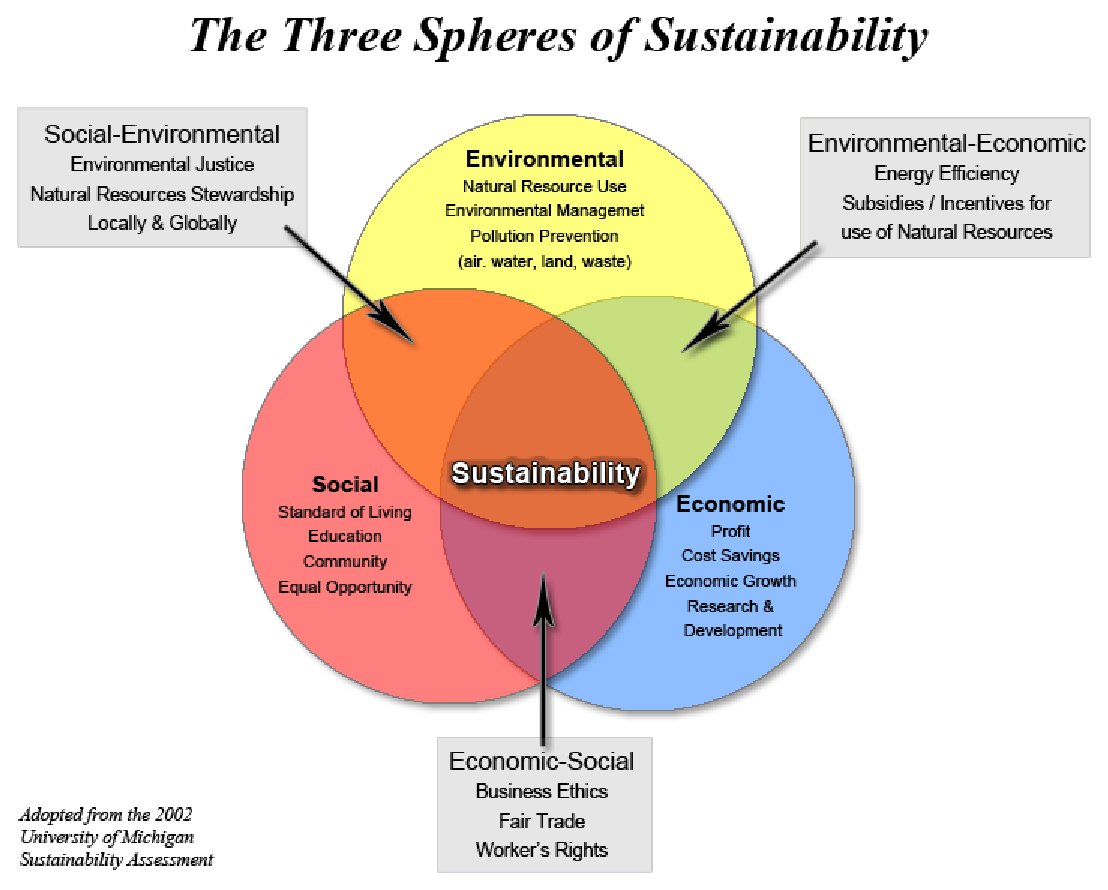
\includegraphics[width=1\columnwidth]{figures/sustainability_spheres}
\par\end{centering}
\caption{Dimensões da sustentabilidade \label{fig:sustainability_spheres}}
\end{figure}

\footnote{Tomada de: http://www.vanderbilt.edu/sustainvu/cms/files/sustainability\_spheres.png}Essas
dimensões serão usadas como contendedores gerais dos conceitos de
sustentabilidade em agricultura permitindo agrupar conceitos relacionados.

\section{Critérios de sustentabilidade}

São variáveis transversais quantitativas e qualitativas, que são monitoradas
regularmente para determinar os efeitos das atividades de intervenção
ou não-intervenção do sistema em avaliação \citet{deusdara2001criterios},
que estabelecem os preceitos de orientação para que os indicadores
sejam representativos para a sustentabilidade.

Cada indicador deverá atender pelo menos um dos critérios de sustentabilidade
para ser considerado um bom indicador de sustentabilidade, os critérios
de sustentabilidade escolhidos pela equipe de especialistas são\citet{moura2002indicadores}:
\begin{itemize}
\item Produtividade: Relacionado a eficiência e custos.
\item Estabilidade: Capacidade do ecossistema de absorver perturbações e
permanecer inalterado (Comissão Econômica para a América Latina e
o Caribe/Programa das Nações Unidas para o Meio Ambiente, CEPAL\nomenclature{CEPAL}{Economic Commission for Latin America and the Caribbean}/PNUMA\nomenclature{PNUMA}{Programa das Nações Unidas para o Meio Ambiente},
1994) 
\item Equidade: Distribuição dos produtos do agroecossistema entre produtores
e consumidores (Dias Junior, 2000) 
\item Resiliência: Capacidade do ecossistema de retornar ao estado original
após de uma perturbação (CEPAL/PNUMA, 1994) 
\item Autonomia: Grau de integração do agroecossistema no fluxo de materiais,
energia e informação entre as partes constituintes e entre o agroecossistema
e o ambiente externo (Fernández, 1995)
\end{itemize}
Esses critérios guiam o desenvolvimento dos conceitos mais relevantes
das metodologias de avaliação de sustentabilidade, os indicadores,
e assim determinar instrumentos de medição que representem os aspectos
críticos do sistema em termos de sustentabilidade.

\section{Atributos Norteadores}

Embora a orientação para a elaboração de todas as variáveis relacionadas
a projetos de sustentabilidade devam atender pelo menos a três pilares:
ambiental, econômico, social, os atributos norteadores são formulados
para garantir as diretrizes no levantamento e validação dos indicadores,
e assim ter um modelo da sustentabilidade dos sistemas de produção
agrícola.

Após a agregação dos dados será possível visualizar as informações
disponíveis e eventuais lacunas para a sistematização dos componentes
dos sistemas produtivos em termos dos requisitos de sustentabilidade.
Em uma primeira instância, devem ser levantados dados referentes ao
solo, clima, água, ar, produção agroindustrial, divisas geradas, mão
de obra envolvida, empregos gerados, doações/benefícios indiretos
à sociedade, biodiversidade, etc.

Uma proposta dos atributos norteadores é a seguinte:
\begin{itemize}
\item Dimensão Ambiental: solo, hídrico, clima, entre outros
\item Dimensão Social: saúde, capacitação, emprego, renda, entre outros
\item Dimensão Econômica: industrial, agrícola, produtividade, custo, entre
outros
\end{itemize}
Os atributos norteadores foram aplicados nos modelos do sistema SustenAgro
como contentores de indicadores os quais classificaram e relacionam
os indicadores em subgrupos das três dimensões da sustentabilidade,
permitindo desta maneira a organização e agrupamento do conhecimento
do domínio.

\section{Método SustenAgro}

Devido à importância da sustentabilidade, especialmente nos sistemas
de produção agrícola, foram desenvolvidas varias métodos para avaliar
o estado desses sistemas, existindo varias tendências segundo o tipo
de sistema produtivo e o contexto deles.

A Embrapa Meio Ambiente coordenou e financiou o projeto SustenAgro
com a finalidade de definir um método de avaliação da sustentabilidade
no sistema produtivo de cana-de-açúcar no centro sul do Brasil, as
características dele são descritas nas figuras \ref{fig:SustenAgro_Description}
e \ref{fig:SustenAgro_Details}, no qual foram originados os indicadores
de sustentabilidade e o método de avaliação \citep{oliveira:2013,BRUMATTI:2015}.

\vfill{}

\pagebreak{}

\begin{figure}[H]
\begin{centering}
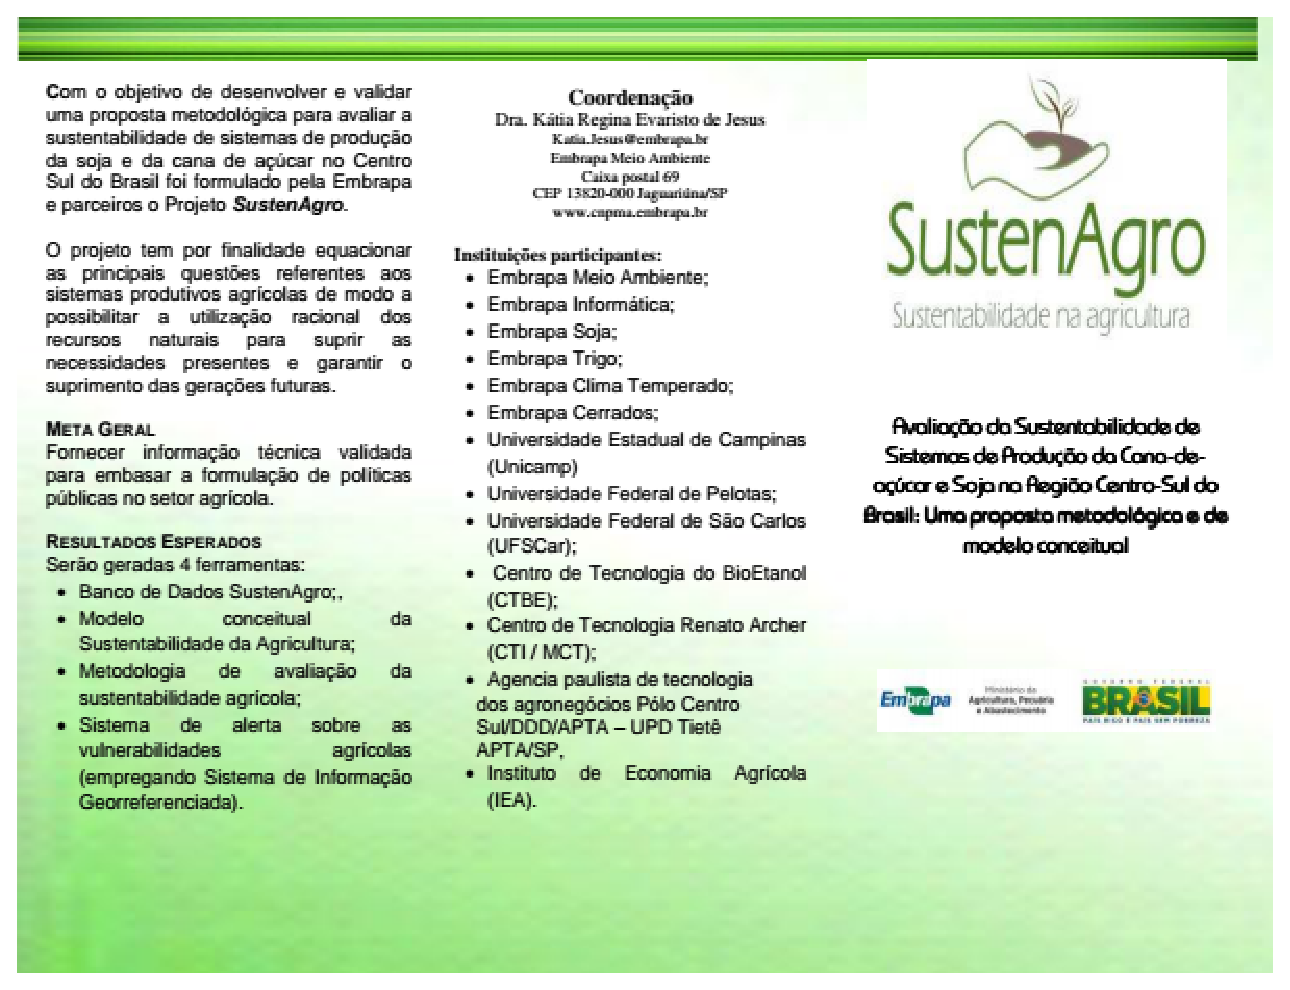
\includegraphics[width=1\columnwidth]{figures/folderEmbrapa1}
\par\end{centering}
\caption{Descrição geral do projeto SustenAgro \label{fig:SustenAgro_Description}}
\end{figure}

\begin{figure}[H]
\begin{centering}
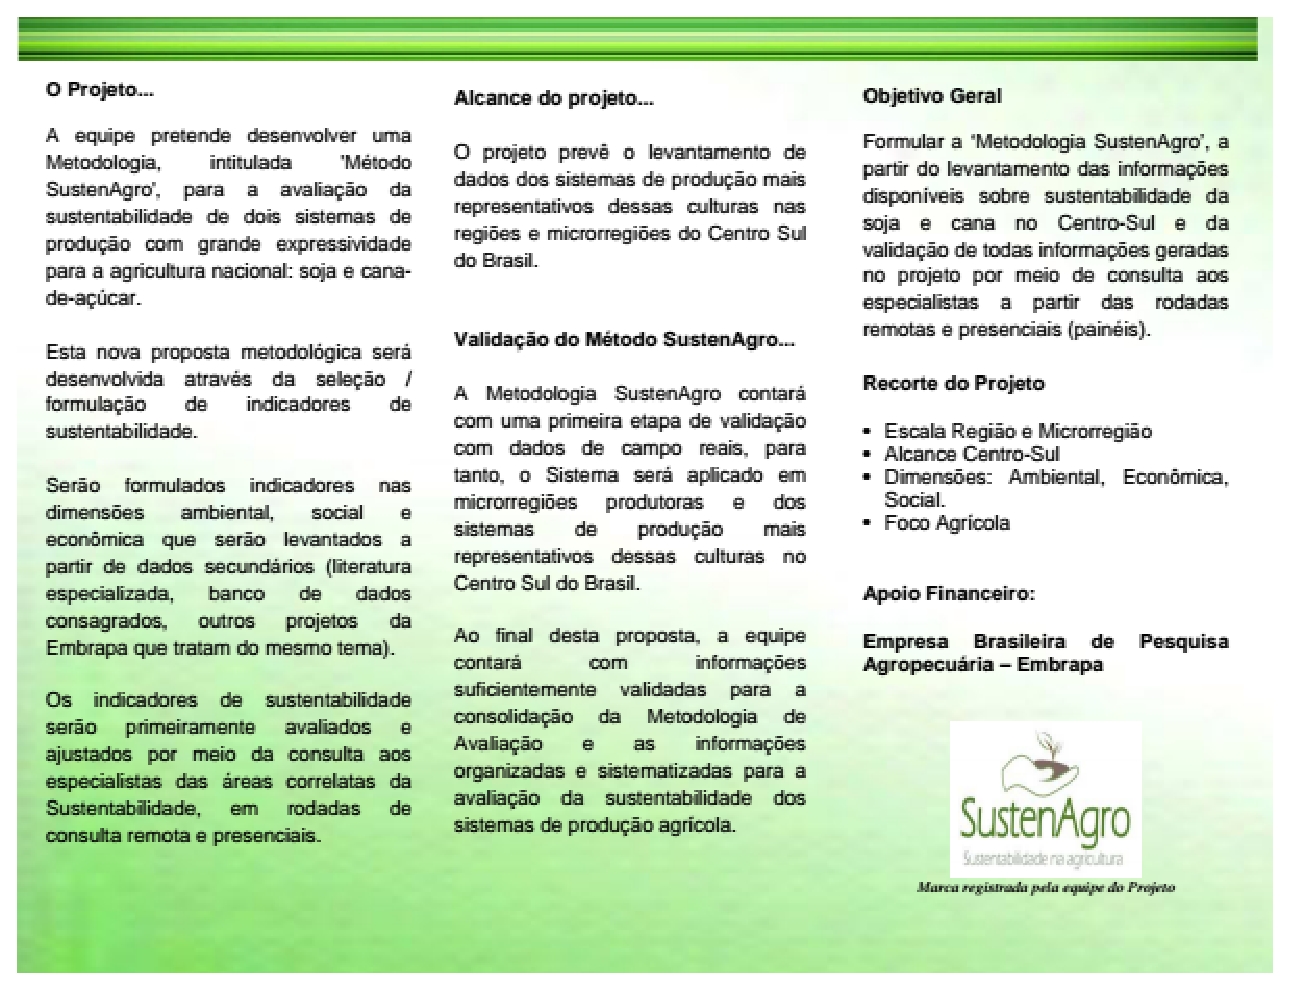
\includegraphics[width=1\columnwidth]{figures/folderEmbrapa2}
\par\end{centering}
\caption{Descrição especifica do projeto SustenAgro \label{fig:SustenAgro_Details}}
\end{figure}

O método SustenAgro foi construído a partir de literatura cientifica
e de instituições de pesquisa como (IBGE\footnote{IBGE: \foreignlanguage{english}{Brazilian Institute of Geography and
Statistics}, \url{http://www.ibge.gov.br/home/}}, CONAB \footnote{CONAB: \foreignlanguage{english}{National Supply Company}, \url{http://www.conab.gov.br/}})
e validados por meio da técnica \foreignlanguage{english}{Delphi}
de consultas aos especialistas.

O método esta composto de dos índices da eficiência e índice da sustentabilidade,
o índice da eficiência esta composto por dois fatores de eficiência
tecnológica no campo e na industria e o índice da sustentabilidade
está composto pelas dimensões ambientais, econômica e social.

\subsection*{Índice de eficiência:}

As equações para calcular o índice da eficiência são:

Formula de eficiência tecnologia no campo:

$efficiency(field)=\sum(CharacteristicsInTheField*RelevanceForTheProductionEnvironment)*correctionFactor(0.8)$

Formula de eficiência tecnologia na industria:

$efficiency(industry)=\sum(CharacteristicsOfProcessing*SugarcaneProcessingOptimization)*correctionFactor(0.2)$

Formula de eficiência produtiva e de costo:

$efficiencyAndCost=\sum(SugarcanEquality+\sum(Logistic+MarketVariables+Policies+Productivity))$

Índice de eficiência:

$EfficiencyIndex=\sum(efficiency(filed)+efficiency(industry))*efficiencyAndCost$

\subsection*{Índice de sustentabilidade}

As equações para calcular o índice de sustentabilidade são:

Formula de eficiência tecnologia no campo:

$EnvironmentalIndex=\sum(EnvironmentalIndicator*EnvironmentIndicatorWeight)$

Formula de eficiência tecnologia na industria:

$EconomicIndex=\sum(EconomicIndicator*EconomicIndicatorWeight)$

Formula de eficiência produtiva e de costo:

$SocialIndex=\sum(SocialIndicator*SocialIndicatorWeight)$

Índice de eficiência:

$SustainabilityIndex=\sum(EnvironmentalIndex+EconomicIndex+SocialIndex)/3$

\section{Matriz de sustentabilidade}

Os índices de eficiência e de sustentabilidade quantificam a sustentabilidade
de uma unidade produtiva, e são representados por meio de uma matriz
que tem como finalidade relacionar o resultado da avaliação com determinadas
classificações correspondentes a cada uns dos quadrantes da matriz,
a figura \ref{fig:Matriz-de-sustentabilidade} representa cada uma
das classificações com os limiares correspondentes a cada índice.

\begin{figure}[h]
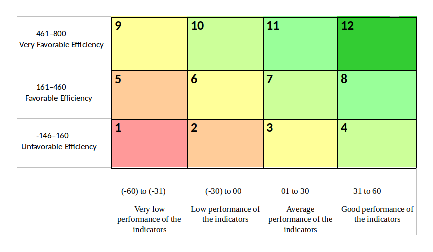
\includegraphics[width=0.8\columnwidth]{figures/SustaiabilityMatrixDesign}

\caption{Matriz de sustentabilidade \label{fig:Matriz-de-sustentabilidade}}

\end{figure}


\section{Conclusões}

O método de avaliação de sustentabilidade foi validado pelos especialistas
e depois de varias iterações definiu-se uma versão estável, que foi
usada no desenvolvimento do Sistema SustenAgro, dito método é mantido
e atualizado pela Embrapa Meio Ambiente e os desenvolvedores de software
garantem que ele se aplique corretamente mas não tem responsabilidade
nenhuma pelas consequências do uso dele.


\chapter{Indicadores de Sustentabilidade}

\label{chap:SustainabilityIndicators}
\section{Índice de Sustentabilidade}

O índice de sustentabilidade revela o estado de um sistema ou fenômeno,
sendo uma síntese das características ou variáveis analisadas. Um
índice pode ser construído para analisar dados através da junção de
um jogo de elementos com relacionamentos estabelecidos. Entende-se
o termo índice como um valor numérico que representa a correta interpretação
da realidade de um sistema simples ou complexo (natural, econômico
ou social), utilizando, em seu cálculo, bases científicas e métodos
adequados. O índice pode servir como um instrumento de tomada de decisão
e previsão \citep{SicheAgostinho2007}

No projeto SustenAgro os índices serão dados numéricos gerais representaram
a soma do estado de cada indicador em cada dimensão e atributo norteador.
Cada indicador pode o valor de mais um ou menos um (+1 -1), que permitirá
quantificar a sustentabilidade em cada aspecto do sistema produtivo
e fazer comparações com outros sistemas produtivos compatíveis.

\section{Limiares de Sustentabilidade}

Os limiares são os pontos mínimo e máximo aceitáveis na amplitude
da sustentabilidade para cada indicador.

Considerando que a sustentabilidade permanece sempre no futuro \citep{gliessman2001agroecologia},
dado o compromisso que os sistemas têm de garantir as necessidades
das gerações futuras, a sustentabilidade será considerada como algo
relativo no espaço e no tempo, ou seja, um sistema pode ser mais ou
menos sustentável do que outro.

Esta representação será realizada pelos limiares de sustentabilidade
que poderão variar de acordo com o sistema de produção considerado
e, principalmente, deve variar de modo a representar com propriedade
das especificidades regionais e microrregionais.

Dentro de uma escala, devem ser estabelecidos limiares críticos, ou
seja, aqueles em que concordamos que determinada situação (característica,
produto, serviço) apesar de não ser totalmente sustentável possui
níveis de sustentabilidade aceitáveis para que a sustentabilidade
seja efetiva (verdadeira), apesar de não ser a ideal. O limiar é um
ponto que estabelece um limite, geralmente é o princípio, mas no nosso
caso, são os limites que apontam que determinada característica, produto,
ou serviço, está dentro do que for considerado sustentabilidade, serão
os pontos mínimo e máximo aceitáveis na amplitude da sustentabilidade.

Dentro desta escala, estabelecemos limiares críticos, ou seja, aqueles
em que concordamos que determinada situação (característica, produto,
serviço) apesar de não ser totalmente sustentável (nota máxima), possui
níveis de sustentabilidade aceitáveis para que a sustentabilidade
seja efetiva (verdadeira), apesar de não ser a ideal. Neste caso,
o limiar mínimo de sustentabilidade assumiria um valor variável.

Exemplo de limiar da sustentabilidade que poderá ser empregada pela
equipe do projeto:
\begin{itemize}
\item Nome do Indicador: Distância Usina / Área de Produção de cana
\item Descrição do indicador: usualmente, em tradicionais regiões produtoras
de cana, utiliza-se de uma distância econômica padrão da produção
de 50 quilômetros até a indústria. Esta distância é determinada pelos
altos custos de transporte da cana até a unidade industrial, sendo
um dos fatores decisivos na rentabilidade da lavoura (CNA/SENAR, 2007).
\item Limiares de sustentabilidade, teria dois estados possíveis 

\begin{itemize}
\item Distância de até 50 km: Mais sustentável (+1)
\item Distância de mais de 50 km: Menos sustentável (-1)
\end{itemize}
\end{itemize}
Baseando-se no conceito de limiares é possível desenhar metodologias
de avaliação onde sejam usados os valores numéricos de cada limiar
para fazer comparações, o que permite definir se determinado sistema
produtivo e/ou contexto é mais sustentável do que outro sistema produtivo
e/ou contexto.

\section{Indicadores de Sustentabilidade}

Os indicadores são instrumentos usados para avaliar uma determinada
realidade levando em conta variáveis pertinentes para sua composição.
Além da avaliação, o uso de indicadores permite medir e monitorar
aspectos da realidade. Ele agrega, quantifica e simplifica informações
sobre fenômenos complexos de modo que as tendências ficam mais significativas
e aparentes, a fim de melhorar o processo de entendimento e comunicação\citep{bossel1999indicators,van2005indicadores}.

De acordo com \citet{gallopin1996environmental} os melhores indicadores
são aqueles que simplificam as informações relevantes, tornando os
fenômenos mais claros. Como um indicador é utilizado para atingir
diversos objetivos, é necessário definir um requisito geral para selecionar
indicadores e validar a escolha. A finalidade de um indicador de sustentabilidade
é refletir as alterações nas propriedades fundamentais de um sistema
\citep{CaminoAndMuller1993} e advertir sobre eventuais perturbações
potenciais\citep{ferraz2003}.

Normalmente um indicador é utilizado como um pré-tratamento aos dados
originais \citep{SicheAgostinho2007}. Indicadores são parâmetros
que podem ser utilizados como medida do cumprimento dos critérios
\citep{moret2006criterios}. Deve-se observar que não é possível o
desenvolvimento de um indicador global, por isso é necessário buscar
no tempo a evolução da sustentabilidade dos sistemas \citep{CaminoAndMuller1993}.
Não há indicadores universais, pois eles podem variar segundo o problema
ou objetivo da análise.

Quanto às características desejáveis para um bom indicador, deve-se
ter uma boa definição da fonte dos dados base para o levantamento,
possibilidade de calibração, possibilidade de comparação com critérios
legais ou outros padrões/metas existentes, facilidade e rapidez de
determinação e interpretação, grau de importância e validação científica,
sensibilidade do público-alvo, custo de implementação e possibilidade
de ser rapidamente atualizado. Nessa mesma linha, \citet{zampieri2003metodo}
baseado em vários autores, cita como requisitos para a seleção de
indicadores de avaliação de sustentabilidade: \renewcommand{\labelenumi}{\roman{enumi}.}
\begin{enumerate}
\item Serem mensuráveis quantitativa e qualitativamente, além de terem pertinência
ao objeto e à natureza do processo avaliado; 
\item Poder coletar as informações com baixo custo, ser de fácil execução
e apresentar dados cientificamente válidos; 
\item Serem concebidos para que o agricultor participe das medições, adaptados
às necessidades dos usuários da informação e estarem embasados em
linguagem clara; 
\item Serem sensíveis às mudanças do sistema ao detectar a magnitude dos
desvios e tendências, oferecendo prognósticos e perspectivas para
planejar e tomar decisões; 
\item Fornecerem indicação clara a respeito da sustentabilidade do sistema
estudado e refletirem os impactos estudados sob o enfoque integrado; 
\item Representarem padrões ecológicos, sociais, econômicos e espaciais,
que tenham correspondência e sensibilidade com o nível de agregação
do sistema considerado; 
\item Conter um nível de agregação que permita comparações individuais,
intertemporais e o cruzamento com outros indicadores; 
\item Fornecerem informações para avaliar os trade-offs entre as dimensões
da sustentabilidade e correlações com os processos dos ecossistemas; 
\item Poder ter repetibilidade, de modo que as medições possam ser realizadas
por diferentes pessoas e que os resultados sejam comparáveis
\item A construção do indicador deve observar parâmetros politicamente corretos.
\end{enumerate}
A OECD\footnote{Organisation for Economic Co-operation and Development \url{http://www.oecd.org/brazil/}}
estabelece três requisitos para selecionar indicadores: relevância
política e utilidade para usuários, solidez analítica e mensurabilidade. 

Alguns exemplos de indicadores levantados no desenvolvimento do método
SustenAgro são: 
\begin{enumerate}
\item Risco climático; 
\item Diversidade de culturas anuais; 
\item Tipo de solo; 
\item Risco de deficit hídrico; 
\item Produtividade da terra; 
\item Renovabilidade energética nos sistemas de produção; 
\item Balanço de nutrientes (nitrogênio e fósforo); 
\item Área de cultivo/áreas preservadas.
\end{enumerate}
Os indicadores do presente projeto são uma representação dos fatores
críticos que existem no sistema de produção de cana-de-açúcar no centro-sul
do Brasil em cada dimensão da sustentabilidade, pelo qual a metodologia
e o sistema SustenAgro é aplicável nesse contexto. No caso de quer
aplicar o sistema de avaliação da sustentabilidade em outro contexto
é necessário mudar os indicadores a cada contexto especifico. 

\section{Dados fornecidos pela Unidade de Meio Ambiente da Embrapa }

A principal fonte de dados para este projeto foi fornecida pela pesquisa
de \citet{oliveira:2013}, onde inicialmente foram identificados 62
indicadores de sustentabilidade no sistema de cana-de-açúcar, os quais
foram analisados e caracterizados, gerando 39 indicadores como os
mais relevantes \citep{BRUMATTI:2015}, por meio de uma validação
com porcentagem maior ou igual a 60\% feita por uma comunidade de
especialistas em sustentabilidade.

As seguintes tabelas mostram os indicadores resultantes, os quais
foram classificados nas três dimensões da sustentabilidade.

Os indicadores da tabela \ref{tab:Indicadores-de-sustentabilidade-ambiental}
representam os valores críticos da dimensão ambiental integrando fenômenos
do solo, dos recursos hídricos e climáticos, os quais permitem caracterizar,
quantificar e comparar o estado da dimensão ambiental de uma unidade
produtiva com outras.

\begin{table}[h]
\begin{tabular}{|>{\raggedright}p{14cm}|}
\hline 
\textbf{Indicadores da dimensão ambiental}\tabularnewline
\hline 
\hline 
Quantificação da erosão potencial segundo a Equação Universal de Perda
de Solo (USLE – \foreignlanguage{english}{Universal Soil Loss Equation})\tabularnewline
\hline 
Compactação do solo\tabularnewline
\hline 
Ocorrência de queimada de palha no campo\tabularnewline
\hline 
Emissão e suspensão de micropartículas (fuligem)\tabularnewline
\hline 
Localização geográfica da cultura em relação à aptidão agroclimática\tabularnewline
\hline 
Localização geográfica da cultura em relação à aptidão edáfica\tabularnewline
\hline 
Localização geográfica da cultura em relação à aptidão edafoclimática\tabularnewline
\hline 
Áreas de Preservação Permanente (APP) recuperadas/conservadas\tabularnewline
\hline 
Comprovação de averbação da área de Reserva Legal\tabularnewline
\hline 
Cumprimento com os Termos de Compromisso de Recuperação Ambiental\tabularnewline
\hline 
\end{tabular}\caption{Indicadores de sustentabilidade de SustenAgro na dimensão ambiental
\label{tab:Indicadores-de-sustentabilidade-ambiental}}
\end{table}

Os indicadores da tabela \ref{tab:Indicadores-de-sustentabilidade-social}
representam os valores críticos da dimensão social integrando fenômenos
de emprego, saúde e treinamento, os quais permitem caracterizar, quantificar
e comparar o estado da dimensão social de uma unidade produtiva com
outras.

\begin{table}[h]
\begin{tabular}{|>{\raggedright}p{14cm}|}
\hline 
\textbf{Indicadores da dimensão social}\tabularnewline
\hline 
\hline 
Poder de compra do trabalhador\tabularnewline
\hline 
\hline 
Taxa de formalidade do emprego\tabularnewline
\hline 
\hline 
Índice Parcial de Educação\tabularnewline
\hline 
\hline 
Índice de internações decorrentes de problemas respiratórios\tabularnewline
\hline 
\hline 
Registro de treinamentos, capacitação ou requalificação de trabalhadores\tabularnewline
\hline 
\end{tabular}

\caption{Indicadores de sustentabilidade de SustenAgro na dimensão social \label{tab:Indicadores-de-sustentabilidade-social} }
\end{table}

Os indicadores da tabela \ref{tab:Indicadores-de-sustentabilidade-economica}
representam os valores críticos da dimensão econômica integrando fenômenos
de emprego, saúde e treinamento, os quais permitem caracterizar, quantificar
e comparar o estado da dimensão social de uma unidade produtiva com
outras.

\begin{table}[h]
\begin{tabular}{|>{\raggedright}p{14cm}|}
\hline 
\textbf{Indicadores da dimensão econômica}\tabularnewline
\hline 
\hline 
\textbf{Indicadores Agrícola/Industrial}\tabularnewline
\hline 
Implantação de biorrefinarias\tabularnewline
\hline 
Rotação de cultura (soja)\tabularnewline
\hline 
Área plantada/Área colhida\tabularnewline
\hline 
Atender à Norma Regulamentadora (NR-31)\tabularnewline
\hline 
Longevidade da cana\tabularnewline
\hline 
Distância usina/produção de cana\tabularnewline
\hline 
Controle de pragas favorecidas pela não-queima\tabularnewline
\hline 
Cana queimada manual\tabularnewline
\hline 
Adoção do plantio direto\tabularnewline
\hline 
Predominância da conversão de pastagem em cana-de-açúcar, do que outras
culturas/florestas em cana-de-açúcar\tabularnewline
\hline 
Ocorrência de reutilização de recursos hídricos\tabularnewline
\hline 
Condições favoráveis à mecanização\tabularnewline
\hline 
Otimização do transporte da cana\tabularnewline
\hline 
Consumo de diesel\tabularnewline
\hline 
Variedades melhoradas para condições eco regionais mais específicas\tabularnewline
\hline 
\tabularnewline
\hline 
\textbf{Indicadores Produtos/Subprodutos}\tabularnewline
\hline 
Relação preço gasolina/etanol\tabularnewline
\hline 
Inclusão do Etanol como Commodity\tabularnewline
\hline 
Adoção da tecnologia flex-fuel por outros países\tabularnewline
\hline 
Regulação de comércio de distribuição\tabularnewline
\hline 
Número de contrato para fornecer bioeletricidade\tabularnewline
\hline 
Infraestrutura para a produção de biocombustíveis de 2ª. e 3ª. gerações\tabularnewline
\hline 
\tabularnewline
\hline 
\textbf{Indicadores Tecnológicos}\tabularnewline
\hline 
Desenvolvimento de leveduras mais resistentes a concentrações elevadas
de álcool (Fermentação Extrativa)\tabularnewline
\hline 
\tabularnewline
\hline 
\textbf{Indicadores Políticos}\tabularnewline
\hline 
Iniciativas do poder público com a proteção ao ambiente\tabularnewline
\hline 
\end{tabular}

\caption{Indicadores de sustentabilidade de SustenAgro na dimensão econômica\label{tab:Indicadores-de-sustentabilidade-economica}}
\end{table}

Cada um dos anteriores indicadores foram definidos com um conjunto
de pelo menos um componente de indicador, estes componentes permitem
quantificar por meio de uma variável quantitativa o estado do indicador,
os quais estão definidos em termos do domínio que são de fácil interpretação
pelas pessoas relacionadas com sustentabilidade em agricultura.

\section{Considerações finais}

Os dados e especificações fornecidos pela Embrapa Meio Ambiente e
pela APTA conseguiram explicar o conceito de avaliação de sustentabilidade
segundo a visão da Embrapa Meio Ambiente. A complexidade envolvida
requereu identificar um tipo de KOS que permita representar cada uns
dos conceitos necessários que compõem o processo de avaliação da sustentabilidade.
O KOS precisa ser flexível e de fácil uso para conseguir se adaptar
às mudanças do domínio, devido a que durante o processo de modelagem
avalia a coerência dos dados, permitindo assim melhorar as especificações
de dito domínio.


\chapter{Instalação}

\label{chap:Instalation}A instalação dos Sistemas Decisioner e SustenAgro divide-se em dois
processos, a configuração do servidor web e o \foreignlanguage{english}{deploy}
do arquivo \foreignlanguage{english}{Web Application Archive (WAR\nomenclature{WAR}{Web Application Archive})}.
A continuação são descritos ambos processos:

\section{Configuração do servidor.}

Esta fase do processo consiste em instalar as tecnologias Java, Apache
\foreignlanguage{english}{Tomcat}, \foreignlanguage{english}{WkHtmltoPdf}
e a \foreignlanguage{english}{triplestore} \foreignlanguage{english}{Blazegraph},
em um servidor baseado em \foreignlanguage{english}{linux}. Atualmente
o sistema foi configurado e testado em uma máquina virtual com Ubuntu
14.04, Java \foreignlanguage{english}{OpenJDK} 8, Apache \foreignlanguage{english}{Tomcat},
\foreignlanguage{english}{WkHtmltoPdf} 0.12.3 e a \foreignlanguage{english}{triplestore}
\foreignlanguage{english}{Blazegraph} 2.1.0. A instalação destas tecnologias
segue uma orientação padrão que será descrita a continuação:

\subsection*{Instalação do Java:}

Segundo a documentação de Java \foreignlanguage{english}{OpenJDK},
a instalação é realizada pelo comando:

\begin{algorithm}[H]
\inputencoding{latin9}\begin{lstlisting}[caption={Instala��o do Java}]
sudo apt-get update
sudo apt-get install openjdk-8-jre
\end{lstlisting}
\inputencoding{utf8}\end{algorithm}


\subsection*{Instalação do \foreignlanguage{english}{Apache Tomcat}}

A instalação do \foreignlanguage{english}{Apache Tomcat} depende da
instalação do Java 8, e o \foreignlanguage{english}{Tomcat} versão
7 para suportar a compatibilidade do \foreignlanguage{english}{War}
gerado, isto é documentado no site\footnote{https://grails.org/wiki/Deployment}
do framework \foreignlanguage{english}{Grails}, que exige uma versão
7 de \foreignlanguage{english}{Apache Tomcat} para suportar o \foreignlanguage{english}{deploy}
dos arquivos \foreignlanguage{english}{WAR}.

O processo de instalação consiste em fazer download dos arquivos binários,
extrair eles em \foreignlanguage{english}{/opt/tomcat/}, exportar
as variáveis de entorno e executar o \foreignlanguage{english}{Web
Server}, com código:

\begin{algorithm}[H]
\inputencoding{latin9}\begin{lstlisting}[caption={Instala��o do Apache Tomcat}]
wget http://www-eu.apache.org/dist/tomcat/tomcat-7/v7.0.70/bin/
apache-tomcat-7.0.70.tar.gz

tar xvzf apache-tomcat-7.0.70.tar.gz -C /opt/tomcat

sudo /opt/tomcat/bin/startup.sh
\end{lstlisting}
\inputencoding{utf8}\end{algorithm}

Configurar \foreignlanguage{english}{users} de \foreignlanguage{english}{Tomcat}
em: \foreignlanguage{english}{/opt/tomcat/conf/tomcat-users.xml }e
acrescentar os Rol e \foreignlanguage{english}{User}

\begin{algorithm}[H]
\inputencoding{latin9}\begin{lstlisting}[caption={Configura��o dos Users}]
<role rolename="manager-gui"/> 
<user username="admin" password="s3cr3t" roles="manager-gui"/>
\end{lstlisting}
\inputencoding{utf8}\end{algorithm}

Depois disso, é registrado no final do arquivo \textasciitilde{}/.bashrc
os próximos dois comandos que definem as variáveis de entorno

\begin{algorithm}[H]
\inputencoding{latin9}\begin{lstlisting}[caption={Exportar vari�veis de entorno}]
export JAVA_HOME=/usr/lib/jvm/java-1.8.0-openjdk-amd64 
export CATALINA_HOME=/opt/tomcat
\end{lstlisting}
\inputencoding{utf8}\end{algorithm}

Finalmente executar o comando, e verificar a execução do programa
na URL /manager do domínio do servidor

\begin{algorithm}[H]
\inputencoding{latin9}\begin{lstlisting}[caption={Iniciar o servidor}]
sudo /opt/tomcat/bin/startup.sh
\end{lstlisting}
\inputencoding{utf8}\end{algorithm}


\subsection*{Instalação do \foreignlanguage{english}{WkHtmltoPdf}}

A tecnologia \foreignlanguage{english}{WkHtmltoPdf} permite converter
páginas web em formato \foreignlanguage{english}{HTML} a \foreignlanguage{english}{Portable
Document Format (PDF}\nomenclature{PDF}{Portable Document Format}),
suportando a funcionalidade de gerar os reportes em formato PDF. A
instalação consiste em fazer download dos arquivos binários e a configuração
de um X Server Virual para suportar o renderizado, os comandos são
mostrados a continuação:

\begin{algorithm}[H]
\inputencoding{latin9}\begin{lstlisting}[caption={Instala��o do wkhtmltopdf }]
wget http://download.gna.org/wkhtmltopdf/0.12/0.12.3/
wkhtmltox-0.12.3_linux-generic-amd64.tar.xz

tar xf wkhtmltox-0.12.3_linux-generic-amd64.tar.xz

cp wkhtmltox/bin/wkhtmltopdf /usr/local/bin/wkhtmltopdf

sudo chmod a+x /usr/local/bin/wkhtmltopdf

sudo apt-get install openssl build-essential xorg libssl-dev
\end{lstlisting}
\inputencoding{utf8}\end{algorithm}

Depois disto é criado um \foreignlanguage{english}{script wkhtmltopdf.sh}
em \foreignlanguage{english}{/usr/local/bin/} e contém o seguinte
comando:

\begin{algorithm}[H]
\inputencoding{latin9}\begin{lstlisting}[caption={Execu��o do wkhtmltopdf}]
xvfb-run -a -s "-screen 0 640x480x16" wkhtmltopdf "$@"
sudo chmod a+x /usr/local/bin/wkhtmltopdf.sh 
\end{lstlisting}
\inputencoding{utf8}\end{algorithm}

O comando \foreignlanguage{english}{wkhtmltopdf.sh} é possível converter
a \foreignlanguage{english}{PDF} desde um sistema sem X11

\subsubsection*{Instalação da \foreignlanguage{english}{Triplestore Blazegraph}}

A instalação do \foreignlanguage{english}{Blazegraph} consiste em
fazer download do arquivo binário e executar com o arquivo de configuração
RWStore2.properties o serviço de \foreignlanguage{english}{triplestore}.

\begin{algorithm}[H]
\inputencoding{latin9}\begin{lstlisting}[caption={Instala��o do \foreignlanguage{english}{Blazegraph}}]
wget https://sourceforge.net/projects/bigdata/files/bigdata/
2.1.1/blazegraph.jar

wget https://dl.dropboxusercontent.com/u/24827919/
SustenAgro/RWStore2.properties

java -server -Xmx4g -Dbigdata.propertyFile=RWStore2.properties 
-jar blazegraph.jar
\end{lstlisting}
\inputencoding{utf8}\end{algorithm}

\selectlanguage{english}%

\section{Deploy\foreignlanguage{brazil}{ do arquivo }WAR}

\selectlanguage{brazil}%
O \foreignlanguage{english}{deploy} do sistema consiste em executar
os serviços do \foreignlanguage{english}{Tomcat} 7 e \foreignlanguage{english}{Triplestore},
e fazer \foreignlanguage{english}{upload} do arquivo SustenAgro-1.0.war
ao servidor Apache Tomcat para fazer o \foreignlanguage{english}{deploy}
no \foreignlanguage{english}{path} ``/'', e finalmente reiniciar
o \foreignlanguage{english}{Tomcat}.

\begin{algorithm}[H]
\inputencoding{latin9}\begin{lstlisting}[caption={Execu��o do sustenagro}]
wget https://dl.dropboxusercontent.com/u/24827919/
SustenAgro/sustenagro-1.0.war
\end{lstlisting}
\inputencoding{utf8}\end{algorithm}



\end{document}
